%\documentclass[12pt, oneside]{report}
\documentclass[12pt, twoside, openany]{report}
%% -------- packages and configuration --------

\usepackage{a4wide}
\usepackage{amsfonts}
\usepackage{amsmath}
\usepackage{enumerate}
\usepackage{verbatim}
\usepackage[T1]{fontenc}
\usepackage[utf8]{inputenc}
\usepackage[MeX]{polski}
\usepackage{amssymb, latexsym}
\usepackage{amsthm}
\usepackage{palatino}
\usepackage{array}
\usepackage{pstricks}
\usepackage{textcomp}
\theoremstyle{definition}
\newtheorem{theorem}{Twierdzenie}[section]
\newtheorem{remark}{Uwaga}[section]
\newtheorem{definition}{Definicja}[section]
\newtheorem{alg}{Algorytm}[chapter]
\newtheorem{prz}{Przypadek}[section]
\newtheorem{np}{Przykład}[section]
\newtheorem{lemma}[theorem]{Lemat}
\newcommand*{\norm}[1]{\left\Vert{#1}\right\Vert}
\newcommand*{\abs}[1]{\left\vert{#1}\right\vert}
\newcommand*{\om}{\omega}
\usepackage{geometry}
\geometry{left=25mm, right=25mm, bindingoffset=10mm, top=25mm, bottom=25mm}
\usepackage{graphicx}
\graphicspath{ {Images/} }
\usepackage[english, polish]{babel}
\usepackage{lmodern}
\usepackage{float}
\usepackage{verbatim}
\usepackage{setspace} 
\usepackage[]{appendix}
\usepackage[nottoc]{tocbibind}
\onehalfspacing

%\usepackage{hyperref}
%\hypersetup{
%    colorlinks,
%    citecolor=black,
%    filecolor=black,
%    linkcolor=black,
%    urlcolor=black
%}


\author{Jakub Abelski}
\title{Opracowanie symulatora transportera wahadła odwróconego na wózku}

\begin{document}

%% -------- title page --------
\begin{titlepage}
\pagestyle{empty}
\noindent
\begin{Large}
%\begin{table}[t]
%\centering
%\begin{tabular}[t]{lcr}
% 
\includegraphics[width=70pt,height=70pt]{PW} & POLITECHNIKA WARSZAWSKA & 
\includegraphics[width=70pt,height=70pt]{MiNI}\\
%& WYDZIAŁ MATEMATYKI & \\
%& I NAUK INFORMACYJNYCH &
%\end{tabular}
%\end{table}

\begin{center}
\begin{tabular}{lcr}
	\centering
	\begin{tabular}{c}
		
\includegraphics[width=70pt,height=70pt]{PW}
	\end{tabular} &
	\begin{tabular}{c}
		\small 
		POLITECHNIKA WARSZAWSKA 
		\vspace*{5mm} \\
		\small
		WYDZIAŁ MATEMATYKI \\
		\small
		I NAUK INFORMACYJNYCH 
	\end{tabular} &
	\begin{tabular}{c}
		
\includegraphics[width=70pt,height=70pt]{MiNI}
	\end{tabular}
\end{tabular}
\end{center}

\vfill
\begin{center}PRACA DYPLOMOWA MAGISTERSKA\end{center}
\begin{center}INFORMATYKA\end{center}
\end{Large}

\linespread{1.5}
\begin{center}
\Huge
\textbf{Opracowanie symulatora transportera wahadła odwróconego na wózku}
\end{center}

\begin{center}
\Large
\textbf{The simulator of the inverted pendulum transporter}
%\textbf{Development of the simulator for the transporter \\of an inverted pendulum on a cart}
\end{center}


\vfill
\begin{center}
\Large
Autor:\\
\LARGE Jakub Abelski
\end{center}
\vfill
\begin{center}
\Large
Promotor: prof. dr hab. Krzysztof Marciniak
\end{center}
\vfill
\begin{center}
\large
Warszawa, Grudzień 2016
\end{center}

%% -------- title page reverse --------
\newpage
\hfill
\begin{table}[b]
\centering
\begin{tabular}[t]{ccc}
............................................. & \hspace*{100pt} & .............................................\\
podpis promotora & \hspace*{100pt} & podpis autora
\end{tabular}
\end{table}
\end{titlepage}

%% -------- abstract --------
\setlength{\parindent}{5ex}
\selectlanguage{polish}

\begin{abstract}
Rozwój nowoczesnych technologii opiera się w głównej mierze na usprawnianiu istniejących narzędzi oraz poszukiwaniu innowacyjnych rozwiązań. W celu minimalizacji ryzyka popełnienia błędu przy wdrażaniu nowych pomysłów, warto rozważyć wykorzystanie technik oferowanych przez środowiska symulacyjne. Komputer potrafi wykryć usterki i z niezwykłą precyzją odpowiedzieć na większość pytań postawionych przez użytkownika. Dodatkowo daje możliwość wykonania optymalizacji procesu w taki sposób, by uzyskać zmaksymalizowany efekt końcowy.

Niniejsza praca wpisuje się w przestawioną retorykę, gdyż poświęcona jest opracowaniu symulatora transportera wahadła odwróconego na wózku. Bazą dla projektu jest dobrze znane zagadnienie dwuwymiarowego układu złożonego z punktu masowego przyczepionego sztywno w pewnej odległości od ruchomej podstawy. Dodatkowo układ wyposażony jest w silnik napędowy regulowany napięciem. Głównym zadaniem systemu jest utrzymanie wahadła w niestabilnym punkcie równowagi i reagowanie na zewnętrzne zakłócenia. 

Prezentowana praca podchodzi do wspomnianego zagadnienia w sposób niestandardowy. Układ dynamiki zostaje przeniesiony do świata trójwymiarowego, w którym dwa niezależne systemy kontrolne, związane z kierunkami poziomych osi głównych, zostają połączone w jeden moduł sterowania. Zabieg ten pozwala na zadanie trajektorii ruchu dla transportera i przetestowanie skuteczności różnych modeli sterowania położeniem układu i wychyleniem wahadła. Dodatkowym elementem projektu jest uwzględnienie zakłócenia w postaci zewnętrznej siły wiatru. Zadaniem transportera jest reagowanie na zakłócenie w taki sposób, by zminimalizować ryzyko stracenia kontroli nad wahadłem. 

Przygotowane rozwiązanie nie posiada jeszcze odzwierciedlenia w technice, natomiast doskonale odnajduje się w świecie symulacji. Pozwala na dogłębną analizę pracy układu, jak również wykorzystanie go w grach komputerowych jako wirtualnego pojazdu z nietrywialnym sterowaniem. 

Celem pracy jest zbudowanie symulatora realizującego przedstawiony problem. Dodatkowym elementem jest możliwość dokonania przeglądu procesu tworzenia symulacji i wypracowania optymalnego rozwiązania. Niniejszy dokument stanowi podsumowanie wykonanej pracy, ilustruje model układu oraz architekturę systemu. Ponadto prezentuje wyniki przeprowadzonych testów i wypływające z nich wnioski.

%Pierwszy rozdział tekstu stanowi bazę teoretyczną dalszych rozważań. Zawiera on podstawowe definicje, przybliża istotę problemu oraz istniejące rozwiązania. Rozdział drugi opisuje logikę systemu. Rozdział trzeci skupia się na opisie rozwiązania. W czwartym rozdziale omówione zostają testy oraz porównanie użytych metod. Rozdział piąty prezentuje architekturę opracowanego systemu, natomiast rozdział szósty stanowi instrukcję obsługi dla użytkownika. Ostatni rozdział podsumowuje całość pracy, opisuje wnioski oraz przedstawia możliwe kierunki rozwoju systemu.
\end{abstract}

\newpage
\pagestyle{empty}
$ $
\newpage

\selectlanguage{english}
\begin{abstract}
Development of new technologies is based mainly on analysis, improvement of existing tools and finding innovative solutions. Unfortunately, due to financial constraints, as well as the risk of negative effects, it is not recommended to implement the idea without preparation. In order to significantly reduce the risks using tools offered by simulation environments should be considered. The computer forgives mistakes made at the design stage. It can also investigate the matter with a great precision and answer most of questions. In addition it has the possibility of optimizing processes so as to obtain the final effect maximized.

The thesis is dedicated to the development of the inverted pendulum transporter. The project is based on a well-known problem of a two-dimensional system consisting of an inverted pendulum mounted on a movable platform. In addition, the transporter is equipped with a drive motor controlled by voltage. The main task of the system is to keep the pendulum in an unstable equilibrium and respond to interferences from the environment. In this project the system is transferred into a three-dimensional world in which two independent systems, associated with the horizontal directions of the principal axes, are integrated into a unit. As a result, the movement trajectory can be applied to the system and the pendulum should be transported according to the given trajectory. An additional element of the project is dealing with the wind force. The transporter have to respond on the interference so as to minimize the risk of losing control of the pendulum. 

The prepared solution has not reflected in the technique yet, however it perfectly finds itself in the world of simulation. The project allows for in-depth analysis of system's dynamics, as well as it can be used in computer games as a virtual vehicle with a non-trivial control.

The aim of the thesis is to build a simulator for the given problem. Moreover, it gives the possibility of in-depth analysis of a simulation process to develop the optimal solution. This document is a summary of the whole work. It illustrates the system model and the software architecture. In addition, it presents the results of the tests and the conclusions drawn from them.

%The first chapter is a theoretical basis for further discussion. It includes basic definitions, shows the essence of the problem and discusses existing solutions. The second chapter describes the logic of the whole program. The third chapter focuses on the solution description. In the fourth chapter tests results and the comparison of the solutions adopted in the project are preseneted. The fifth and sixth chapters describe the system architecture and the user manual. The last chapter summarizes the whole work. It presents conclusions and future directions of development of the system.
\end{abstract}

\newpage
\pagestyle{empty}
$ $
\newpage

\selectlanguage{polish}

%% Key words
\newpage
\pagestyle{empty}
\vspace*{\fill}
\begin{center}
\LARGE\textbf{Słowa kluczowe}\\
\end{center}
\begin{center}
Symulacja\\
Transporter\\
Wahadło odwrócone na wózku\\
Dynamika układu\\
Trajektoria ruchu\\
Stabilizacja układu\\
Regulator PID\\
Zakłócenia siłą wiatru \\
Równania stanu\\
Linearyzacja\\
Algorytm Rungego-Kutty
\end{center}
\vspace{\fill}

\newpage
\pagestyle{empty}
$ $
\newpage

%% Key words
\newpage
\pagestyle{empty}
\vspace*{\fill}
\begin{center}
\LARGE\textbf{Keywords}\\
\end{center}
\begin{center}
Simulation\\
Transporter\\
Inverted pendulum on a cart\\
System dynamics\\
Trajectory\\
Stabilization\\
PID controller\\
Wind force interferences\\
State-space equations\\
Linearisation\\
Runge–Kutta methods
\end{center}
\vspace{\fill}

\newpage
\pagestyle{empty}
$ $
\newpage

%% Acknowledgements
\newpage
\pagestyle{empty}
\vspace*{\fill}
\begin{center}
\LARGE\textbf{Podziękowania}\\
\end{center}
Niniejszą pracę pragnę zadedykować rodzicom: Marcie i Janowi Abelskim, dzięki którym miałem możliwość swobodnego kształcenia się i rozwijania swoich zainteresowań.
\vspace{10px}
\\
Chciałbym wyrazić wdzięczność promotorowi: prof. Krzysztofowi Marciniakomwi za jego wsparcie i dobre rady odnośnie kwestii merytorycznych, jak i praktycznej części pracy. Specjalne podziękowania dla całej kadry zakładu CAD/CAM na wydziale Matematyki i Nauk Informacyjnych za przekazanie podstaw umożliwiających osiągnięcie odpowiedniego zaawansowania pracy i ugruntowanie wiedzy niezbędnej w przyszłej karierze zawodowej.

\vspace{\fill}

\newpage
\pagestyle{empty}
$ $
\newpage

%% -------- table of contents --------
\newpage
\pagestyle{plain}
\setcounter{page}{11}
\tableofcontents

%% -------- chapter I --------
\newpage
\pagestyle{headings}
\hyphenation{Syl-ves-tra}
\hyphenation{Syl-ves-ter-a}

\renewcommand*{\arraystretch}{1.5}

\chapter{Wstęp}
\section{Podstawowe definicje}
\subsection{Symulacja}
Według słownika języka polskiego \cite{PWNSymulacja} symulacja to sztuczne odtwarzanie właściwości danego obiektu lub zjawiska za pomocą jego modelu, natomiast bardziej szczegółowo w zakresie symulacji komputerowej jest to badanie zachowania się obiektów rzeczywistych na podstawie obserwacji działania programów komputerowych symulujących to zachowanie.


Symulację komputerową wykonuje się wtedy, gdy trudno jest wyznaczyć analityczne rozwiązanie problemu lub gdy złożoność systemu uniemożliwia jakąkolwiek ręczną analizę problemu. Symulacja komputerowa wykorzystuje pewien zadany model matematyczny pod postacią kodu programu komputerowego, który jest przetwarzany w celu uzyskania konkretnych rezultatów.

Symulacja znajduje zastosowania w wielu dziedzinach takich jak:
\begin{itemize}
\item Inżynieria - np. w budownictwie do badania wytrzymałości konstrukcji.
\item Automaty treningowe, gry komputerowe - np. symulatory samolotów, czołgów, statków, itp.
\item Ekonomia i biznes - np. do wyceny instrumentów pochodnych na giełdzie. 
\item Nauki społeczne - np. w badaniu dynamiki populacji.
\item Nauki przyrodnicze - np. w meteorologii do wyznaczania prognozy pogody.
\end{itemize}

\newpage
Kilka przykładów zastosowań symulacji komputerowej przedstawiono na ilustracjach \ref{MeteorologySimulationImage} i \ref{EngineeringSimulationImage}.

\begin{figure}[H]
	\centering
		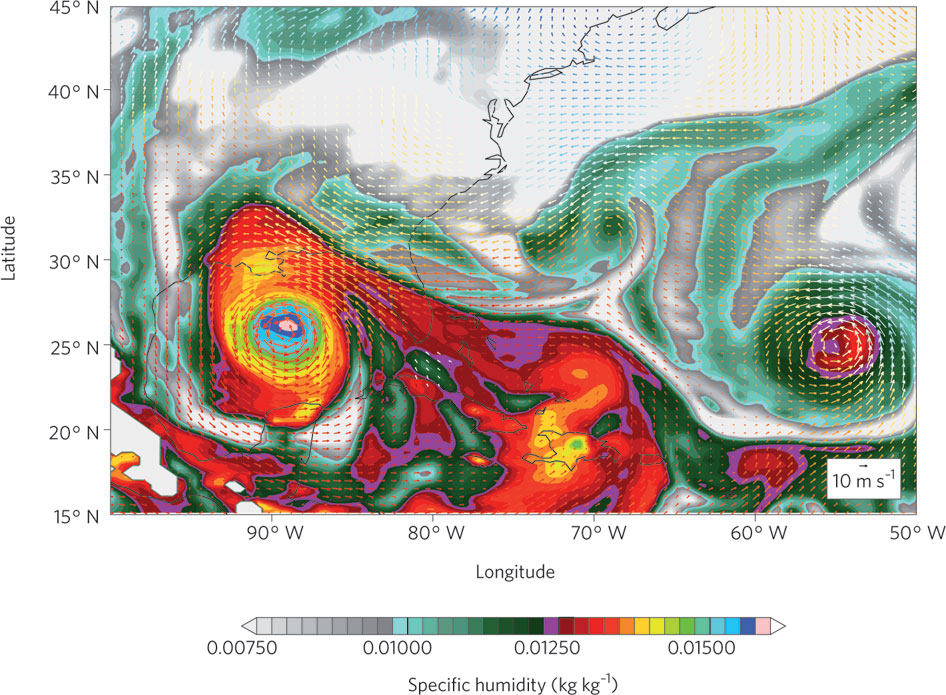
\includegraphics[width = 300pt]{MeteorologySimulation} 
		\caption{\textit{Symulacja dwóch tropikalnych huraganów nad Atlantykiem \cite{MeteorologySimulation}}}
\label{MeteorologySimulationImage}
\end{figure}

\begin{figure}[H]
	\centering
		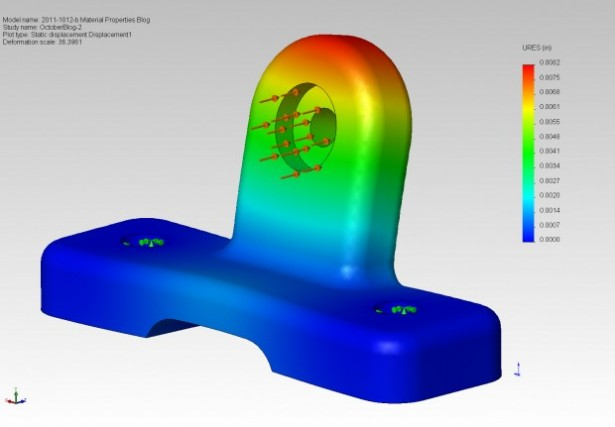
\includegraphics[width = 300pt]{EngineeringSimulation} 
		\caption{\textit{Analiza własności materiału za pomocą symulacji SolidWorks \cite{EngineeringSimulation}}}
\label{EngineeringSimulationImage}
\end{figure}

\newpage
Symulacje komputerowe można podzielić ze względu na:
\begin{itemize}
\item Charakter zdarzeń - deterministyczne, gdzie wyniki są powtarzalne i zależne tylko od zadanych parametrów i interakcji oraz stochastyczne - generowane losowo. 
\item Upływ czasu - ciągły, w którym chwile pośrednie są interpolowane brzegowymi lub dyskretny, gdzie czas zwiększa się przyrostowo.
\item Dane wyjściowe - statyczne, w których wynikiem jest konkretny zbiór danych lub dynamiczne, które ukazują cały proces trwający w czasie, np. animacja.
\end{itemize}

Przygotowywana praca realizuje symulator z deterministyczną przewidywalnością zdarzeń, czas zwiększa się stałymi przyrostami z możliwością ich modyfikowania. Przetwarzanie systemu odbywa się na pojedynczym komputerze, natomiast dane wyjściowe prezentowane są w postaci dynamicznej animacji.

\subsection{Układ dynamiczny}
\subsubsection{Wprowadzenie}
Układ dynamiczny jest to matematyczny model zjawiska występującego w przyrodzie, określany poprzez funkcję zachowania układu w danym czasie. Model ten jest zwykle opisany poprzez układ równań różniczkowych, zwanych równaniem stanu. W danej jednostce czasowej system posiada stan wyrażony jako wektor liczb utożsamiany z punktem w przestrzeni stanu. Ewolucja układu polega na wyznaczaniu kolejnych stanów na podstawie poprzednich poprzez użycie funkcji przejścia. Funkcja ta może być deterministyczna lub stochastyczna. W pierwszym przypadku dla zadanego czasu stan wyznaczany jest jednoznacznie, w drugim na ewolucję układu wpływają dodatkowe zdarzenia losowe. Przytoczone zagadnienie zostało szeroko omówione w \cite{MarciniakDynamicSystems}.

\subsubsection{Wahadło odwrócone na wózku}
\label{SubsectionPendulumIntro}
Niniejsza praca skupia się na modelu dynamiki układu złożonego z wahadła odwróconego umieszczonego na ruchomej platformie. Wahadło odwrócone to takie, w którym środek masy znajduje się powyżej punktu zaczepienia. Obiekt połączony jest z wózkiem, który porusza się w płaszczyźnie poziomej za pomocą silnika napędowego. Przykładowy układ pokazany został na ilustracji \ref{SystemModelImage}.

\begin{figure}[H]
	\centering
		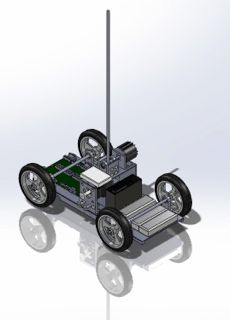
\includegraphics[width = 125pt]{SystemModel} 
		\caption{\textit{Model bezprzewodowego układu mechanicznego dla odwróconego wahadła na wózku \cite{SystemModel}}}
		\label{SystemModelImage}
\end{figure}

Przedstawione ustawienie wahadła powoduje, że znajduje się ono w niestabilnym punkcie równowagi. Punkt równowagi jest miejscem przy którym element pozostaje w bezruchu (prędkość zmiany stanu jest zerowa). Wahadło posiada dwa takie miejsca: stabilne znajdujące się poniżej punktu zaczepienia i niestabilnie powyżej tego punktu. W przypadku drugiego z nich nawet niewielkie zaburzenie stanu układu wywołuje ruch wahadłowy, który ustaje dopiero po zatrzymaniu się w stabilnym punkcie równowagi. 


Układ będący przedmiotem zainteresowania pokazany został na schemacie \ref{SytemSchemeImage}.

\begin{figure}[H]
	\centering
		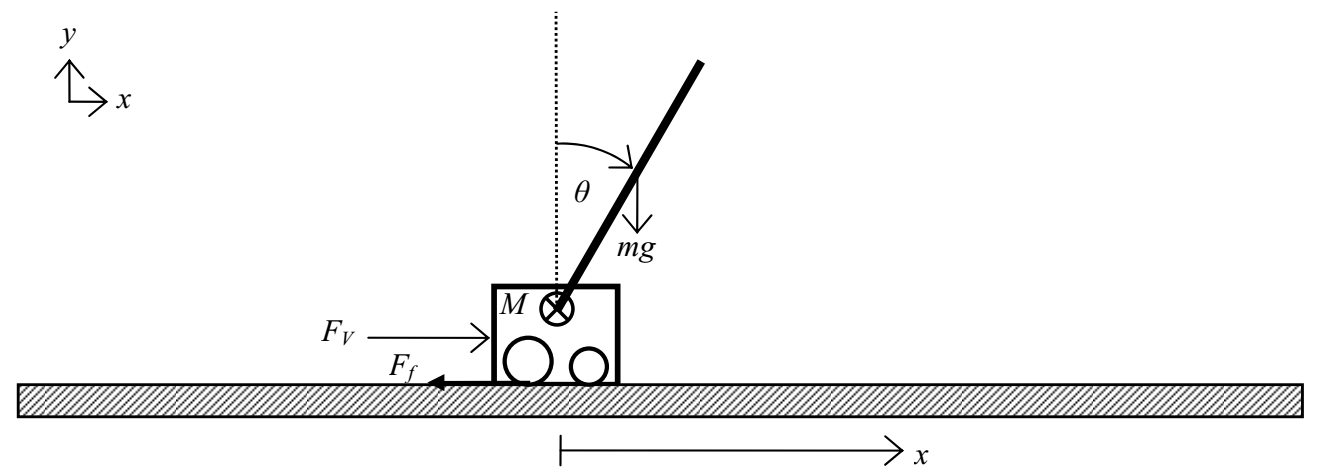
\includegraphics[width = 375pt]{SystemScheme} 
		\caption{\textit{Uproszczony schemat fizyki układu wahadła odwróconego na wózku \cite{LMIP} }}
		\label{SytemSchemeImage}
\end{figure}

Najważniejsze elementy fizyczne modelu:
\begin{itemize}
\item \(F_v\) - siła napędowa wózka \([N]\).
\item \(F_f\) - siła tarcia \([N]\).
\item \(m\) - masa wahadła \([kg]\). 
\item \(M\) - masa wózka \([kg]\).
\item \(g\) - przyspieszenie ziemskie \([\frac{m}{s^2}]\) 
\item \(\theta\) - kąt między osią wahadła a pionową osią układu \([rad]\).
\end{itemize}

Stan układu określany jest poprzez cztery parametry:
\begin{itemize}
\item Położenie środka wózka w osi O(X).
\item Prędkość liniowa wózka.
\item Kąt odchylenia wahadła od osi pionowej.
\item Prędkość kątowa wahadła.
\end{itemize}

Parametry fizyczne układu (wraz z nominalnymi wartościami opracowanymi w oparciu o \cite{LMIP}) pokazane zostały w tabeli \ref{table:NominalParameters}.
\begin{table}[H]
\begin{center}
\begin{tabular}{|c|c|}
  \hline 
  Parametr & Wartość\\
  \hline
  masa wózka & 0.79 \(kg\) \\
  \hline
  masa wahadła & 0.23 \(kg\) \\
  \hline
  długość wahadła & 0.61 \(m\) \\
  \hline
  współczynnik tarcia wózka & 7.68 \(\frac{N}{ms^{-1}}\) \\
  \hline
  współczynnik konwersji napięcia na siłę & 1.72 \(\frac{N}{V}\) \\
  \hline
\end{tabular} 
\end{center}
\caption{Parametry nominalne układu}
\label{table:NominalParameters}
\end{table}

Podstawowym zagadnieniem związanym z omawianym układem jest kontrola wychylenia wahadła. Urządzenie sterujące poprzez przyłożenie odpowiedniego napięcia na silniku wywołuje siłę napędową, która porusza platformą. Odpowiedni ruch podstawy pozwala na utrzymanie wahadła w punkcie równowagi.

\subsubsection{Trójwymiarowa wersja układu}
Dwuwymiarowy układ wahadła odwróconego na wózku można wykorzystać do zbudowania trójwymiarowego odpowiednika. Nowy model składa się z dwóch podukładów odpowiedzialnych za płaszczyzny związane z osiami głównymi układu, odpowiednio: O(XZ) i O(YZ). Przybliżony model znajduje się na rysunku \ref{3DimModel}.

\begin{figure}[H]
	\centering
		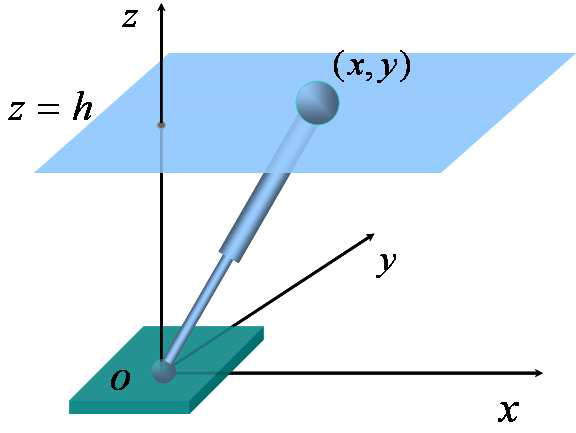
\includegraphics[width = 200pt]{3DimModel} 
		\caption{\textit{Uproszczony schemat trójwymiarowego układu wahadła odwróconego na wózku \cite{3DimModel}}}
		\label{3DimModel}
\end{figure}

Wynikowy stan całego układu określają stany poszczególnych komponentów. Ruch trójwymiarowego modelu wyznaczany jest jako złożenie (superpozycja) ruchów podukładów. Kierunek wychylenia wahadła można wyznaczyć za pomocą elementarnych własności geometrycznych. 

Opracowany w ten sposób model pozwala na poruszanie układem po płaszczyźnie O(XY). Wykorzystując odpowiednie narzędzie sterujące można dokonać stabilizacji układu nie tylko dla kąta odchylenia wahadła, ale również pozycji wózka na płaszczyźnie.

\section{Opis problemu}
\subsection{Motywacja}
Poruszone zagadnienie jest nietrywialną modyfikacją dobrze znanego zagadnienia sterowania wahadłem odwróconym na wózku. Wybrana tematyka pracy magisterskiej jest ściśle związana z zainteresowaniami autora pracy oraz materiałem realizowanym w ramach studiów. Przygotowanie pracy daje możliwość pogłębienia wiedzy z zakresu układów dynamiki i teorii sterowania. Dodatkowo pozwala na zmierzenie się z problemem wykonania symulacji, która w profesjonalny sposób zrealizuje postawione zadanie, a dodatkowo będzie atrakcyjna dla użytkownika końcowego. Ponadto wypracowana koncepcja systemu nie posiada jeszcze odzwierciedlenia we współczesnej technice. Toteż ze względu na elementy innowacyjności rozwiązania, pomysł ten jest okazją do analizy niestandardowego systemu, który może mieć zastosowanie w przyszłości, przynajmniej w środowisku wirtualnym.

\subsection{Główne cele}
Podstawowym celem pracy jest opracowanie symulatora transportera wahadła odwróconego na wózku. Zagadnienie to można w naturalny sposób podzielić na kilka podproblemów, co pozwala na szczegółowy przegląd poszczególnych elementów:
\begin{itemize}
\item Układ wahadła odwróconego na wózku. Projekt opiera się na analizie prostego modelu fizycznego wraz z implementacją jego zachowania. Dodatkowo rozszerza podstawową, dwuwymiarową wersję, na układ trójwymiarowy, by zwiększyć poziom skomplikowania, ocenić użyteczność zaproponowanego pomysłu i wzbogacić efekt końcowy. Kolejnym elementem jest wprowadzenie zakłóceń do układu w postaci podmuchów powietrza. Ważną rolę pełni również przegląd przypadków szczególnych i wypracowanie odpowiedniej reakcji na ich zaistnienie. Projekt powinien w pełni przedstawić zadane zagadnienie, umożliwić wprowadzanie modyfikacji układu i zapewnić pełny podgląd na stan układu. Dysponując w pełni zaimplementowanym modelem bazowym można przejść do badania zachowania układu wobec zadanych parametrów.
\item Stabilizacja układu. Naturalnym zagadnieniem wiążącym się z układem wahadła odwróconego na wózku jest próba stabilizacji wychylenia wahadła w obrębie pionowej osi układu. Komponent powinien pozostawać w niestabilnym punkcie równowagi. Celem projektu jest zrealizowanie wspomnianej stabilizacji za pomocą regulacji napięcia podawanego na wejście do silników sterujących wózkiem. Zadanie to wymaga wykorzystania wiedzy z zakresu teorii sterowania, w szczególności pojęcia regulatora. Praca powinna oprzeć się na implementacji odpowiednich narzędzi i przetestowaniu ich działania względem poszczególnych parametrów systemu. 
\item Transport układu. Osiągnięcie kontroli nad wychyleniem wahadła pozwala na dalsze rozszerzanie funkcjonalności systemu. Kolejnym etapem projektu jest stworzenie modułu sterującego ruchem całego układu. System powinien umożliwić stworzenie dowolnej trajektorii ruchu lub wczytanie przygotowanego przykładu, a następnie zmuszenie układu fizycznego do odwzorowania zadanej ścieżki ruchu.
\item Opracowanie symulatora. System nie będzie użyteczny, jeśli nie zostanie zaprezentowany użytkownikowi końcowemu w wygodnej i atrakcyjnej wizualnie formie. Ostatnim istotnym celem projektu jest stworzenie aplikacji okienkowej, której zadaniem będzie wizualizacja zachowania całego układu fizyki. Ponadto program powinien posiadać intuicyjny panel sterowania oraz dostarczać na bieżąco pełnej informacji na temat stanu sytemu. Dodatkowym walorem aplikacji może być tryb interaktywny, który pozwoli użytkownikowi nie tylko na przegląd mechaniki układu, lecz również na zabawę w sterowanie pojazdem.
\end{itemize}

\section{Przegląd istniejących rozwiązań}
\subsection{Symulatory}
W obecnych czasach oprogramowanie symulacyjne jest podstawą funkcjonowania wielu gałęzi przemysłu. Przed przystąpieniem do realizacji projektu autor pracy skupił się na przeglądzie najbardziej popularnych narzędzi symulacyjnych w celu znalezienia kluczowych cech, jakie powinien spełniać dobry symulator. Na szczególną uwagę zasługują trzy rozwiązania:
\begin{itemize}
\item Simulink - pakiet numeryczny MATLAB firmy The MathWorks służący do przeprowadzania symulacji komputerowych. Narzędzie pozwala na tworzenie modeli poprzez wybór komponentów z interfejsu graficznego. Zapewnia symulację z czasem dyskretnym i ciągłym. Simulink wykorzystywany jest głównie do cyfrowego przetwarzania sygnałów, teorii sterowania i analizy obwodów elektrycznych.
\item LabVIEW - środowisko programistyczne firmy National Instruments skupiające się głównie na pomiarach i analizie danych. Pozwala na tworzenie modeli poprzez specjalny graficzny język programowania. LabVIEW znajduje zastosowanie w ośrodkach badawczych i testach przemysłowych.
\item SolidWorks Simulation - pakiet symulacyjny będący częścią programu komputerowego typu CAD firmy Dassault Systèmes. Umożliwia analizę modeli pod wieloma kątami technicznym oraz symulację ruchu układu w obecności różnych czynników zewnętrznych. Narzędzie wykorzystywane jest przez wiodące firmy z wielu gałęzi przemysłu.  
\end{itemize}

Przytoczone przykłady zostały przeanalizowane pod kątem budowy, możliwości technicznych, sposobu prezentacji danych i interakcji z użytkownikiem. Wypracowane wnioski dały gruntowną podstawę do stworzenia własnego rozwiązania opartego na kilku najważniejszych cechach:
\begin{itemize}
\item Modularna budowa - program powinien być zbudowany z respektowaniem standardów inżynierii oprogramowania. Poszczególne funkcjonalności powinny być wyodrębnione i tworzyć pojedyncze pakiety, które będzie można wykorzystywać jako samodzielne elementy.
\item Prostota - konkretne narzędzie powinno spełniać wszystkie wymagania techniczne i ukazywać rezultaty w jak najbardziej przejrzysty sposób. Dodatkowe elementy powodują jedynie przesłonięcie kluczowych funkcjonalności.
\item Dostęp do danych - symulacja powinna w każdej chwili udostępniać komplet niezbędnych danych fizycznych, wizualizować stan zadanego układu oraz gromadzić istotne parametry w formie wykresów lub diagramów.
\item Sterowanie - modyfikacja parametrów symulacji powinna być intuicyjna dla każdego użytkownika.
\end{itemize}
\subsection{Dynamika i sterowanie}
Zagadnienie stabilizacji dwuwymiarowego układu wahadła odwróconego na wózku zostało szeroko omówione w wielu pracach naukowych. Ze względu na prostotę podstawowego modelu temat ten często pojawia się jako materiał na laboratorium na studiach poświęconych automatyce i robotyce (przykładem jest instrukcja \cite{LMIP}).

Dokładna analiza problemu opiera się na wyborze jednego z modeli: nieliniowego lub uproszczonego, po linearyzacji. W pierwszym przypadku model wiernie odwzorowuje zachowanie wahadła niezależnie od jego wychylenia, w drugim pojawia się ograniczenie na nieznaczne wychylenia wahadła. Większość przeanalizowanych prac realizuje drugie założenie ze względu na znaczne uproszczenia obliczeń przy niewielkiej utracie dokładności. Kolejnym wyróżnikiem jest sposób stabilizacji układu. Istnieje wiele narzędzi z zakresu teorii sterowania, które pozwalają na kontrolowanie układu. Najbardziej popularnymi są regulatory: PID i LQR. Szczegółowy przegląd i porównanie narzędzi zostało omówione w artykule \cite{OptimalControl}. Autor pracy skupił się wyłącznie na sterowaniu regulatorem PID, jednakże pozostawił możliwość zamiany kontrolera na dowolny inny.

Zagadnienie trójwymiarowego układu znajduje odniesienie w modelowaniu ruchu dwunożnego robota, w którym skomplikowany model zostaje zastąpiony odpowiednimi wahadłami odwróconymi. Stabilizacja uproszczonego modelu pozwala na poruszanie robotem przy zachowaniu stabilności jego postawy. Temat został gruntownie przedstawiony w artykule \cite{BipedWalking}.

Symulacja transportu układu nie jest zagadnieniem szeroko omówionym, toteż autor pracy oparł rozwiązanie na ogólnej wiedzy z zakresu dynamiki układów i sterowania. 


%% -------- chapter II --------
\newpage
\chapter{Definicja projektu}
\section{Zakres projektu}
Projekt obejmuje opracowanie biblioteki fizyki dla transportera wahadła odwróconego na wózku oraz symulatora wizualizującego działanie biblioteki. Aplikacja przeznaczona jest na platformę Windows. Projekt podzielony jest na kilka głównych elementów:
\begin{itemize}
\item Budowa dynamiki układu w oparciu o podstawy matematyczno-fizyczne.
\item Opracowanie modułu kontroli układem w celu zapewnienia stabilności.
\item Wprowadzenie modułu zakłóceń w postaci siły wiatru.
\item Obsługa trajektorii ruchu.
\item Wizualizacja układu na trójwymiarowej scenie.
\item Zarządzanie animacją i modyfikacja parametrów układu.
\item Umożliwienie użytkownikowi ręcznej kontroli systemu poprzez tryb gry.
\end{itemize}

\section{Analiza wymagań}
Wymagania względem projektu można podzielić na funkcjonalne i niefunkcjonalne. Pierwsze odnoszą się do konkretnych zadań, jakie aplikacja powinna realizować. Drugie dotyczą ogólnych cech jakimi program powinien się charakteryzować.

Podstawowe wymagania niefunkcjonalne:
\begin{itemize}
\item Użyteczność - program powinien w pełni realizować postawione zadania, a dodatkowo zachęcać użytkownika do zapoznania się z tematyką.
\item Stabilność - aplikacja powinna działać poprawnie bez względu na interakcję użytkownika.
\item Łatwość użytkowania - korzystanie z funkcjonalności powinno być intuicyjne, ponadto wszystkie najważniejsze informacje powinny zostać zebrane w charakterze pomocy.
\item Łatwość modyfikowania - program powinien umożliwiać dostosowywanie ustawień w zależności od potrzeb użytkownika. 
\item Modularność - każdy element systemu powinien być skonstruowany jako oddzielny moduł udostępniający szereg funkcji.
\item Rozszerzalność - kod źródłowy aplikacji powinien być przejrzysty i łatwy do zarządzania.
\end{itemize}

Najważniejsze wymagania funkcjonalne:
\begin{itemize}
\item Zarządzanie aplikacją
\begin{itemize}
\item Wybór jednego z trybów działania aplikacji (stabilizacja układu, śledzenie trajektorii, tryb gry).
\item Modyfikacja parametrów startowych układu.
\item Możliwość ustawienia aktualnego regulatora i generatora wiatru.
\item Modyfikacja dokładności śledzenia trajektorii.
\item Zarządzanie parametrami wiatru w trakcie przebiegu animacji.
\item Wybór trajektorii z zestawu przygotowanych przykładów.
\item Możliwość stworzenia nowej trajektorii poprzez zadanie jej parametryzacji.
\end{itemize}
\item Wizualizacja
\begin{itemize}
\item Trójwymiarowa scena z możliwością swobodnej manipulacji kamerą.
\item Umieszczenie modelu transportera w postaci platformy na kołach z przyczepionym odwróconym wahadłem.
\item Wyświetlanie płaszczyzny, po której porusza się model, wraz z podziałką metryczną. 
\item W zależności od ustawień wyświetlania, pokazywanie trajektorii ruchu wahadła i wózka.
\item Kontrolowanie postępu animacji poprzez odpowiedni panel.
\item Możliwość przełączania wyświetlania między trybami graficznymi.
\item Możliwość ręcznego sterowania układem za pomocą myszy i klawiatury.
\end{itemize}
\item Prezentacja danych
\begin{itemize}
\item Dynamiczne wykresy dla kluczowych danych, tj. uchyb regulacji czy podawane napięcie na silniku.
\item Możliwość zapisywania wygenerowanych wykresów.
\item Wyświetlanie aktualnego stanu układu.
\item Prezentacja informacji ogólnych na temat aplikacji i dynamiki układu
\item Okno pomocy opisujące podstawowe funkcjonalności programu.
\end{itemize}
\end{itemize}

\section{Ograniczenia}
W trakcie wstępnej analizy projektu przyjęto zestaw ograniczeń w celu zachowania spójności pracy i uniknięcia nadmiernego rozszerzania mniej istotnych elementów. Są to:
\begin{itemize}
\item Konieczność spełnienia wszystkich podstawowych wymagań wymienionych w poprzedniej sekcji.
\item Możliwość uproszczenia modelu w celu zmniejszenia złożoności obliczeń.
\item Ograniczenie realizacji stabilizacji układu do wykorzystania kilku odmian regulatora PID.
\item Ograniczenie jakości wizualizacji do wyświetlania prostego modelu układu na trójwymiarowej scenie.
\end{itemize}

%% -------- chapter III --------
\newpage
\chapter{Opis rozwiązania}
\section{Podstawy matematyczno-fizyczne}
Dokładne omówienie rozwiązań przyjętych w pracy wymaga rozwinięcia kilku zasadniczych pojęć. Przytoczone zagadnienia zostały opracowane w oparciu o materiały z wykładów poświęconych projektowaniu środowiska wirtualnego: \cite{MarciniakControlSystems} oraz \cite{MarciniakClosedLoop}, a także pozycję \cite{RungeKutta}.

\subsection{Równania stanu}
\label{StateSpaceSubsection}
Stan układu jest to informacja umożliwiająca określenie zachowania układu w danej jednostce czasu. Zawiera w sobie zakumulowane dane z całego przebiegu ruchu od chwili początkowej do obecnej. Jest to tzw. własność pamięci układu. Istotnym zagadnieniem związanym ze stanem układu jest charakterystyka związków między jego zmiennymi. Związki te określane są mianem równania stanu. Równanie to przyjmuje postać równania różniczkowego pierwszego rzędu i stanowi matematyczny model układu fizycznego.

Pojedynczy stan można określić jako wektor zmiennych będący punktem w n-wymiarowej przestrzeni stanów. Wówczas dynamikę układu można przedstawić poprzez n-wymiarową rozmaitość różniczkową \(N\) z powiązanym prostopadłym polem wektorowym \(\mathbf{v}(\mathbf{x},t)\). Trajektorie elementów układu dynamicznego wyrazić można poprzez równanie:
\begin{equation} \label{eq_1}
\dot{\mathbf{x}} = \mathbf{v}(\mathbf{x},t)
\end{equation}
z zadanym warunkiem początkowym:
\begin{equation}
\mathbf{x}(t_0) = \mathbf{x_0}
\end{equation}
W sytuacji gdy prawa strona równania \ref{eq_1} nie zależy od czasu przyjmuje się, że układ dynamiczny jest autonomiczny. Wówczas wyznaczenie punków stacjonarnych układu polega na rozwiązaniu równania:
\begin{equation}
\mathbf{0} = \mathbf{v}(\mathbf{x})
\end{equation}

Przedstawiony model jest jednoznacznie zdefiniowany przez warunek początkowy. Jednakże w rozwiązaniach praktycznych dużo korzystniejszym podejściem jest stworzenie rozwiązania, które oprócz obserwacji umożliwia również kontrolę. Aby to osiągnąć uzupełnia się model o dodatkowy wektor \(\mathbf{u}\) zawierający parametry modyfikujące trajektorie układu. Odpowiednie równanie trajektorii przybiera wówczas następującą postać:
\begin{equation}
\dot{\mathbf{x}} = \mathbf{v}(\mathbf{x},\mathbf{u})
\end{equation}

W większości przypadków aplikacje symulacyjne nie wymagają rozwiązywania skomplikowanego nieliniowego równania. Toteż często stosowaną praktyką jest upraszczanie poprzez linearyzację układu. W przypadku układu autonomicznego zmienność zostaje zastąpiona stałymi elementami: macierzą \(A\) związaną ze stanem układu oraz macierzą \(B\) związaną ze sterowaniem. Dodatkowo należy przyjąć, że w niektórych systemach zmienne stanu mogą być niedostępne w sposób bezpośredni, dlatego należy zdefiniować dodatkowe równanie pozwalające wyprowadzić zmienne wyjściowe układu.

Ostatecznie równania stanu dla systemu liniowego niezmienniczego w czasie (ang. Linear Time Invariant) wygląda w sposób następujący:
\begin{gather}
\dot{x}(t) = Ax(t) + Bu(t) \\
y(t) = Cx(t) + Du(t)
\end{gather}
gdzie:
\begin{itemize}
\item \(x(t)\) - wektor stanu,
\item \(u(t)\) - wektor sterowania,
\item \(u(t)\) - wektor wyjściowy,
\item \(A^{q \times n}\) - macierz stanu,
\item \(B^{q \times m}\) - macierz sterowania,
\item \(C^{p \times n}\) - macierz wyjścia,
\item \(D^{p \times m}\) - macierz sterowania bezpośredniego.
\end{itemize}

Parametry \(q\) i \(p\) są zwykle równe \(n\), toteż macierz stanu jest najczęściej macierzą kwadratową. Macierz \(D\) pojawia się tylko w przypadku układów właściwych, czyli takich które posiadają transmitancję właściwą.

Model równań stanu dla układu ciągłego ilustruje schemat \ref{StateSpace}.

\begin{figure}[H]
	\centering
		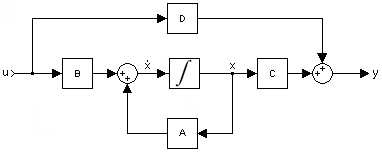
\includegraphics[width = 300pt]{StateSpace} 
		\caption{\textit{Schemat równań stanu dla układu ciągłego \cite{StateSpace}}}
		\label{StateSpace}
\end{figure}

\subsection{Algorytm Rungego-Kutty}
\label{Runge}
Algorytm Rungego-Kutty jest to iteracyjna metoda rozwiązywania równań i układów równań różniczkowych zwyczajnych. Określenie to stosuje się również do całej rodziny jawnych i niejawnych metod z uwzględnieniem pewnych modyfikacji. Zwyczajowo jednak przyjmuje się konkretną implementację w postaci metody czwartego rzędu. 

Zadaniem algorytmu jest wyznaczenie rozwiązania \(y\) na podstawie równania postaci \(\dot{y} = f(x,y)\) oraz wartości początkowej  \(y(x_0) = y_0\). Ustalając krok całkowania \(h\) można wyznaczyć rozwiązanie w sposób iteracyjny:
\begin{equation*}
\begin{aligned}
y_{n+1} &= y_{n} + \Delta y_n \\
\Delta y_n &= \frac{1}{6}(k_1 + 2k_2 +2k_3 +k_4)
\end{aligned}
\end{equation*}
Współczynniki \(k_{1...4}\) wyznaczane są następująco:
\begin{equation*}
\begin{aligned}
k_1 &= hf(x_n, y_n) \\
k_2 &= hf(x_n + \frac{h}{2}, y_n + \frac{k_1}{2}) \\
k_3 &= hf(x_n + \frac{h}{2}, y_n + \frac{k_2}{2}) \\
k_4 &= hf(x_n + h, y_n + k_3)
\end{aligned}
\end{equation*}

Rezultatem działania metody jest zestaw kolejnych punków przybliżających rozwiązanie. W przypadku układu równań różniczkowych postępowanie jest analogiczne. 

Rozwiązanie opracowane przez autora pracy korzysta z modyfikacji bazowego algorytmu zwanej metodą Casha-Karpa, która pozwala na adaptacyjny dobór parametru kroku całkowania \(h\).

\subsection{SLERP}
\label{SLERP}
SLERP (ang. spherical linear interpolation) jest to interpolacja wprowadzona przez Kena Shoemake w celach animacji rotacji trójwymiarowych. Technika zapewnia gładki ruch ze stałą prędkością między punktami końcowymi.

SLERP bazuje na fakcie, że każdy punkt krzywej, po której porusza się obiekt jest kombinacją liniową punktów końcowych animacji: $p_0$ i $p_1$. Niech t będzie parametrem takim, że: $0 \leqslant t \leqslant 1$. Dodatkowo niech $\omega$ będzie kątem zakreślanym w trakcie przejścia, więc spełniającym równanie $cos(\omega) = p_0 \cdot p_1$.
Wówczas formuła geometryczna interpolacji wygląda następująco:
\begin{equation*}
SLERP(p_0, p_1, t) = \frac{sin((1-t)\omega)}{sin(\omega)} p_0 + \frac{sin(t\omega)}{sin(\omega)} p_1
\end{equation*}

\subsection{Regulator PID}
\label{PIDSection}
Regulator PID (ang. proportional-integral-derivative controller) jest to element obwodu regulacji, którego głównym zadaniem jest generowanie odpowiedniego sygnału sterującego, zmuszającego układ do określonego zachowania. Narzędzie to jest bardzo często wykorzystywane w przemysłowych układach regulujących. Regulator ustawiony jest w pętli sprzężenia zwrotnego. W trakcie jednego cyklu wyznacza różnicę między wartością docelową i obecną (uchyb) oraz podaje na wejście regulowanego układu sygnał kompensujący uchyb.


 Regulator PID składa się z trzech komponentów:
\begin{itemize}
\item człon proporcjonalny \textbf{P}, który reaguje na obecne wartości uchybu,
\item człon całkujący \textbf{I}, który przechowuje informację na temat poprzednich wartości uchybu,
\item człon różniczkujący \textbf{D}, który przewiduje następne wartości uchybu.
\end{itemize}

Schemat poglądowy regulatora PID zawarty został na ilustracji \ref{PID}.

\begin{figure}[H]
	\centering
		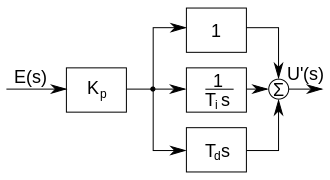
\includegraphics[width = 250pt]{PID} 
		\caption{\textit{Schemat blokowy idelnego regulatora PID \cite{PID}}}
		\label{PID}
\end{figure}

Sygnał wyjściowy z regulatora jest sumą ważoną poszczególnych komponentów. Regulator wykonuje algorytm:
\begin{equation} \label{PIDAlg}
u(t) = K_p[e(t) + \frac{1}{T_i}\int_{0}^{t} e(\tau) d\tau + T_d \frac{de(t)}{dt}]
\end{equation}
gdzie:
\begin{itemize}
\item $u(t)$ - sygnał sterujący z regulatora,
\item $e(t)$ - uchyb regulacji,
\item $K_p$ - wzmocnienie członu proporcjonalnego,
\item $T_i$ - czas zdwojenia członu całkującego,
\item $T_d$ - czas wyprzedzenia członu różniczkującego.
\end{itemize}

Algorytm \ref{PIDAlg} można poddać dyskretyzacji z krokiem całkowania $h$. Poszczególne iteracje będą wówczas wyznaczane w następujący sposób:
\begin{equation}
u(i) = K_p[e(i) + \frac{h}{T_i} \sum_{k=0}^{i} e(k) + T_d \frac{e(i) - e(i-1)}{h}]
\end{equation}

Uzyskanie poprawnego działania regulatora PID wymaga dobrania odpowiednich wartości nastaw. Optymalizacji parametrów dokonuje się poprzez ręczne strojenie lub wyznaczenie algorytmiczne (np. metodą Zieglera-Nicholsa). Warto przy okazji zwrócić uwagę na to, że regulator PID nie gwarantuje optymalnego sterowania ani stabilności układu. W celu uzyskania powyższych cech należy rozważyć zastosowanie innego typu regulacji np. regulatora LQR.

\subsection{Regulator podwójny PID}
\label{DoublePID}
Utrzymanie układu wahadła odwróconego na wózku w niestabilnym punkcie równowagi wymaga uzupełnienia systemu o mechanizm kontroli. Regulator PID może pełnić funkcję narzędzia utrzymującego zerowe odchylenie wahadła względem osi pionowej. Niestety, w sytuacji, gdy celem układu jest dodatkowo stabilizacja położenia, nie wystarczy pojedynczy regulator PID. Rozwiązaniem tego problemu jest rozbudowa struktury na dwa komponenty odpowiedzialne za poszczególne wielkości regulowane. W literaturze pojawia się kilka zagadnień, z których najbardziej popularne to:
\begin{itemize}
\item Układ regulacji kaskadowej pokazany na rysunku \ref{DoublePIDCascade}. Jest to klasyczne podejście zbudowane na podstawie ''szybkiej'' pętli wewnętrznej i ''wolnej'' pętli zewnętrznej. Regulator nadrzędny odpowiada za sterowanie położeniem wózka. Wartość wyjściowa z regulatora staje się wartością zadaną dla wewnętrznego układu, który zajmuje się regulacją kąta odchylenia wahadła od pionu. Wyjście z regulatora wewnętrznego podawane jest ostatecznie do sterowanego układu. Koncepcja ta pozwala na utrzymanie stabilności wahadła z dodatkowym uwzględnieniem dostosowywania pozycji wózka.

\begin{figure}[H]
	\centering
		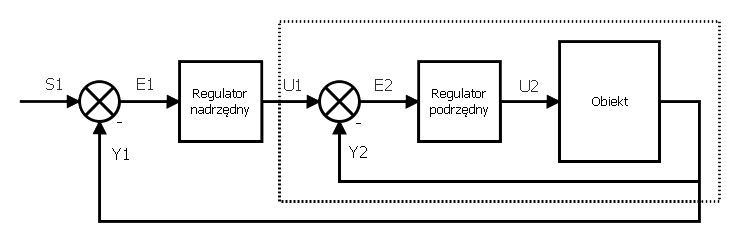
\includegraphics[width = 350pt]{DoublePIDCascade} 
		\caption{\textit{Schemat blokowy kaskadowego układu sterowania regulatorami PID\cite{JTJT}}}
		\label{DoublePIDCascade}
\end{figure}

\item Układ regulacji równoległej pokazany na ilustracji \ref{DoublePIDParallel}. Działanie tego układu jest zbliżone do wariantu kaskadowego. Cechą odrębną jest fakt, że sterowanie podawane na układ wyznaczane jest jako różnica sterowań poszczególnych podukładów sterujących. Rozwiązanie to generuje problem wzajemnego zakłócania regulatorów, toteż należy uwzględnić w modelu, że regulator odchylenia wahadła musi być ''szybszy'' od regulatora położenia. Zabieg ten spowoduje, że tylko sterownik położenia potraktuje dodatkowe sterowanie jako zakłócenie.

\begin{figure}[H]
	\centering
		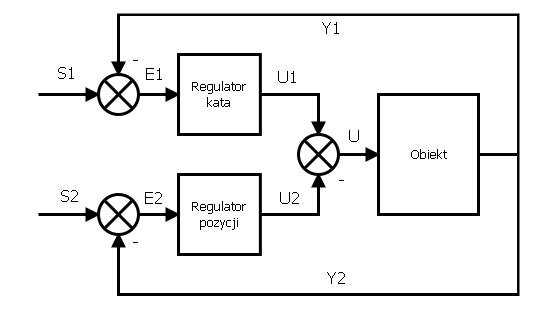
\includegraphics[width = 300pt]{DoublePIDParallel} 
		\caption{\textit{Schemat blokowy równoległego układu sterowania regulatorami PID\cite{JTJT}}}
		\label{DoublePIDParallel}
\end{figure}
\end{itemize}

Definicja oznaczeń na schematach \ref{DoublePIDCascade} i \ref{DoublePIDParallel}:
\begin{itemize}
\item S1, S2 - wartości zadanie,
\item E1, E2 - uchyby regulacji,
\item U1, U2 - wyjścia z regulatorów,
\item Y1, Y2 - wyjścia z układu sterowanego.
\end{itemize}  

\section{Mechanika systemu}
\subsection{Model matematyczny ruchu}
\label{MathModel}
\subsubsection{Schemat}
Wykonanie poprawnej symulacji dowolnego zjawiska fizycznego wymaga na wstępie stworzenia odpowiedniego modelu matematycznego, który przybliży charakterystykę danego zjawiska. Niniejsza sekcja poświęcona jest omówieniu modelu ruchu wahadła odwróconego na wózku. Pełny model zrealizowany w projekcie zawiera w sobie dwa wspomniane układy, które są ze sobą połączone. Jednakże ich niezależność pozwala na swobodne rozpatrywanie pojedynczego układu. Wstępne informacje na temat zadania zostały przedstawione w sekcji \ref{SubsectionPendulumIntro}. Dalsze rozważania będą dotyczyły analizy rozkładu sił w modelu oraz wyprowadzenia równań ruchu na podstawie pracy \cite{LMIP}.

W przyjętym rozwiązaniu skupiono się na podstawowych siłach rządzących światem rzeczywistym. Ruch układu odbywa się w obecności siły grawitacji o przyspieszeniu ziemskim $g$. Na wózek działają dodatkowo siły: tarcia $F_f$ i napędu pochodzącego od silnika $F_v$. Nacisk wózka $Mg$ równoważony jest przez siłę sprężystości podłoża $N$. Ponadto należy rozważyć siły wzajemnego oddziaływania między wózkiem a wahadłem: $F_x$ i $F_y$ bazując na trzeciej zasadzie dynamiki Newtona:
\begin{quote}
W inercjalnym układzie odniesienia siły wzajemnego oddziaływania dwóch ciał mają takie same wartości, taki sam kierunek, przeciwne zwroty i różne punkty przyłożenia.
\end{quote}

Pełny rozkład sił, wraz z zaznaczeniem użytecznych odległości, przedstawiony został na schemacie \ref{SystemForces}.

\begin{figure}[H]
	\centering
		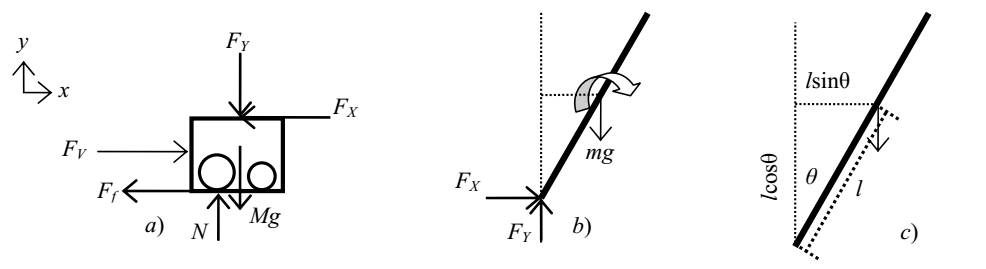
\includegraphics[width = 400pt]{SystemForces} 
		\caption{\textit{Schemat rozkładu sił dla: a) wózka, b) wahadła, c) odległości między komponentami \cite{LMIP}}}
		\label{SystemForces}
\end{figure}

Idealny model wahadła zakłada, że składa się ono z obiektu masowego zawieszonego na nierozciągliwej cienkiej nici o długości $l$. Wobec tego można przyjąć, że ogół sił pochodzących od wahadła skupiony jest w obrębie jego środka masy. Uwzględniając fakt, że punkt zaczepienia wahadła znajduje się na środku wózka, którego pozycja określona jest współrzędną $x$, lokację środka masy można wyznaczyć jako:
\begin{equation} \label{MassCenter}
\begin{aligned}
x_g &= x + lsin(\theta)\\
y_g &= lcos(\theta)
\end{aligned}
\end{equation}

Siła napędowa pochodząca od silnika powoduje, że układ zyskuje zdolność do wymuszonego poruszania się po powierzchni. Siła ta regulowana jest poprzez napięcie przyłożone do silnika. Wzór na wyznaczenie tej siły wygląda następująco:
\begin{equation} \label{Voltage}
F_v = \gamma_v V
\end{equation}
gdzie $\gamma_f$ jest stałym współczynnikiem konwersji napięcia na siłę.

\newpage
Siła tarcia związana jest z oddziaływaniem między wózkiem a podłożem. W analizowanym modelu wykorzystano zjawisko tarcia kinetycznego zależnego od prędkości ruchu, które można wyznaczyć jako:
\begin{equation} \label{Friction}
F_f = \gamma_f \frac{dx}{dt}
\end{equation}
gdzie $\gamma_f$ jest stałym współczynnikiem tarcia wózka.

\subsubsection{Ruch postępowy}
Analiza ruchu postępowego została podzielona na dwa podproblemy związane z osiami głównymi układu oraz rozpatrzona oddzielnie dla wózka i wahadła. Umożliwia to przejrzyste zbadanie oddziaływań i łatwe wyprowadzenie równań ruchu. W przypadku wahadła można określić ruch w pionie i w poziomie, dla wózka tylko poziomy. 

Zachowanie układu zostało scharakteryzowane w oparciu o drugie prawo dynamiki Newtona, które mówi:
\begin{quote}
W układzie inercjalnym, suma sił $F$ działających na ciało jest równa masie ciała $m$ pomnożonej przez jego przyspieszenie $a$:
\end{quote}
\begin{equation} \label{Newton}
F = ma
\end{equation}

Korzystając z przytoczonego twierdzenia \ref{Newton} zależność dla wózka w poziomie wygląda następująco:
\begin{equation}
F_v - F_x - F_f = M \frac{d^2x}{dt^2}
\end{equation}

Po uwzględnieniu charakterystyki siły napędu silnika \ref{Voltage} i siły tarcia \ref{Friction}:
\begin{equation} \label{CartX}
\gamma_v V - F_x - \gamma_f \frac{dx}{dt} = M \frac{d^2x}{dt^2}
\end{equation}

Analogicznie dla wahadła ruch w poziomie można określić równaniem:
\begin{equation} \label{PendulumX}
F_x = m \frac{d^2x_g}{dt^2}
\end{equation}

Dalsze rozważania wymagają wyznaczenia pierwszej i drugiej pochodnej czasowej po poziomej trajektorii środka masy wahadła.

Dla pierwszej pochodnej należy skorzystać z \ref{MassCenter}:
\begin{equation} \label{FirstDerivative}
\frac{dx_g}{dt} = \frac{d(x + lsin(\theta))}{dt} = \frac{dx}{dt} + lcos(\theta)\frac{d\theta}{dt}
\end{equation}

Wyznaczenie drugiej pochodnej można uzyskać poprzez różniczkowanie równania \ref{FirstDerivative}:
\begin{equation} \label{Second}
\begin{aligned}
\frac{d^2x_g}{dt^2} &= \frac{d}{dt}(\frac{dx}{dt} + lcos(\theta)\frac{d\theta}{dt})\\
&= \frac{d^2x}{dt^2} + l(\frac{dcos(\theta)}{dt} \frac{d\theta}{dt} + cos(\theta) \frac{d^2\theta}{dt^2})\\
&= \frac{d^2x}{dt^2} - lsin(\theta)(\frac{d\theta}{dt})^2 + lcos(\theta) \frac{d^2\theta}{dt^2}
\end{aligned}
\end{equation}

Wykorzystując wyznaczone pochodne oraz równanie \ref{PendulumX} można wyznaczyć poziomą siłę reakcji miedzy wózkiem a wahadłem:
\begin{equation} \label{ReactionX}
F_x = m (\frac{d^2x}{dt^2} - lsin(\theta)(\frac{d\theta}{dt})^2 + lcos(\theta) \frac{d^2\theta}{dt^2})
\end{equation}

Po wstawieniu uzyskanych wyprowadzeń do równania ruchu wózka w poziomie \ref{CartX} i dokonaniu uporządkowania zmiennych ostateczna postać równania wygląda następująco:
\begin{equation} \label{CartFullX}
(M + m) \frac{d^2}{dt^2} + \gamma_f \frac{dx}{dt} = \gamma_v V + mlsin(\theta)(\frac{d\theta}{dt})^2 - mlcos(\theta) \frac{d^2\theta}{dt^2}
\end{equation}

W przypadku ruchu w pionie należy rozważyć wyłącznie ruch wahadła. Bazując na twierdzeniu \ref{Newton} równanie ruchu można podać w postaci:
\begin{equation} \label{PendulumY}
F_y - mg = m \frac{d^2y_g}{dt^2}
\end{equation}

Podobnie jak dla ruchu w poziomie niezbędne będzie wyznaczenie pochodnych czasowych trajektorii środka masy.

Pierwsza pochodna przybiera postać:
\begin{equation}
\frac{dy_g}{dt} = \frac{d(lcos(\theta))}{dt} = -lsin(\theta) \frac{d\theta}{dt}
\end{equation}

Druga pochodna:
\begin{equation}
\begin{aligned}
\frac{d^2y_g}{dt^2} &= \frac{d}{dt}(-lsin(\theta) \frac{d\theta}{dt})\\
&= -l(\frac{dsin(\theta)}{dt}\frac{d\theta}{dt} + sin(\theta) \frac{d^2\theta}{dt^2})\\
&= -lcos(\theta)(\frac{d\theta}{dt})^2 - lsin(\theta) \frac{d^2\theta}{dt^2}
\end{aligned}
\end{equation}

\newpage
Łącząc wyznaczone pochodne z równaniem \ref{PendulumY} można wyprowadzić wzór na pionową siłę reakcji między wózkiem a wahadłem:
\begin{equation} \label{ReactionY}
F_y = mg - mlcos(\theta) (\frac{d\theta}{dt})^2 - mlsin(\theta) \frac{d^2\theta}{dt^2}
\end{equation}

Wzór ten będzie niezbędny do dalszych rozważań poświęconych ruchowi obrotowemu.

\subsubsection{Ruch obrotowy}
Ruch obrotowy układu przejawia się w dynamice wahadła, które obraca się względem zadanego punktu zaczepienia.
Analiza tego ruchu została przeprowadzona w oparciu o drugą zasadę dynamiki ruchu obrotowego:
\begin{quote}
Jeśli na ciało, o momencie bezwładności względem osi obrotu $I$, działają zewnętrzne siły o wypadkowym momencie siły $M$, to w rezultacie tego oddziaływania ciało będzie obracać się z przyspieszeniem kątowym $\epsilon$ takim, że:
\end{quote}
\begin{equation}
M = I \epsilon
\end{equation}
Moment siły i przyspieszenie kątowe są pseudowektorami o zgodnych kierunkach i zwrotach. Poszczególne siły $\mathbf{F}$ o wektorach pozycji $\mathbf{r}$ generują momenty sił  zdefiniowane jako:
\begin{equation}
\overline{M} = \mathbf{F} \times \mathbf{r}
\end{equation}

Sumując wszystkie momenty sił działające na środek masy wahadła można uzyskać wzór:
\begin{equation}
F_y l sin(\theta) - F_x lcos(\theta) = I\frac{d^2\theta}{dt^2}
\end{equation}

Korzystając z wyznaczonych wcześniej sił reakcji \ref{ReactionX} i \ref{ReactionY} wzór przyjmie postać:
\begin{equation}
\begin{aligned}
&(mg + -mlcos(\theta) (\frac{d\theta}{dt})^2 - mlsin(\theta) \frac{d^2\theta}{dt^2})lsin(\theta)\\
&-m (\frac{d^2x}{dt^2} - lsin(\theta)(\frac{d\theta}{dt})^2 + lcos(\theta) \frac{d^2\theta}{dt^2})lcos(\theta) = I\frac{d^2\theta}{dt^2}
\end{aligned}
\end{equation}

Po wymnożeniu i pogrupowaniu poszczególnych elementów wzór wygląda następująco:
\begin{equation}
mglsin(\theta) - ml^2(sin^2(\theta) + cos^2(\theta) \frac{d^2\theta}{dt^2} - mlcos(\theta) \frac{d^2x}{dt^2} = I\frac{d^2\theta}{dt^2}
\end{equation}

Korzystając z trywialnej równości trygonometrycznej
\begin{equation}
sin^2(\theta) + cos^2(\theta) = 1
\end{equation}

oraz dokonując kolejnego pogrupowania, ostateczną postać równania ruchu obrotowego wahadła można wyrazić jako:
\begin{equation}
(I + ml^2)\frac{d^2\theta}{dt^2} = mglsin(\theta) - mlcos(\theta)\frac{d^2x}{dt^2}
\end{equation}

Podsumowując powyższe rozważania, równania ruchu układu wahadła odwróconego na wózku to:
\begin{equation} \label{Equations}
\begin{aligned}
(M + m) \frac{d^2x}{dt^2} + \gamma_f \frac{dx}{dt} &= \gamma_v V + mlsin(\theta)(\frac{d\theta}{dt})^2 - mlcos(\theta) \frac{d^2\theta}{dt^2}\\
(I + ml^2)\frac{d^2\theta}{dt^2} &= mglsin(\theta) - mlcos(\theta)\frac{d^2x}{dt^2}
\end{aligned}
\end{equation}

\subsection{Linearyzacja modelu}
\subsubsection{Założenia}
Opracowany w poprzedniej sekcji model ruchu jest modelem nieliniowym. W celu uzyskania rozwiązania wygodniejszego obliczeniowo, bez istotnych strat na dokładności, a ponadto pozwalającego na zastosowanie rozwiązań z zakresu teorii sterowania przeprowadzona została linearyzacja modelu. 

Charakterystyka realizowanego problemu pozwoliła na przyjęcie założenia, że kąt odchylenia wahadła od osi pionowej jest stosunkowo niewielki. Uzasadnieniem tego stwierdzenia jest fakt, iż docelowy system będzie wyposażony w narzędzie stabilizujące wychylenie, wobec czego w stanie ustalonym kąt ten będzie bliski zeru. Powyższe założenie umożliwia dokonania kilku istotnych uproszczeń w modelu:
\begin{equation}
\begin{aligned}
sin(\theta) &\approx \theta \\
cos(\theta) &\approx 1 \\
(\frac{d\theta}{dt})^2 &\approx 0
\end{aligned}
\end{equation}

Jeśli dodatkowo przyjmiemy, że środek masy wahadła jest zgodny z jego środkiem grawitacji, wtedy moment bezwładności wahadła $I = 0$.

\subsubsection{Konwersja równań}
Uwzględniając powyższe rozważania, równania ruchu \ref{Equations} można zapisać na nowo:
\begin{equation}
\begin{aligned}
(M + m) \frac{d^2x}{dt^2} + \gamma_f \frac{dx}{dt} &= \gamma_v V - ml \frac{d^2\theta}{dt^2}\\
l \frac{d^2\theta}{dt^2} &= g\theta - \frac{d^2x}{dt^2}
\end{aligned}
\end{equation}

Po uporządkowaniu zmiennych równania przyjmują postać:
\begin{equation} \label{Linear}
\begin{aligned}
(M + m) \frac{d^2x}{dt^2} + ml \frac{d^2\theta}{dt^2} +  \gamma_f \frac{dx}{dt} &= \gamma_v V\\
l \frac{d^2\theta}{dt^2} + \frac{d^2x}{dt^2} &= g\theta
\end{aligned}
\end{equation}

Aby móc przeprowadzić dalsze rozważania niezbędne będzie wykonanie rozdzielenia równań w taki sposób, aby każde z nich zawierało relację między drugą pochodną po odpowiedniej zmiennej a pierwszymi pochodnymi i samymi zmiennymi. Dokonać tego można poprzez podstawienie wzajemne równań i wyznaczenie odpowiednich zależności.

\begin{equation} \label{2DerX}
\begin{aligned}
(M + m) \frac{d^2x}{dt^2} + ml (\frac{g\theta}{l} - \frac{1}{l} \frac{d^2x}{dt^2}) +  \gamma_f \frac{dx}{dt} &= \gamma_v V\\
M \frac{d^2x}{dt^2} + mg \theta + \gamma_f \frac{dx}{dt} &= \gamma_v V\\
\frac{d^2x}{dt^2} &= -\frac{mg \theta}{M} - \frac{\gamma_f}{M} \frac{dx}{dt} + \frac{\gamma_v V}{M}
\end{aligned}
\end{equation}

Podstawiając wynik \ref{2DerX} do \ref{Linear} uzyskuje się:

\begin{equation}
\begin{aligned}
l \frac{d^2\theta}{dt^2} -\frac{mg \theta}{M} - \frac{\gamma_f}{M} \frac{dx}{dt} + \frac{\gamma_v V}{M} &= g\theta\\
\frac{d^2\theta}{dt^2} &= \frac{(M+m)g\theta}{Ml} + \frac{\gamma_f}{Ml}\frac{dx}{dt} - \frac{\gamma_vV}{Ml}
\end{aligned}
\end{equation}

Ostatecznie równania ruchu w postaci rozdzielonej prezentują się następująco:
\begin{equation} \label{SimpleEquation}
\begin{aligned}
\frac{d^2x}{dt^2} &= -\frac{mg \theta}{M} - \frac{\gamma_f}{M} \frac{dx}{dt} + \frac{\gamma_v V}{M}\\
\frac{d^2\theta}{dt^2} &= \frac{(M+m)g\theta}{Ml} + \frac{\gamma_f}{Ml}\frac{dx}{dt} - \frac{\gamma_vV}{Ml}
\end{aligned}
\end{equation}

Wyprowadzone w ten sposób równania pozwolą w łatwy sposób uzyskać zapis w formie równań stanu.

\subsubsection{Równania stanu}
Wprowadzenie zagadnienia równań stanu zostało przedstawione w sekcji \ref{StateSpaceSubsection}. Dla problemu liniowego równania stanu można zapisać w postaci:
\begin{equation}
\begin{aligned}
\frac{d\mathbf{x}}{dt} = A\mathbf{x} + B\mathbf{u} \\
\mathbf{y} = C\mathbf{x} + D\mathbf{u}
\end{aligned}
\end{equation}

W przypadku układu wahadła odwróconego na wózku wektor stanu można skonstruować w następującej postaci:
\begin{equation}
\mathbf{x} = 
\begin{bmatrix}
x \\ 
\theta \\ 
\dfrac{dx}{dt} \\[8pt] 
\dfrac{d\theta}{dt}
\end{bmatrix}
\end{equation}

Ze względu na fakt, że sterowanie układem odbywa się wyłącznie przy pomocy regulacji napięcia na silniku, wektor sterowania będzie jednoelementowy:
\begin{equation}
\mathbf{u} = 
\begin{bmatrix}
V
\end{bmatrix}
\end{equation}

W realizowanym problemie nie występuje macierz sterowania bezpośredniego $D$, natomiast ze względu na jawność wszystkich parametrów stanu, macierz $C$ jest macierzą jednostkową. Dlatego w dalszych rozważaniach będą uwzględniane wyłącznie macierze: stanu $A$ i sterowania $B$.

Dysponując równaniami \ref{SimpleEquation} można w łatwy sposób ustalić postać macierzy dla równania stanu.

Macierz stanu:
\begin{equation}
A = 
\begin{bmatrix}
    0 & 0                  & 1                    & 0 \\
    0 & 0                  & 0                    & 1 \\
    0 & -\dfrac{mg}{M}     & -\dfrac{\gamma_f}{M} & 0 \\[8pt]
    0 & \dfrac{(M+m)g}{Ml} & \dfrac{\gamma_f}{Ml} & 0
\end{bmatrix}
\end{equation}

Macierz sterowania (zredukowana do wektora):
\begin{equation}
B = 
\begin{bmatrix}
    0 \\
    0 \\
    \dfrac{\gamma_v}{M} \\[8pt]
    -\dfrac{\gamma_v}{Ml}
\end{bmatrix}
\end{equation}

Zbierając razem wszystkie wyznaczone elementy, finalna postać równań stanu określona jest w następujący sposób:
\begin{equation}
\begin{bmatrix}
dx \\ 
d\theta \\ 
\dfrac{d^2x}{dt^2} \\[8pt] 
\dfrac{d^2\theta}{dt^2}
\end{bmatrix}
= 
\begin{bmatrix}
    0 & 0                  & 1                    & 0 \\
    0 & 0                  & 0                    & 1 \\
    0 & -\dfrac{mg}{M}     & -\dfrac{\gamma_f}{M} & 0 \\[8pt]
    0 & \dfrac{(M+m)g}{Ml} & \dfrac{\gamma_f}{Ml} & 0
\end{bmatrix}
\begin{bmatrix}
x \\ 
\theta \\ 
\dfrac{dx}{dt} \\[8pt] 
\dfrac{d\theta}{dt}
\end{bmatrix}
+
\begin{bmatrix}
    0 \\
    0 \\
    \dfrac{\gamma_v}{M} \\[8pt]
    -\dfrac{\gamma_v}{Ml}
\end{bmatrix}
\begin{bmatrix}
V
\end{bmatrix}
\end{equation}

Otrzymana charakterystyka dynamiki może być w łatwy sposób rozwiązywana za pomocą algorytmu Rungego-Kutty przedstawionego w sekcji \ref{Runge}. Dodatkowo forma ta pozwala na określenie podstawowych cech układu dynamicznego jakimi są obserwowalność i kontrolowalność.


Obserwowalność pozwala określić na ile dobrze informacja o stanie wewnętrznym układu jest osiągalna z poziomu jego wyjścia. Sprawdzenie tego parametru wymaga wyznaczenia macierzy obserwowalności i ustalenia jej rzędu. Warunek na obserwowalność dla układu o $n$ parametrach stanu wygląda następująco:
\begin{equation}
Rank(A^T|C^T) = n
\end{equation}
gdzie
\begin{equation}
X|Y := [X, XY, X^2Y, ..., X^{n-1}Y]
\end{equation}
Sprawdzenie warunku obserwowalności dla rozwiązywanego zadania pokazuje, iż układ dynamiczny spełnia kryterium obserwowalności.

\newpage
Kontrolowalność służy określeniu możliwości sterowania układem. Model jest kontrolowalny wtedy i tylko wtedy, gdy dowolny stan końcowy jest osiągalny z dowolnego stanu początkowego w skończonym czasie. Warunek pozwalający na sprawdzenie cechy dla układu o $n$ parametrach stanu wygląda następująco:
\begin{equation}
Rank(A|B) = n
\end{equation}
Sprawdzenie kryterium ustaliło, że zbudowany układ wykazuje cechy kontrolowalności.

\subsection{Stabilizacja układu}
Jednym z kluczowych zadań jakie zostały wyznaczone do zrealizowania w projekcie jest stabilizacja odchylenia wahadła od osi pionowej. Problem ten rozwiązywany jest poprzez sterowanie napięciem na silniku napędzającym wózek. W celu ocenienia poziomu trudności zagadnienia wykonano wstępnie kilka wariantów sterowania niezależnego od uchybu. Były to:
\begin{itemize}
\item Brak sterowania - do oceny zachowania zbudowanego modelu.
\item Sterowanie losowe - generowanie losowych wartości napięcia.
\item Sterowanie sinusoidalne - podawanie na wejście układu napięcia o charakterystyce wykresu funkcji sinus zależnego od czasu.
\end{itemize}
Docelową strategią kontroli nad układem było wprowadzenie regulatora PID. Opis narzędzia został podany w sekcji \ref{PIDSection}. Porównanie rozwiązań zostanie omówione w rozdziale poświęconym testom.

Wynikiem zastosowania odpowiedniej regulacji powinna być stabilizacja układu w obrębie zerowego odchylenia wahadła od osi pionowej układu. Dodatkowo warto zauważyć, że omawiany problem wymaga zastosowania podwójnego kompletu sterowników, ze względu na trójwymiarowy charakter finalnego modelu. Jednakże podobne jak w przypadku samego układu, oba kontrolery będą działały niezależnie.

\subsection{Wprowadzenie zakłóceń do modelu}
Przygotowana praca obejmuje dodatkowe zagadnienie jakim są zakłócenia pochodzące od siły wiatru. Wiatr zdefiniowany został jako trójwymiarowy wektor kierunkowy oraz wartość określająca jego moc. W projekcie przyjęto, że siła wiatru oddziałuje jedynie na wahadło. Założenie to bierze swoją genezę z chęci wprowadzenia zaburzenia dla kąta odchylenia wahadła od osi pionowej i przeprowadzenia testów stabilizacji powstałych zakłóceń. Kierunek siły wiatru zrzutowany został na dwie płaszczyzny związane z wzajemnie prostopadłymi układami dwuwymiarowymi.  Wyznaczone w ten sposób siły przyłożone zostały w obydwu układach do środka masy wahadła, a następnie rozłożone na dwie składowe związane z osiami głównymi poszczególnych układów. 

Powstały w ten sposób dwuwymiarowy rozkład sił przedstawiony został na schemacie \ref{WindForce}.

\begin{figure}[H]
	\centering
		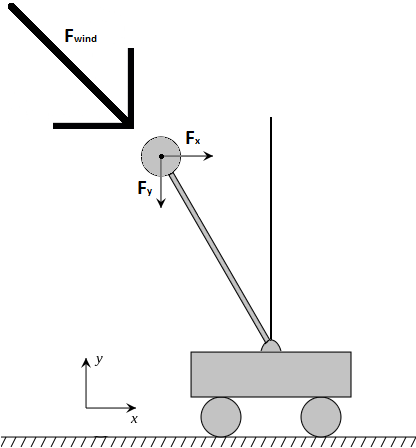
\includegraphics[width = 200pt]{WindForce} 
		\caption{\textit{Układ wahadła odwróconego na wózku w obecności siły wiatru}}
		\label{WindForce}
\end{figure}

Uzyskane siły $F_x$ i $F_y$ uwzględnione zostały jako dodatkowe oddziaływania względem modelu podstawowego. Aby wyznaczyć ich wpływ na dynamikę układu przeprowadzono rozważania analogiczne do tych, przedstawionych w sekcji \ref{MathModel}. W rezultacie ustalono poprawkę, która będzie doliczana wyłącznie wtedy, gdy do układu wprowadzone zostanie zakłócenie. Poszczególne wzory umieszczono w tabeli \ref{table:Noises}.

\begin{table}[H]
\begin{center}
\begin{tabular}{|c|c|}
  \hline 
  Element równania stanu & Zakłócenie \\
  \hline
  Prędkość liniowa $\frac{dx}{dt}$ & 0 \\
  \hline
  Prędkość kątowa $\frac{d\theta}{dt}$ & 0 \\
  \hline
  Przyspieszenie liniowe $\frac{d^2x}{dt^2}$ & $\frac{F_x - F_y\theta}{M}$ \\
  \hline
  Przyspieszenie kątowe $\frac{d^2\theta}{dt^2}$ & $\frac{(F_y\theta - F_x)(M + m)}{Mm}$ \\
  \hline
\end{tabular} 
\end{center}
\caption{Wzory na wyznaczenie poprawki związanej z zakłóceniem układu}
\label{table:Noises}
\end{table}

Omówiony model zakłóceń dotyczy pojedynczej pętli obliczeń, w której kierunek i moc wiatru są ustalone. Obsługa całego przebiegu symulacji wymaga rozważenia pełnej charakterystyki siły wiatru, w szczególności zmienności jej kierunku. W projekcie przyjęto, że wektor kierunku wiatru generowany będzie losowo z podprzestrzeni spełniającej nierówność: $|z| < 0.5$, natomiast moc wiatru i tempo jego zmiany będą dowolnie sterowalnymi parametrami. Dodatkowo opracowano kilka metod zmiany kierunku wiatru:
\begin{itemize}
\item Skoki losowe - przez zadany czas wiatr wieje z określonego kierunku, następnie generowany jest nowy losowy kierunek.
\item Skoki naprzemienne - przez zadany czas wiatr wieje z określonego kierunku, następnie generowany jest nowy kierunek w taki sposób, by wektor kierunkowy należał do półprzestrzeni przeciwnej do tej, w której znajduje się obecnie wybrany kierunek.
\item Gładkie przejścia - generowane są dwa kierunki podobnie jak w skokach naprzemiennych, które oznaczane są jako kierunek początkowy i końcowy. W trakcie przebiegu symulacji kierunek wiatru wyznaczany jest jako interpolacja wspomnianych dwóch wektorów. W celu uzyskania gładkiej zmiany kierunku wykorzystano interpolację SLERP omówioną w sekcji \ref{SLERP}. 
\end{itemize}

\subsection{Wprowadzenie trajektorii ruchu}
Zbudowany w dotychczasowy sposób system umożliwia stabilizację wahadła z uwzględnieniem zewnętrznych zakłóceń. Jednakże istotą projektu było przeniesienie układu do świata trójwymiarowego i swobodne poruszanie modelem po płaszczyźnie. Aby zapewnić ten warunek niezbędne jest rozszerzenie zagadnienia stabilizacji o zarządzanie pozycją wózka. Podobnie jak w przypadku regulacji kąta, zagadnienie można rozpatrywać w sytuacji dwuwymiarowej, ze względu na niezależne działanie podukładów. Ustalając pewne położenie $x$ jako punkt docelowy oraz $x_0$ jako miejsce startu problem można określić jako stabilizację układu w punkcie $x$ przy równoczesnym zadbaniu o utrzymanie wahadła w bezpiecznym wychyleniu. Ze względu na konieczność przebycia drogi $x - x_0$ przez pewien czas wahadło musi opuścić niestabilny punkt równowagi tak, by pokierować wózek do celu za pomocą wygenerowanej siły. Ponadto należy zwrócić uwagę na fakt, że wychylenie wahadła w kierunku docelowego punktu nie zapewni bezpośredniego ruchu podstawy w pożądaną stronę. Układ wykona kompensację wychylenia poprzez przesunięcie wózka w stronę przeciwną do zamierzonej i dopiero po pewnym czasie zacznie poruszać się z powrotem w pożądanym kierunku. 

Postawione komplikacje zmuszają do zastosowania odpowiedniego narzędzia umożliwiającego równoczesną kontrolę zachowania wahadła i wózka. W realizowanym projekcie skorzystano z podwójnego regulatora PID, którego charakterystykę przedstawiono w sekcji \ref{DoublePID}. Wybrany regulator możne być zaimplementowany na wiele sposobów. Autor pracy wybrał trzy metody, które zostały poddane gruntownym badaniom:
\begin{itemize}
\item Podwójny regulator równoległy (dla kąta: PID, dla pozycji: PD).
\item Zmodyfikowany podwójny regulator równoległy (dla kąta i pozycji: PD).
\item Podwójny regulator kaskadowy (dla kąta: PID, dla pozycji PD).
\end{itemize}

Pożądana wersja kontrolera powinna w możliwie najkrótszym czasie ustabilizować pozycję wózka w zadanym punkcie docelowym, nie doprowadzając do utraty kontroli nad wahadłem. Porównanie rozwiązań zostało przedstawione w rozdziale poświęconym testom. 

Dysponując sterowaniem pozwalającym na swobodny ruch układu do zadanego punktu można podjąć próbę zadania pełnej trajektorii ruchu. W fazie planowania projektu przyjęto, że trajektoria będzie składać się z ciągu dwuwymiarowych punktów kontrolnych zapisanych w pliku.

Przykładowa trajektoria zbudowana ze 100 punktów kontrolnych (z zaznaczonym ruchem wykonanym przez układ) pokazana została na rysunku \ref{TrajectoryTrefoilKnot}.

\begin{figure}[H]
	\centering
		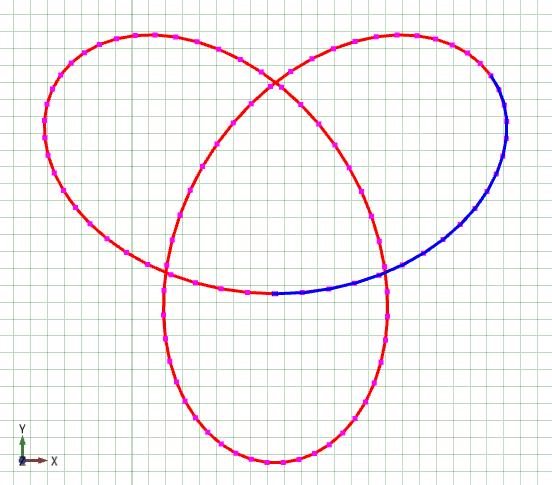
\includegraphics[width = 300pt]{TrajectoryTrefoilKnot} 
		\caption{\textit{Trajektoria ruchu w postaci płaskiego węzła koniczyny (ang. Trefoil Knot)}}
		\label{TrajectoryTrefoilKnot}
\end{figure}

Zadaniem symulatora jest wczytanie wybranej trajektorii i próba przeprowadzenia układu wzdłuż zadanej ścieżki ruchu z ustaloną dokładnością. Śledzenie trajektorii zrealizowano za pomocą następującego algorytmu:
\begin{enumerate}
\item Wczytanie i wyświetlenie zadanej trajektorii ruchu.
\item Wyznaczenie średniej odległości między punktami w celu kalibracji progów dokładności ruchu.
\item Ustawienie układu w punkcie startowym.
\item Dobór parametrów startowych (w tym dokładności realizacji ruchu).
\item W pętli po kolejnych punktach kontrolnych:
\begin{enumerate}
\item Wykonanie stabilizacji układu w danym punkcie kontrolnym wraz z graficznym zaznaczeniem zakreślonej przez układ faktycznej trajektorii ruchu.
\item Jeśli układ znajduje się w odpowiednio niedużej odległości od celu, zmiana punktu kontrolnego na następny.
W przypadku braku kolejnych punktów, zakończenie śledzenia ruchu. 
\end{enumerate}
\end{enumerate}

Ostatnim elementem związanym z omawianym problemem jest tworzenie trajektorii ruchu. Autor pracy przygotował kilka reprezentatywnych przykładów, które umożliwiają precyzyjne zbadanie różnych technik regulacji. Dodatkowo wykonana aplikacja pozwala na tworzenie dowolnych trajektorii ruchu poprzez podanie parametryzacji krzywej wraz z warunkami brzegowymi i pożądanej ilości punktów kontrolnych.

\subsection{Manualna kontrola nad układem}
W trakcie realizacji projektu autor pracy spostrzegł, że poruszanie układem jest zadaniem nietrywialnym i wymaga głębszego zrozumienia charakterystyki modelu. Użytkownik końcowy programu powinien móc przekonać się jak poszczególne zmiany stanu układu wpływają na ogólną dynamikę systemu i komplikację w jego sterowaniu. Aby spełnić to założenie przygotowano dodatkowy tryb pracy symulatora określony jako tryb gry. Moduł ten umożliwia zmianę wychylenia wahadła poprzez modyfikację wartości zadanej uchybu kąta odchylenia wahadła od pionu. W rezultacie użytkownik zyskuje narzędzie do manualnego poruszania układem. Wprowadzając dodatkowo trajektorię ruchu, użytkownik ma możliwość podjęcia próby przeprowadzenia wózka wzdłuż zadanej ścieżki. Po włączeniu modułu zakłóceń pochodzących od siły wiatru pojawia się problem manualnego utrzymania stałej pozycji wózka, na przekór działającemu zakłóceniu. Wszystkie wymienione elementy pozwalają doświadczalnie zbadać charakterystykę układu, stanowiąc przy okazji przyjemną zabawę.

\section{Algorytm pracy symulatora}
Głównym zadaniem symulatora jest wizualizacja mechaniki układu wahadła odwróconego na wózku w obecności różnych założeń zaprezentowanych w poprzednich sekcjach. Dodatkowo narzędzie pozwala na pełną konfigurację wszystkich kluczowych parametrów, zarówno samego układu, jak i całej symulacji. Ogólny przebieg pracy symulatora prezentuje poniższy algorytm:
\begin{enumerate}
\item Wybór trybu pracy między stabilizacją wahadła, śledzeniem trajektorii i trybem gry.
\item Konfiguracja opcji symulacji takich jak: typ regulatora, rodzaj zakłóceń, tryb wyświetlania.
\item Ustalenie parametrów początkowych systemu:
\begin{itemize}
\item Krok czasowy obliczeń.
\item Początkowe wychylenie wahadła w osiach O(X) i O(Y).
\item Długość wahadła.
\item Masa wahadła.
\item Masa wózka.
\end{itemize}
\item Określenie mocy i szybkości zmiany kierunku siły wiatru (modyfikowalne w trakcie trwania animacji).
\item Przygotowanie kontrolerów i uruchomienie symulacji dla zadanego środowiska.
\item W pętli czasowej do zatrzymania symulacji:
\begin{enumerate}
\item Pobranie aktualnego punktu kontrolnego (w przypadku trybu śledzenia trajektorii).
\item Pobranie aktualnego stanu wiatru (w przypadku włączenia zakłóceń).
\item Podanie do kontrolera napięcia na silniku uchybu kąta i pozycji.
\item Wyznaczenie napięcia regulującego, przekazanie wyniku do modułu obliczeniowego.
\item Wyznaczenie rozwiązań równań stanu dla dwuwymiarowych układów przy pomocy algorytmu Rungego-Kutty.
\item Wyznaczenie złożenia podukładów w model trójwymiarowy.
\item Aktualizacja wizualizacji, wykresów i czasu.
\end{enumerate}
\item Zakończenie symulacji, powrót do stanu początkowego.
\end{enumerate}

%% -------- chapter IV --------
\chapter{Testy i porównanie przyjętych rozwiązań}
\section{Założenia wstępne}
Testowanie poprawności działania jest niezbędnym elementem w procesie tworzenia oprogramowania symulacyjnego. Jedynie gruntowna seria prób sprawdzających wszystkie istotne funkcjonalności pozwala na stwierdzenie czy opracowane rozwiązanie daje akceptowalne wyniki i w rezultacie jest użyteczne dla użytkownika końcowego. Dodatkowo testy pozwalają na porównanie różnych strategi opracowanych w trakcie projektowania modelu systemu i wybór najlepszego zestawu rozwiązań. 

Autor pracy skupił się na zbadaniu ogólnej pracy symulatora w zależności od zadanej interakcji użytkownika, jak również wykorzystał fazę testów do analizy porównawczej kilku aspektów projektu, w szczególności:
\begin{itemize}
\item Stabilizacja układu za pomocą różnych metod regulacji.
\item Ruch układu po zadanej trajektorii przy użyciu poszczególnych wariantów regulatora podwójnego PID.
\item Wpływ parametrów początkowych na jakość stabilizacji.
\item Wpływ zakłóceń pochodzących od siły wiatru na zachowanie układu.
\end{itemize}

Każde z zagadnień zostało dokładnie omówione w poszczególnych sekcjach wraz z prezentacją wykresów i wypracowanych wniosków. W celach porównawczych przygotowano zestawy wykresów obejmujące:
\begin{itemize}
\item Wykres zależności uchybu (kąta bądź pozycji) od czasu.
\item Wykres zależności napięcia na silniku od czasu.
\item Wykres trajektorii ruchu (dla trybu śledzenia trajektorii).
\end{itemize}

Pojedynczy wykres zawiera dane dostarczane przez poszczególne układy dwuwymiarowe. W celu uniknięcia nieczytelności, każdy zestaw danych zaznaczony został innym kolorem.

Konfiguracja parametrów początkowych przeprowadzona została zgodnie z przyjętymi wartościami nominalnymi przedstawionymi w tabeli \ref{table:NominalParameters}. Pozostałe nieokreślone parametry ustawiono na następujące wartości:
\begin{itemize}
\item Odstęp czasu: 0.01 s.
\item Wychylenie początkowe w osi O(X): 0.8 rad.
\item Wychylenie początkowe w osi O(Y): -0.4 rad.
\end{itemize}

\section{Stabilizacja układu}
\subsubsection{Brak sterowania}
Brak jakiegokolwiek narzędzia sterującego powoduje, że symulacja układu ogranicza się do wizualizacji zachowania wahadła i wózka w zależności od wychylenia wahadła. Nawet niewielkie zaburzenia kąta powodują, że wahadło opuszcza niestabilny punkt równowagi o opada na wózek. W tym czasie podstawa wykonuje ruch w stronę przeciwną do kierunku wychylenia wahadła. Omawiana sytuacja została pokazana na rysunku \ref{figure:ModelWithoutControl}.

\begin{figure}[H]
	\centering
		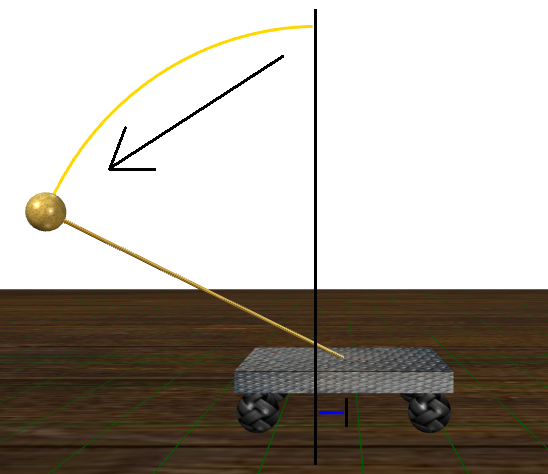
\includegraphics[width = 250pt]{ModelWithoutControl} 
		\caption{\textit{Wizualizacja zachowania układu w przypadku braku sterowania}}
		\label{figure:ModelWithoutControl}
\end{figure}

\subsubsection{Sterowanie niezależne od uchybu}
Przeprowadzono sprawdzenie zachowania układu w obecności regulatora napięcia na silniku sterującym platformą. W pierwszym przypadku zastosowano sterowanie niezależne od uchybu w celu zbadania reakcji układu na dowolny moduł kontrolujący. Dla uproszczenia sytuacji zaniechano wstępnego wychylania wahadła. Wyniki testu pokazano na wykresach: \ref{plot:RandomEV}, \ref{plot:RandomCE}, \ref{plot:SinusoidalEV}, \ref{plot:SinusoidalCE}.

\begin{figure}[H]
	\centering
		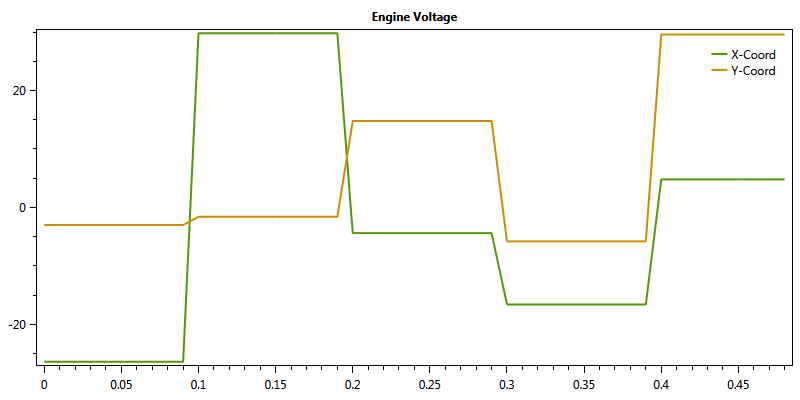
\includegraphics[width = 350pt]{RandomEV} 
		\caption{\textit{Sterowanie losowym napięciem: wykres zależności napięcia na silniku od czasu}}
		\label{plot:RandomEV}
\end{figure}

\begin{figure}[H]
	\centering
		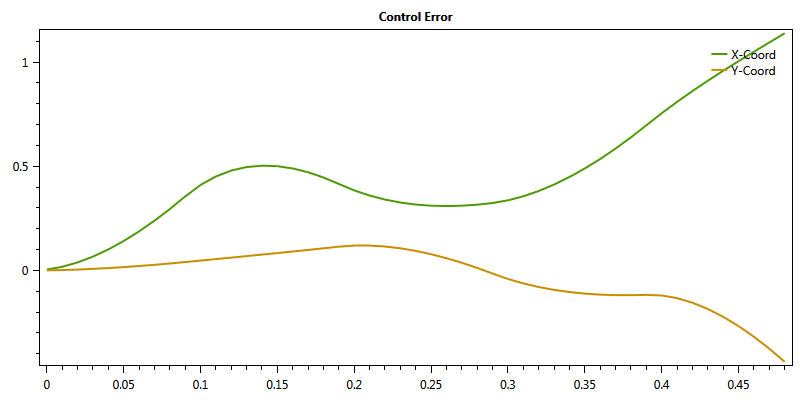
\includegraphics[width = 350pt]{RandomCE} 
		\caption{\textit{Sterowanie losowym napięciem: wykres zależności uchybu kąta od czasu}}
		\label{plot:RandomCE}
\end{figure}

\begin{figure}[H]
	\centering
		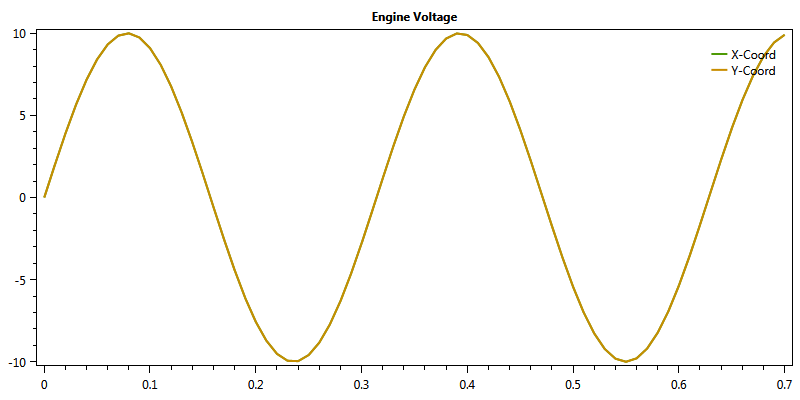
\includegraphics[width = 350pt]{SinusoidalEV} 
		\caption{\textit{Sterowanie sinusoidalnym napięciem: wykres zależności napięcia na silniku od czasu}}
		\label{plot:SinusoidalEV}
\end{figure}

\begin{figure}[H]
	\centering
		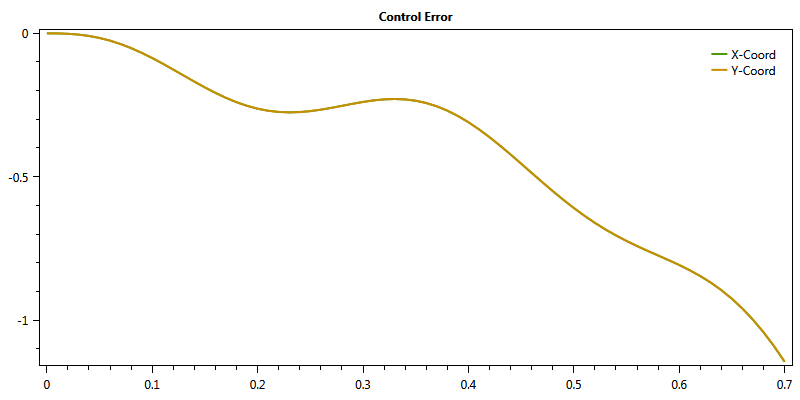
\includegraphics[width = 350pt]{SinusoidalCE} 
		\caption{\textit{Sterowanie sinusoidalnym napięciem: wykres zależności uchybu kąta od czasu}}
		\label{plot:SinusoidalCE}
\end{figure}

Zgodnie z oczekiwaniami przyjęta regulacja nie spowodowała utrzymania wahadła w punkcie równowagi. Już po krótkim czasie trwania symulacji wahadło opada na platformę uniemożliwiając dalsze sterowanie. Wykonany test jednoznacznie stwierdził, że zadanie stabilizacji wahadła może być zrealizowane wyłącznie przez odpowiednio przygotowany kontroler.

\subsubsection{Sterowanie regulatorem PID}
Kolejny test dotyczył pracy regulatora PID, dedykowanego narzędzia służącego do stabilizacji układu. Przed przystąpieniem do wykonania symulacji należało zadbać o poprawny dobór nastaw regulatora. Autor pracy wykorzystał w tym celu parametry zaproponowane w pracy \cite{JTJT}. Są to:
\begin{itemize}
\item $K_p = -50.8$
\item $T_i = 7.26$
\item $T_d = 0.24$
\end{itemize}

W celu weryfikacji ich poprawności przeprowadzono testy jakości stabilizacji dla pewnych modyfikacji poszczególnych wartości. Wyniki pokazały, że nie udało się uzyskać lepszej jakości dla innego zestawu parametrów niż podane.

Dla tak przygotowanego środowiska przeprowadzono test stabilizacji analogiczny do dwóch poprzednich przykładów. Wyniki przedstawiono na wykresach \ref{plot:PIDEV} oraz  \ref{plot:PIDCE}.

\begin{figure}[H]
	\centering
		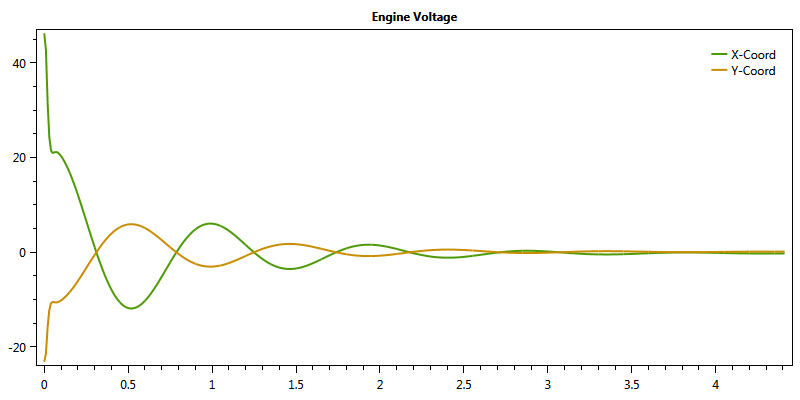
\includegraphics[width = 350pt]{PIDEV} 
		\caption{\textit{Sterowanie poprzez regulator PID: wykres zależności napięcia na silniku od czasu}}
		\label{plot:PIDEV}
\end{figure}

\begin{figure}[H]
	\centering
		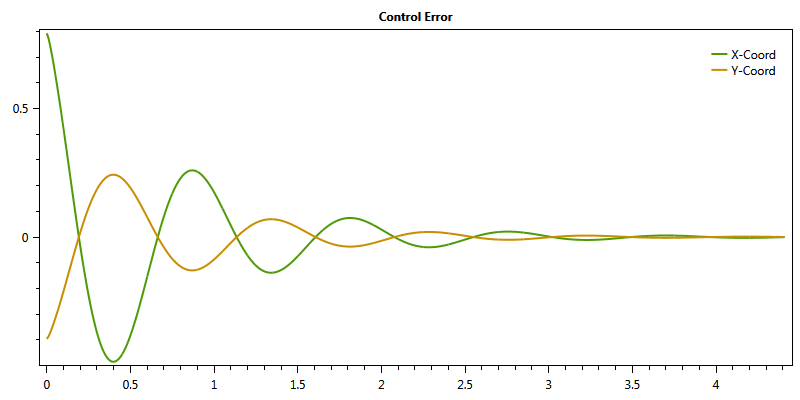
\includegraphics[width = 350pt]{PIDCE} 
		\caption{\textit{Sterowanie poprzez regulator PID: wykres zależności uchybu kąta od czasu}}
		\label{plot:PIDCE}
\end{figure}

Charakterystyka wykresów jednoznacznie wskazuje na stopniowe wygaszanie wychylenia wahadła wraz z narastającym czasem. Regulator PID podając odpowiednie napięcie do układu kompensuje ruch obrotowy wahadła przez ruch postępowy wózka. W ostateczności wahadło stabilizuje swoje wychylenie w obydwu osiach układu.

\section{Ruch po trajektorii}
\subsection{Założenia}
\label{Reqs}
Kolejnym zagadnieniem wymagającym gruntownych testów była ocena jakości realizowania trajektorii ruchu przez poszczególne układy sterujące. W celu uzyskania efektu poruszania wykorzystano układ podwójnego regulatora PID. W oparciu o literaturę opracowano współczynniki nastaw poszczególnych kontrolerów. W przypadku regulatora kąta pozostawiono wartości opracowane w poprzedniej sekcji. Dla regulatora pozycji po zbadaniu transmitancji układu i stwierdzeniu jego całkującego charakteru, zdecydowano się na skorzystanie z regulatora w wersji PD. Aby to osiągnąć przyjęto następujące nastawy:
\begin{itemize}
\item Dla regulatora kaskadowego:
\begin{itemize}
\item $K_p = 0.05$,
\item $T_i = \infty$,
\item $T_d = 0.7$.
\end{itemize}
\item Dla regulatora równoległego:
\begin{itemize}
\item $K_p = 6$,
\item $T_i = \infty$,
\item $T_d = 1.5$.
\end{itemize}
\end{itemize}

W trakcie przeprowadzania pierwszych testów symulacji autor pracy zwrócił uwagę na negatywny wpływ członu całkującego regulatora kąta na szybkość wykonywania ruchu po trajektorii. Po zastanowieniu się nad istotą problemu, włączono do porównania trzeci układ sterowania, w którym zaniechano użycia wspomnianego członu.


W celu uzyskania wiarygodnych wyników testy przeprowadzono dla trzech reprezentatywnych przypadków trajektorii:
\begin{itemize}
\item Trajektoria odcinka - możliwość sprawdzenia stabilizacji układu w pojedynczym punkcie kontrolnym.
\item Trajektoria węzła koniczynowego (pokazanego na rysunku \ref{TrajectoryTrefoilKnot}) - chęć zbadania jakości ruchu w przypadku nietrywialnej, złożonej trajektorii.
\item Trajektoria krzyża - ocena zachowania układu wobec przypadku szczególnego, w którym kolejne punkty kontrolne są od siebie odległe i tworzą wzajemnie kąty proste.
\end{itemize}

Głównymi kryteriami porównawczymi były: 
\begin{itemize}
\item Dokładność odzwierciedlenia trajektorii.
\item Czas wykonania ruchu.
\item Stabilność wahadła w czasie transportu.
\item Charakterystyka napięcia na silniku.
\end{itemize}

\subsection{Trajektoria prosta}
W pierwszej kolejności zbadano zachowanie układu dla prostej trajektorii odcinka. Wózek ustawiony został w początku układu współrzędnych i jego zadaniem było przemieszczenie się do punktu $(2.5,-2.5)$.

\subsubsection{Podwójny regulator równoległy}
Wykresy napięcia na silniku oraz uchybów pozycji i kąta dla podwójnego regulatora równoległego przedstawiono na wykresach \ref{plot:LinePIDEV}, \ref{plot:LinePIDCEP} i \ref{plot:LinePIDCEA}.

\begin{figure}[H]
	\centering
		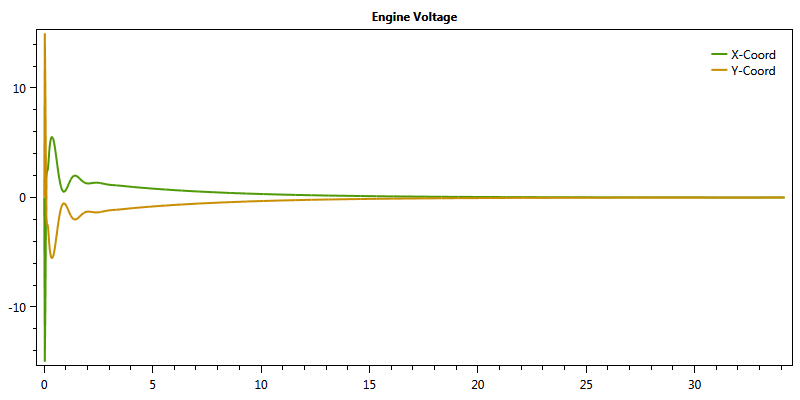
\includegraphics[width = 350pt]{LinePIDEV} 
		\caption{\textit{Stabilizacja w punkcie kontrolnym za pomocą podwójnego regulatora równoległego: wykres zależności napięcia na silniku od czasu}}
		\label{plot:LinePIDEV}
\end{figure}

\begin{figure}[H]
	\centering
		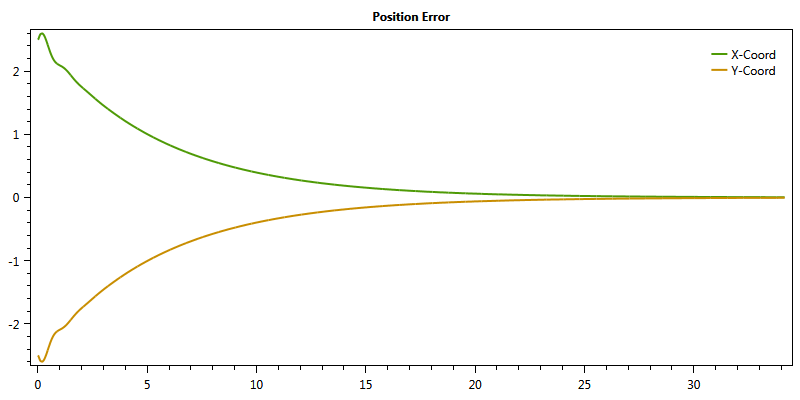
\includegraphics[width = 350pt]{LinePIDCEP} 
		\caption{\textit{Stabilizacja w punkcie kontrolnym za pomocą podwójnego regulatora równoległego: wykres zależności uchybu pozycji od czasu}}
		\label{plot:LinePIDCEP}
\end{figure}

\begin{figure}[H]
	\centering
		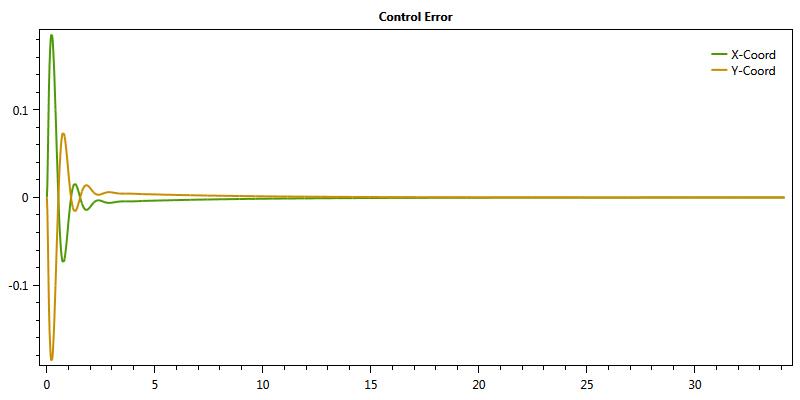
\includegraphics[width = 350pt]{LinePIDCEA} 
		\caption{\textit{Stabilizacja w punkcie kontrolnym za pomocą podwójnego regulatora równoległego: wykres zależności uchybu kąta od czasu}}
		\label{plot:LinePIDCEA}
\end{figure}

Wykresy jednoznacznie wskazują na poprawną stabilizację układu w docelowej lokacji. Kontroler dba o utrzymanie wahadła w bezpiecznym wychyleniu, przesuwając się powoli w kierunku punktu kontrolnego. Istotną cechą układu jest asymptotyczne zbieganie do poprawnej pozycji, toteż nie ma potrzeby wykonywania poprawki po osiągnięciu finalnej pozycji. Generowane napięcie na silniku jest akceptowalne. Testy ukazują, że jedyną wadą sterowania jest zbyt długi czas trwania ruchu (około 30 sekund do pełnej stabilizacji).

\subsubsection{Zmodyfikowany podwójny regulator równoległy}
Wykresy napięcia na silniku oraz uchybów pozycji i kąta dla zmodyfikowanego podwójnego regulatora równoległego przedstawiono na wykresach \ref{plot:LinePDEV}, \ref{plot:LinePDCEP} i \ref{plot:LinePDCEA}.

\begin{figure}[H]
	\centering
		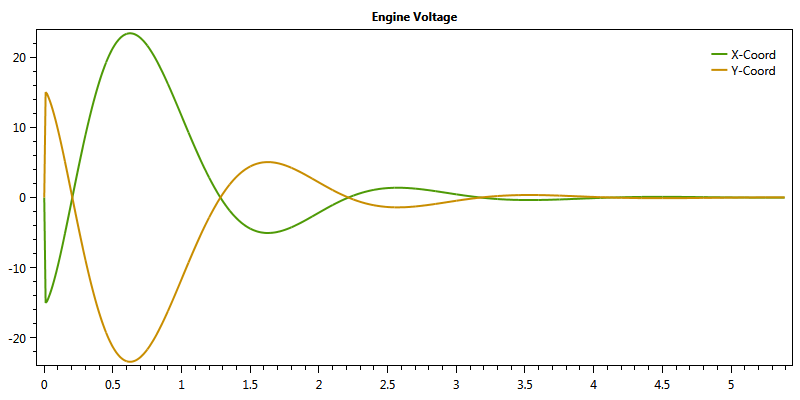
\includegraphics[width = 350pt]{LinePDEV} 
		\caption{\textit{Stabilizacja w punkcie kontrolnym za pomocą zmodyfikowanego podwójnego regulatora równoległego: wykres zależności napięcia na silniku od czasu}}
		\label{plot:LinePDEV}
\end{figure}

\begin{figure}[H]
	\centering
		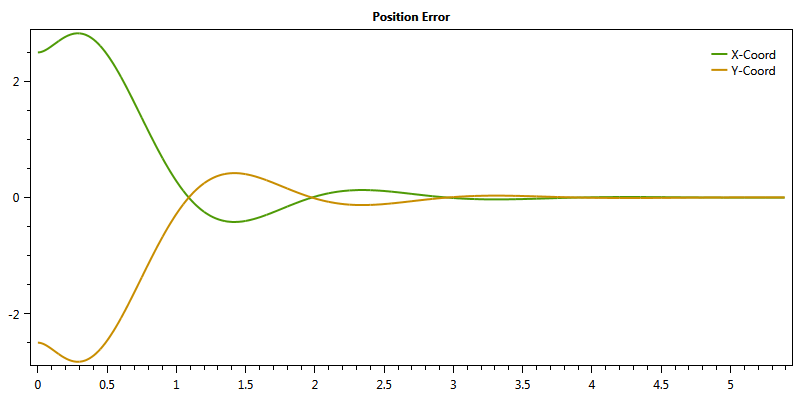
\includegraphics[width = 350pt]{LinePDCEP} 
		\caption{\textit{Stabilizacja w punkcie kontrolnym za pomocą zmodyfikowanego podwójnego regulatora równoległego: wykres zależności uchybu pozycji od czasu}}
		\label{plot:LinePDCEP}
\end{figure}

\begin{figure}[H]
	\centering
		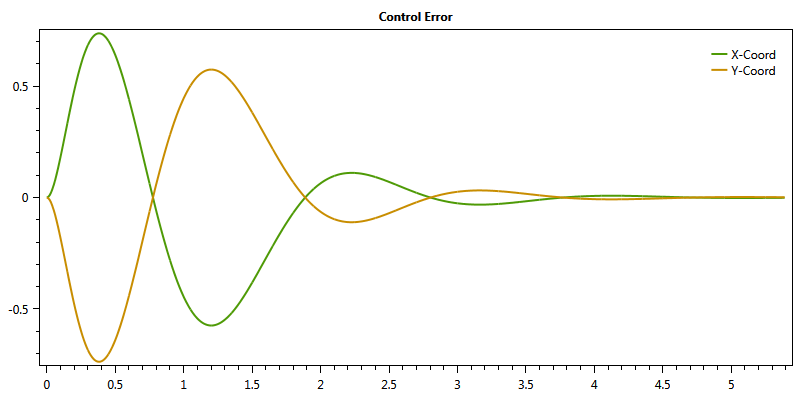
\includegraphics[width = 350pt]{LinePDCEA} 
		\caption{\textit{Stabilizacja w punkcie kontrolnym za pomocą zmodyfikowanego podwójnego regulatora równoległego: wykres zależności uchybu kąta od czasu}}
		\label{plot:LinePDCEA}
\end{figure}

W przypadku układu sterowania z wyłączonym modułem całkującym dla regulacji kąta stabilizacja realizowana jest na podobnym poziomie jak w niezmodyfikowanym modelu. System cechują dużo większe wychylenia wahadła, jednakże zauważalna jest poprawa czasu wykonywania ruchu (redukcja do 5 sekund). Układ przy osiąganiu punktu docelowego wymaga wykonania drobnej poprawki pozycji. Charakterystyka napięcia wskazuje na większy udział napędu silnika w dynamikę układu. 

\subsubsection{Podwójny regulator kaskadowy}
Wykresy napięcia na silniku oraz uchybów pozycji i kąta dla podwójnego regulatora kaskadowego przedstawiono na wykresach \ref{plot:LineCasPIDEV}, \ref{plot:LineCasPIDCEP} i \ref{plot:LineCasPIDCEA}.

\begin{figure}[H]
	\centering
		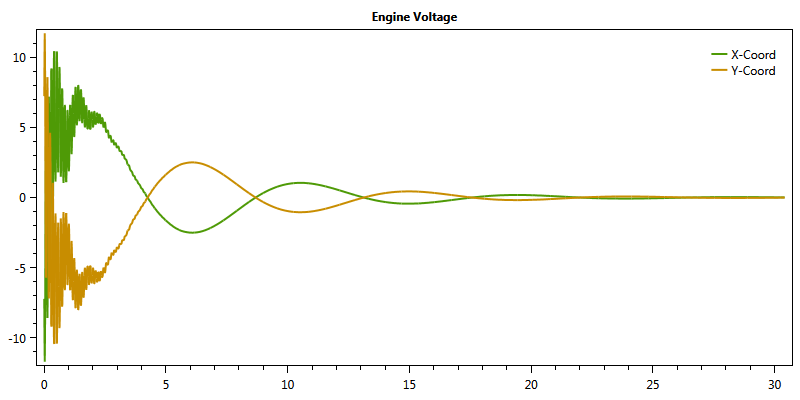
\includegraphics[width = 350pt]{LineCasPIDEV} 
		\caption{\textit{Stabilizacja w punkcie kontrolnym za pomocą podwójnego regulatora kaskadowego: wykres zależności napięcia na silniku od czasu}}
		\label{plot:LineCasPIDEV}
\end{figure}

\begin{figure}[H]
	\centering
		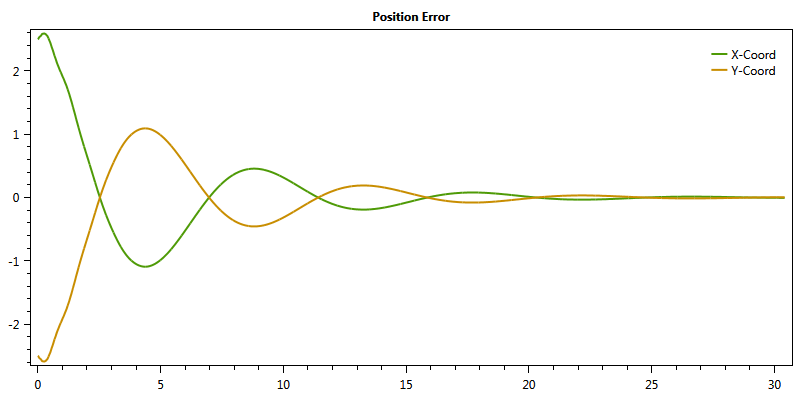
\includegraphics[width = 350pt]{LineCasPIDCEP} 
		\caption{\textit{Stabilizacja w punkcie kontrolnym za pomocą podwójnego regulatora kaskadowego: wykres zależności uchybu pozycji od czasu}}
		\label{plot:LineCasPIDCEP}
\end{figure}

\begin{figure}[H]
	\centering
		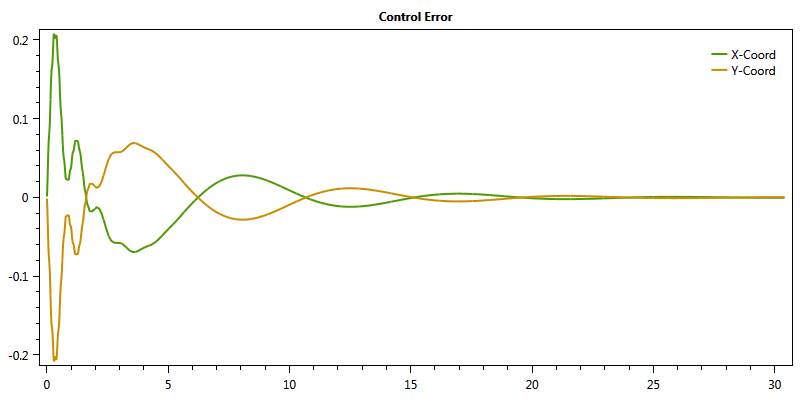
\includegraphics[width = 350pt]{LineCasPIDCEA} 
		\caption{\textit{Stabilizacja w punkcie kontrolnym za pomocą podwójnego regulatora kaskadowego: wykres zależności uchybu kąta od czasu}}
		\label{plot:LineCasPIDCEA}
\end{figure}

Podobnie jak w przypadku dwóch poprzednich sterowników, regulator kaskadowy potrafi ustabilizować układ w zadanym położeniu. Czas realizacji zadania jest zbliżony do niezmodyfikowanego sterowania równoległego. W trakcie trwania ruchu daje się zauważyć częste obustronne wychylenia wahadła. Po osiągnięciu pozycji docelowej układ wykonuje dalszy ruch w zadanym kierunku, przez co niezbędna jest kilkukrotna poprawka powrotna pozycji. Niestety charakterystyka napięcia na silniku wskazuje na nieregularne (często skokowe) wartości napięcia, szczególnie w początkowej fazie ruchu. Zachowanie to jest nieakceptowalne w przypadku rozwiązania wdrażanego do rzeczywistego układu. 

\subsection{Trajektoria złożona}
Celem finalnym symulatora było śledzenie trajektorii złożonej z wielu punktów kontrolnych. Algorytm pracy transportera wymagał osiągnięcia przez układ kolejnych punktów kontrolnych, nie zwracając uwagi na stabilizację wahadła w konkretnym punkcie, tzn. po dotarciu do określonego miejsca, układ ma natychmiastowo przystąpić do ruchu do kolejnej lokacji. 

Przetestowanie funkcjonalności oparto na dwóch przykładach. Jeden z nich obejmował transport układu po gładkim łuku węzła koniczynowego. Jest to typowy odcinek trajektorii, który system powinien wykonać bez większych trudności. Drugim przykładem była trajektoria krzyża. Symulator w założeniu nie obejmował tego typu trajektorii, jednakże wykorzystanie go pozwala na porównanie cech poszczególnych kontrolerów. 

\subsubsection{Fragment trajektorii węzła koniczynowego}
Podobnie jak w przypadku prostej trajektorii układ został umieszczony na miejscu startowym, po czym symulator powinien przystąpić do przesuwania układu wzdłuż zadanej trajektorii. Podczas trwania symulacji na płaszczyźnie ruchu zaznaczano kolejne pozycje wózka, śledząc równocześnie zachowanie wahadła. Trajektorię wyrysowaną przez obydwie wersje podwójnego regulatora równoległego pokazano na rysunku \ref{TrajectoryTrefoilKnotGood}. Trajektorię pochodzącą od podwójnego regulatora kaskadowego przedstawia ilustracja \ref{TrajectoryTrefoilKnotWrong}.

\begin{figure}[H]
	\centering
		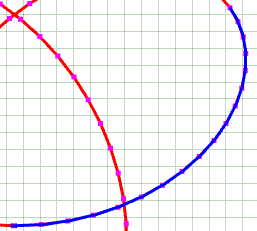
\includegraphics[width = 200pt]{TrajectoryTrefoilKnotGood} 
		\caption{\textit{Ruch układu śledzącego trajektorię węzła koniczynowego w przypadku sterowania podwójnym regulatorem równoległym}}
		\label{TrajectoryTrefoilKnotGood}
\end{figure}

\begin{figure}[H]
	\centering
		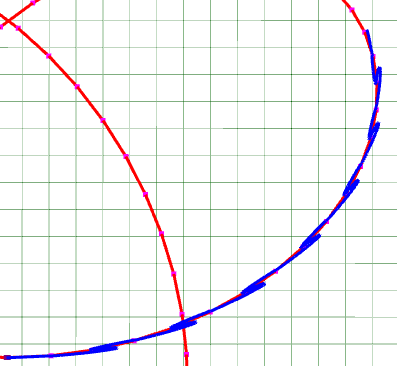
\includegraphics[width = 200pt]{TrajectoryTrefoilKnotWrong} 
		\caption{\textit{Ruch układu śledzącego trajektorię węzła koniczynowego w przypadku sterowania podwójnym regulatorem kaskadowym}}
		\label{TrajectoryTrefoilKnotWrong}
\end{figure}

Zarówno podwójny regulator równoległy, jak i jego zmodyfikowana wersja poradziły sobie z zadanym ruchem bez większych problemów. Dodatkowym atutem drugiego z nich był znacznie mniejszy czas potrzebny do wykonania przesunięcia do celu. Niestety w przypadku regulatora kaskadowego przyjęta technika pokonywania drogi okazała się barierą do wykonania poprawnego ruchu. Regulator ten ze względu na długi czas stabilizacji pozycji często gubił odpowiednią trajektorię i był zmuszony wracać do punktu kontrolnego.

Przeprowadzono dodatkowo ocenę wykresów parametrów sterowania umieszczonych w dodatku \ref{appenix:A}. Zgodnie z zachowaniem układu obserwowanym w wizualizacji wykresy napięcia na silniku oraz uchybu kąta dla regulatora kaskadowego przedstawiają problemy w ustabilizowaniu układu i dynamiczne zmiany napięcia, które negatywnie wpływają na pracę systemu. Dla podwójnego regulatora równoległego można dostrzec drobne wychylenia inicjujące ruch, gaszone powoli poprzez sterowanie silnikiem. W przypadku zmodyfikowanego regulatora równoległego wykresy prezentują się najbardziej obiecująco. Przejścia między kolejnymi fazami są dość gładkie, a poziomy wychylenia wahadła akceptowalne.

Badaniu poddano również trajektorie: okręgu, Lemniskaty Bernoulliego oraz krzywej sinusoidalnej. Uzyskane rezultaty w pełni odzwierciedlają wyprowadzone wnioski. Wobec powyższego należy przyjąć, że dla zadania ruchu po gładkiej trajektorii należy wykorzystać zmodyfikowany podwójny regulator równoległy.

\subsubsection{Trajektoria krzyża}
W opozycji do przykładów z poprzedniej sekcji przygotowano jeszcze jeden przykład testowy, w którym trajektoria składa się z odległych od siebie punktów kontrolnych tworzących kolejno kąty proste. Zadanie to zostało wybrane w celu zbadania, jak układ poradzi sobie w sytuacji, gdy użytkownik wymaga gwałtownego skrętu transportera (np. w przypadku dojechania do przeszkody). Wyniki testów przedstawiono w formie wykresów trajektorii realizowanej przez wózek: \ref{TrajectoryCrossParallel}, \ref{TrajectoryCrossPD}, \ref{TrajectoryCrossCascade}.

\begin{figure}[H]
	\centering
		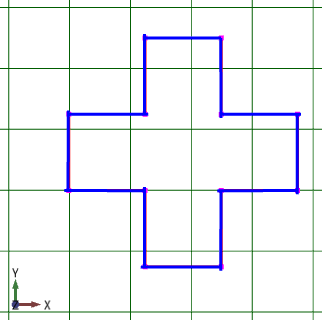
\includegraphics[width = 200pt]{TrajectoryCrossParallel} 
		\caption{\textit{Ruch układu śledzącego trajektorię krzyża w przypadku sterowania podwójnym regulatorem równoległym}}
		\label{TrajectoryCrossParallel}
\end{figure}

\begin{figure}[H]
	\centering
		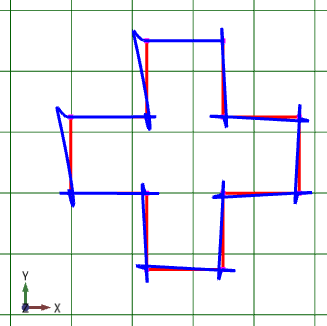
\includegraphics[width = 200pt]{TrajectoryCrossPD} 
		\caption{\textit{Ruch układu śledzącego trajektorię krzyża w przypadku sterowania zmodyfikowanym podwójnym regulatorem równoległym}}
		\label{TrajectoryCrossPD}
\end{figure}

\begin{figure}[H]
	\centering
		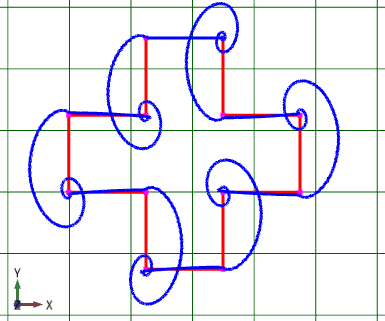
\includegraphics[width = 200pt]{TrajectoryCrossCascade} 
		\caption{\textit{Ruch układu śledzącego trajektorię krzyża w przypadku sterowania podwójnym regulatorem kaskadowym}}
		\label{TrajectoryCrossCascade}
\end{figure}

Zgodnie z początkowymi przypuszczeniami, jedynie podwójny regulator równoległy był w stanie w pełni odtworzyć zadaną trajektorię. Rezultat ten bierze się z faktu, że wspomniany kontroler jako jedyny zbiega dokładnie do docelowego punktu, bez konieczności wykonywania poprawki wstecznej. W przypadku pozostałych regulatorów trudność zadania sprawiła, że w pewnych miejscach regulator nie był w stanie w pełni ustabilizować układu, a był zmuszony do realizowania dalszego ruchu. Gdyby przyjęta została inna koncepcja ruchu, prawdopodobnie uzyskane przemieszczenia byłyby dokładniejsze, jednakże w wybranym rozwiązaniu postawiono na ciągłość ruchu.


\section{Wpływ parametrów układu}
W celu określenia wpływu parametrów początkowych układu na szybkość stabilizacji za pomocą regulatora PID przeprowadzono serię testów porównawczych. Najpierw ustawiono konfigurację systemu w sposób opisany w sekcji \ref{Reqs}. Następnie modyfikowano wartości poszczególnych parametrów i sprawdzano po jakim czasie wychylenie wahadła i jego prędkość kątowa będą odpowiednio małe. Test ten zapewnił jednoznaczne określenie czy układ ustabilizował się w punkcie równowagi. 

\newpage
\subsubsection{Masa wózka}
Charakterystykę wpływu masy wózka na czas trwania stabilizacji przedstawiono na wykresie \ref{plot:CartMassQuality}.

\begin{figure}[H]
	\centering
		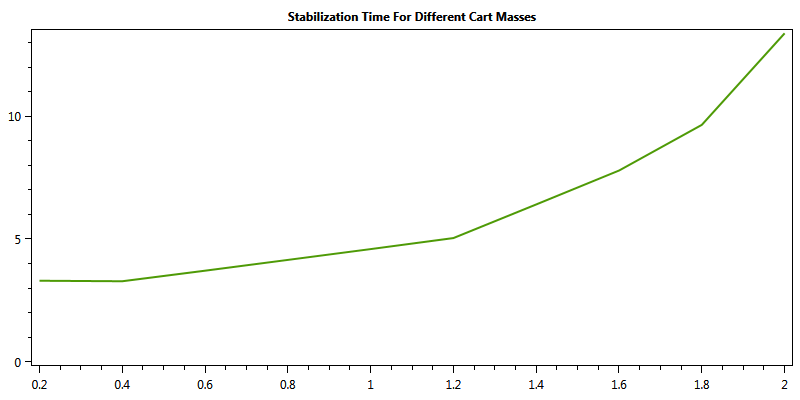
\includegraphics[width = 350pt]{CartMassQuality} 
		\caption{\textit{Wykres wpływu masy wózka na czas trwania stabilizacji układu}}
		\label{plot:CartMassQuality}
\end{figure}

Wraz ze zwiększaniem masy podstawy czas regulacji ulegał znacznemu wydłużeniu. Dla masy 1 kg stabilizacja trwała około 5 sekund, a dla zdwojonej masy, czas ten był niemalże potrojony. Wykres jednoznacznie sugeruje, że masa wózka jest bardzo istotnym czynnikiem wpływającym na stabilizację. Dodatkowe testy przeprowadzone dla mas powyżej 3 kg pokazały, że regulator nie jest już w stanie poradzić sobie ze stabilizacją. Uzyskane wyniki są zgodne z oczekiwaniami, gdyż sterowanie cięższym wózkiem wymaga coraz więcej mocy od silnika napędowego, a wykonanie jakiegokolwiek ruchu platformą staje się coraz trudniejsze. Ponadto masa wózka jest istotnym parametrem przy wyznaczaniu sterowania układem w równaniach ruchu. 

\newpage
\subsubsection{Masa wahadła}
Charakterystykę wpływu masy wahadła na czas trwania stabilizacji przedstawiono na wykresie \ref{plot:PendulumMassQuality}.
\begin{figure}[H]
	\centering
		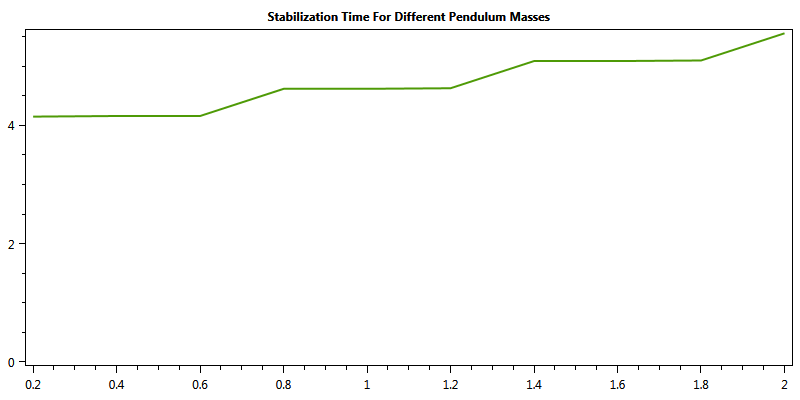
\includegraphics[width = 350pt]{PendulumMassQuality} 
		\caption{\textit{Wykres wpływu masy wahadła na czas trwania stabilizacji układu}}
		\label{plot:PendulumMassQuality}
\end{figure}

W przeciwieństwie do masy wózka, masa wahadła nie wpływa w aż tak znaczącym stopniu na jakość stabilizacji układu. Wykres wskazuje na przyrost czasu wraz ze wzrostem masy, jednakże regulator jest w stanie kompensować wychylenia nawet w przypadku znacznej masy wahadła. Charakterystykę tę można powiązać z zależnością wartości momentu siły przyłożonego do wahadła od jego masy, co przekłada się na większe przyspieszenie kątowe i większe wychylenia wahadła.

\newpage
\subsubsection{Długość wahadła}
Charakterystykę wpływu długości wahadła na czas trwania stabilizacji przedstawiono na wykresie \ref{plot:PendulumLengthQuality}.
\begin{figure}[H]
	\centering
		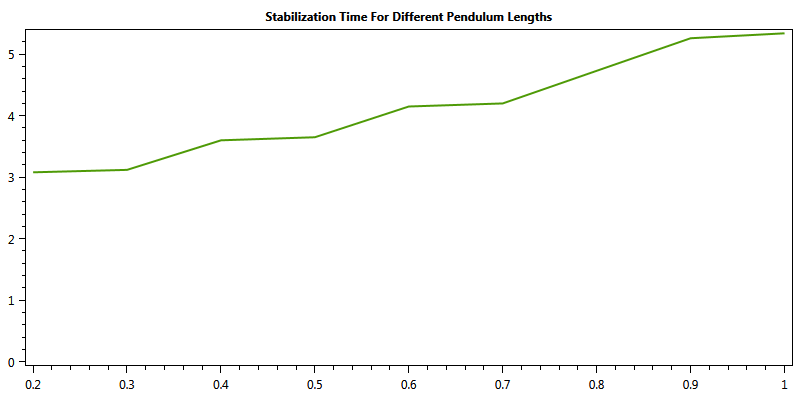
\includegraphics[width = 350pt]{PendulumLengthQuality} 
		\caption{\textit{Wykres wpływu długości wahadła na czas trwania stabilizacji układu}}
		\label{plot:PendulumLengthQuality}
\end{figure}

Podobnie jak dla masy wahadła jego długość wpływa na stabilizację w sposób liniowo rosnący. Współczynnik kierunkowy prostej przybliżającej wykres jest większy niż dla poprzedniego wykresu, toteż można wnioskować, że długość wahadła ma większy wpływ na jakość regulacji układu. Obserwacja ta jest zgodna z intuicją, gdyż trudniej jest utrzymać poprawne wychylenie obiektu, który jest dłuższy. Ponadto długość wahadła jest istotnym parametrem przy wyznaczaniu sterowania układem w równaniach ruchu. 

\newpage
\subsubsection{Wychylenie początkowe}
Charakterystykę wpływu początkowego wychylenia wahadła na czas trwania stabilizacji przedstawiono na wykresie \ref{plot:PendulumAngleQuality}.
\begin{figure}[H]
	\centering
		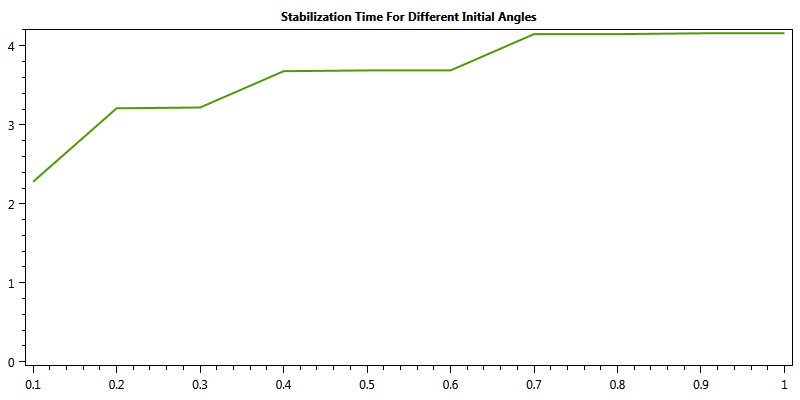
\includegraphics[width = 350pt]{PendulumAngleQuality} 
		\caption{\textit{Wykres wpływu początkowego wychylenia wahadła na czas trwania stabilizacji układu}}
		\label{plot:PendulumAngleQuality}
\end{figure}

Zgodnie z oczekiwaniami większe wychylenie początkowe wymaga dłuższego czasu stabilizacji. Ciekawym spostrzeżeniem jest fakt, iż wraz ze wzrostem wychylenia jego wpływ na jakość stabilizacji jest coraz mniejszy. Dla kątów powyżej 0.7 rad różnica ta jest minimalna.

\section{Wpływ zakłóceń pochodzących od siły wiatru}
Ostatnim zagadnieniem poddanym testom był wpływ zakłóceń na pracę układu. Ze względu na losowy charakter siły wiatru nie skupiano się na dokładnej charakterystyce zachowania układu, a jedynie na zmianach zachodzących podczas modyfikacji mocy i kierunku zakłócenia. Badania przeprowadzono dla stabilizacji zmodyfikowanym regulatorem podwójnym równoległym z pozycją docelową w początku układu współrzędnych (wyniki umieszczone na wykresach \ref{plot:WindPDEV}, \ref{plot:WindPDCEP}, \ref{plot:WindPDCEA}) oraz prostym regulatorem PID (wykresy zaprezentowane w dodatku \ref{appendix:B}).

\begin{figure}[H]
	\centering
		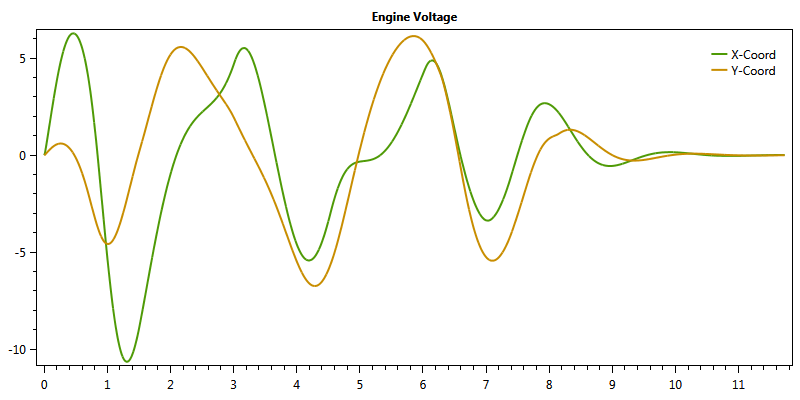
\includegraphics[width = 350pt]{WindPDEV} 
		\caption{\textit{Wpływ siły wiatru na układ sterowany zmodyfikowanym podwójnym regulatorem równoległym: wykres zależności napięcia na silniku od czasu}}
		\label{plot:WindPDEV}
\end{figure}

\begin{figure}[H]
	\centering
		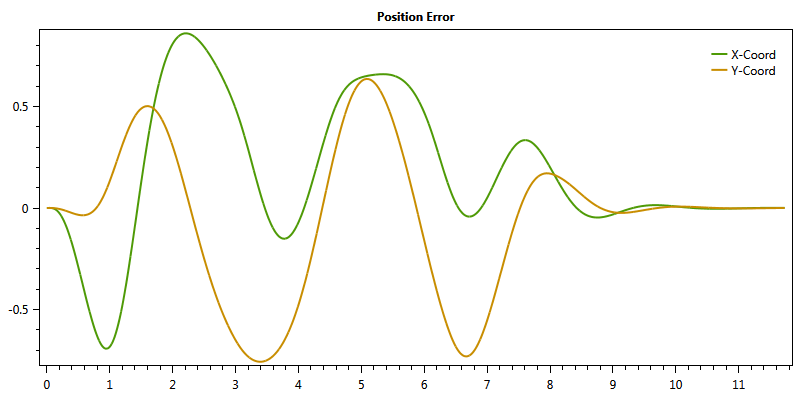
\includegraphics[width = 350pt]{WindPDCEP} 
		\caption{\textit{Wpływ siły wiatru na układ sterowany zmodyfikowanym podwójnym regulatorem równoległym: wykres zależności uchybu pozycji od czasu}}
		\label{plot:WindPDCEP}
\end{figure}

\begin{figure}[H]
	\centering
		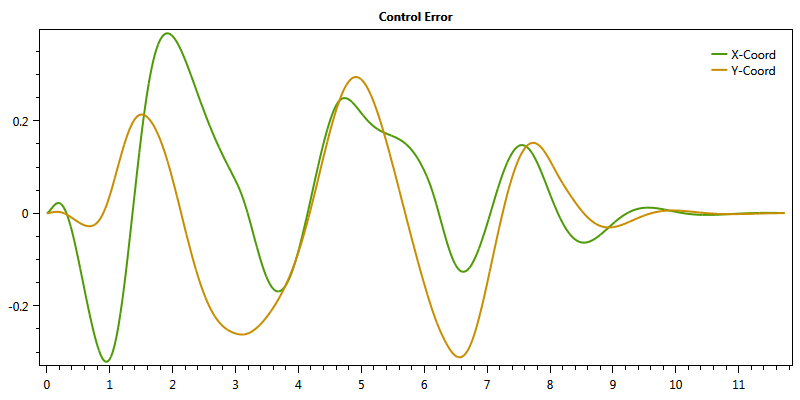
\includegraphics[width = 350pt]{WindPDCEA} 
		\caption{\textit{Wpływ siły wiatru na układ sterowany zmodyfikowanym podwójnym regulatorem równoległym: wykres zależności uchybu kąta od czasu}}
		\label{plot:WindPDCEA}
\end{figure}

W przypadku regulatora podwójnego konieczność utrzymania stałej pozycji powoduje znaczne wychylenia wahadła. Wraz ze wzrostem mocy wiatru układ wymaga coraz większej ingerencji ze strony kontrolera. W celu przeciwstawienia się zakłóceniu regulator nakazuje układowi utrzymywanie wychylenia w kierunku przeciwnym do kierunku siły wiatru. Usunięcie zakłócenia pozwala układowi na powrót do stabilnej pozycji początkowej. 

Dla symulacji z prostym regulatorem PID sytuacja wygląda zupełnie inaczej. Układ nie potrzebuje utrzymania stałej pozycji, wobec czego poddaje się sile wiatru poruszając się w zadanym przez nią kierunku. Regulator pozwala na utrzymanie bezpiecznego wychylenia niezależnie od mocy zakłócenia. Po zakończeniu oddziaływania zewnętrznego układ nie wraca do punktu startowego, stabilizowane jest jedynie odchylenie wahadła od osi pionowej.


%% -------- chapter V --------
\chapter{Architektura systemu}
\section{Ogólny opis rozwiązania}
Opracowany symulator jest aplikacją okienkową przeznaczoną na komputery z systemem Windows, wykonaną w technologii .NET 4.5 za pomocą pakietu Microsoft Visual Studio 2015. Program zbudowany został na bazie platformy Windows Presentation Foundation, z wykorzystaniem bibliotek HelixToolkit, OxyPlot oraz narzędzi do obliczeń numerycznych i symbolicznych (szczegóły omówione w sekcji \ref{Tools}). Koncepcja symulacji została podzielona na dwa zasadnicze zagadnienia: uniwersalna biblioteka fizyki oraz graficzna aplikacja wizualizacji. Istotną częścią pracy jest również zagadnienie komunikacji między modułami oraz charakterystyka pracy symulatora.

\subsection{Symulator}
Wiele programów symulacyjnych posiada zaawansowane możliwości techniczne, jednakże bez odpowiedniej oprawy graficznej i interakcji stają się narzędziami mało użytecznymi. Autor pracy dołożył wszelkich starań, by stworzyć rozwiązanie proste, pozwalające na intuicyjne wykorzystywanie wszystkich funkcjonalności. Ponadto za główny cel aplikacji przyjęto maksymalizację możliwości modyfikowania poszczególnych parametrów i wizualizację wszystkich kluczowych cech badanego układu. 

Podział symulatora na elementy składowe przestawiony został na schemacie \ref{SystemVisual}.

\begin{figure}[H]
	\centering
		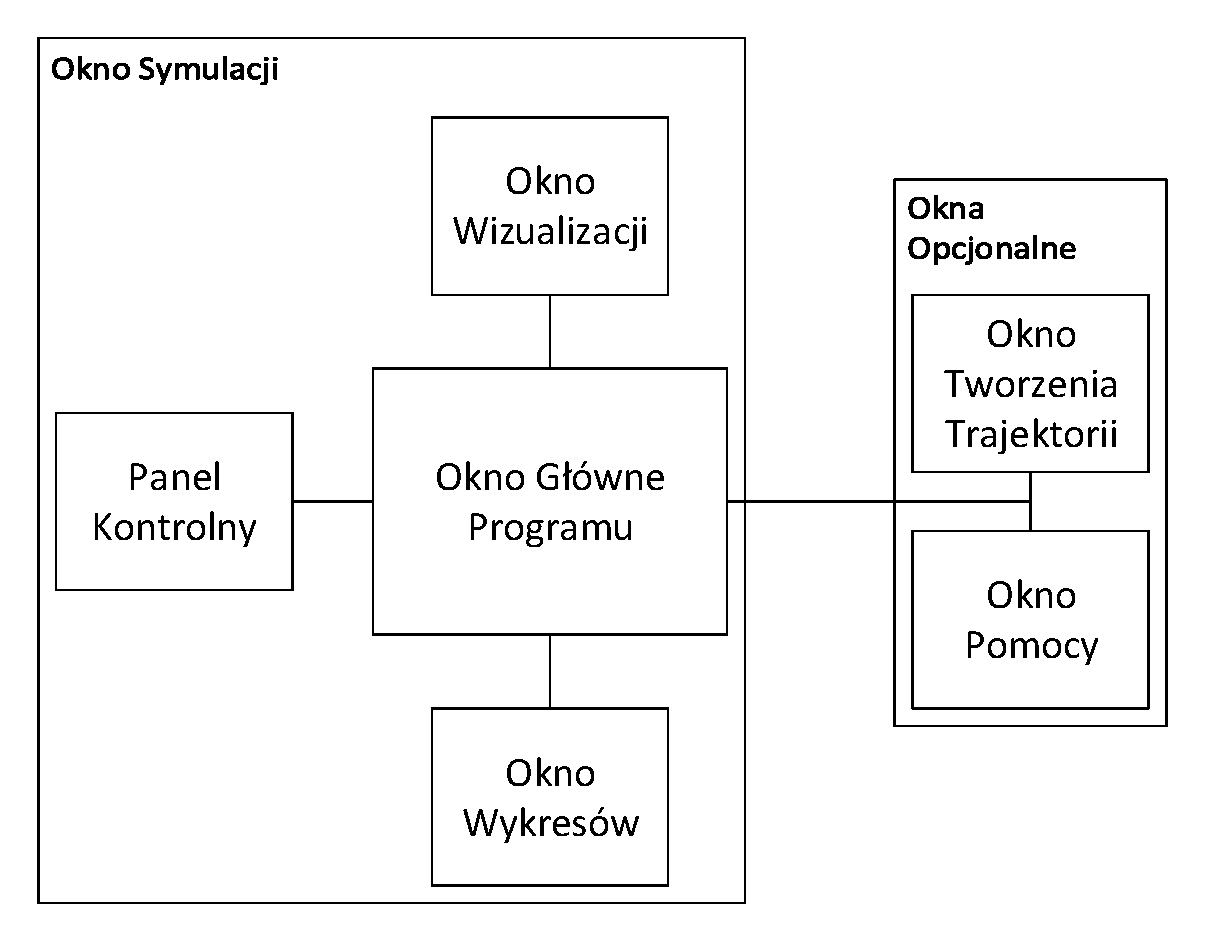
\includegraphics[width = 300pt]{SystemVisual} 
		\caption{\textit{Diagram komponentów wizualnych aplikacji}}
		\label{SystemVisual}
\end{figure}

Główne okno symulacji (\texttt{MainWindow}) składa się z trzech współpracujących ze sobą elementów. Są to:
\begin{itemize}
\item Okno wizualizacji - zarządzane przez moduł \texttt{SceneControl}, odpowiedzialne za tworzenie, modyfikację i aktualizację stanu wizualizacji.
\item Okno wykresów - nadzorowane przez moduł \texttt{PlotsControl}, zajmuje się konfiguracją i wyświetlaniem dynamicznych wykresów dla danych symulacji. 
\item Panel kontrolny - integralna część okna głównego aplikacji, odpowiedzialna za interakcję z użytkownikiem. Moduł obejmuje zarządzanie ustawieniami oraz przekazywanie informacji o modyfikacjach parametrów.
\end{itemize}

Dodatkowymi elementami są okna wyświetlane na żądanie:
\begin{itemize}
\item Okno tworzenia trajektorii - ekran pozwalający zdefiniować parametry nowej trajektorii, otwierany opcjonalnie poprzez element panelu kontrolnego.
\item Okno pomocy - dynamiczny widok interakcyjny prezentujący funkcjonalności poszczególnych elementów symulatora, podobnie jak poprzednie okno, włączane opcjonalnie z panelu kontrolnego.
\end{itemize}

\newpage
Wszystkie elementy graficzne symulatora zostały wykonane przy pomocy dedykowanego dla technologi WPF języka XAML, ze szczególną dbałością o adaptację do różnych rozdzielczości ekranu. Logika systemu została zaimplementowana w języku C\#. Główna pętla symulacji została oparta o narzędzie \texttt{DispatcherTimer}, które pozwala na cykliczne wykonywanie określonych działań. Czas przebiegu symulacji został uzależniony od modyfikowalnego parametru, dzięki czemu użytkownik ma możliwość sterowania tempem animacji. Aplikacja graficzna zajmuje się wyłącznie prezentowaniem rezultatów obliczeń wykonywanych przez bibliotekę fizyki. Fakt ten umożliwia dowolną modyfikację kształtu symulatora bez obaw o utratę stabilności wykonywanych obliczeń. 

\subsection{Biblioteka fizyki}
Jednym z głównych celów, które autor pracy przyjął za obowiązkowe do zrealizowania było stworzenie jednego komponentu gromadzącego wszystkie zagadnienia związane z fizyką układu. Użyta technologia pozwoliła na zbudowanie w pełni funkcjonalnej biblioteki, która może zostać wykorzystana nie tylko przez aplikację symulatora, lecz również dowolny inny projekt wspierający technologię .NET. Założenie to umożliwia rozbudowę projektu o nową aplikację graficzną stworzoną w dowolnym  środowisku, np. Unity. 

Podział komponentów biblioteki pokazany został na schemacie \ref{Library}.
\begin{figure}[H]
	\centering
		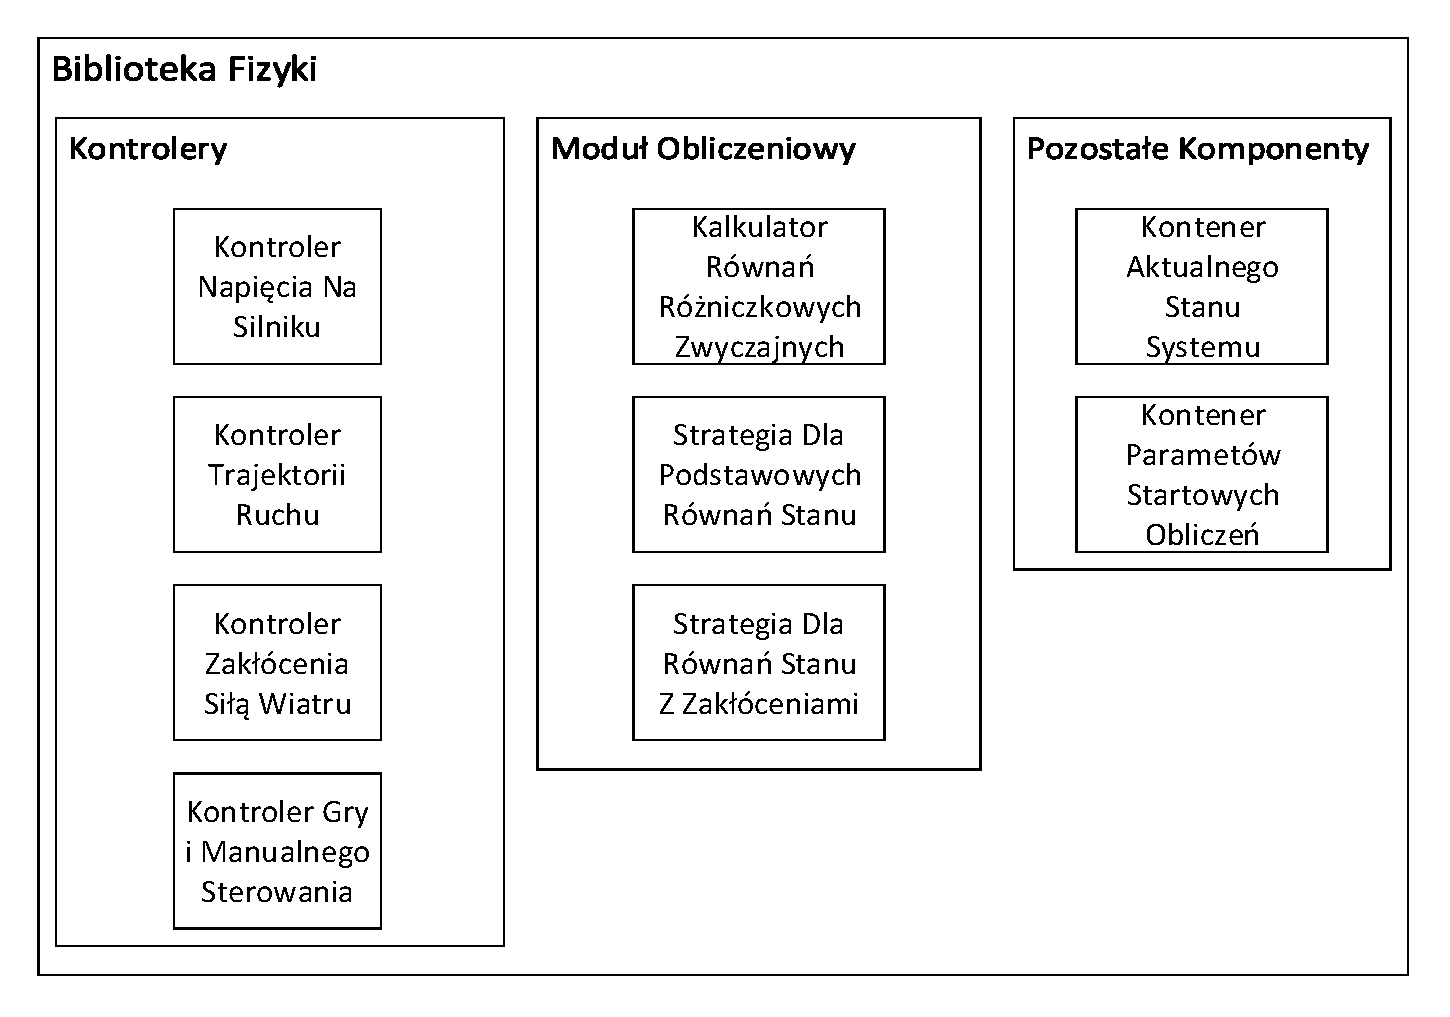
\includegraphics[width = 350pt]{Library} 
		\caption{\textit{Diagram komponentów biblioteki fizyki}}
		\label{Library}
\end{figure}

Biblioteka fizyki obejmuje trzy podstawowe grupy obiektów:
\begin{itemize}
\item Kontrolery - narzędzia sterujące wszystkimi rozszerzeniami podstawowego modelu układu, tj:
\begin{itemize}
\item Kontroler Napięcia Na Silniku (\texttt{VoltageController}) - stabilizator układu. Pozwala na wybór jednego z wielu regulatorów. Gromadzi informacje o uchybie układu oraz wyznacza wynikowe napięcie na silniku.
\item Kontroler Trajektorii Ruchu (\texttt{TrajectoryController}) - umożliwia odczyt i zapis dowolnych trajektorii ruchu. Wyznacza kierunek poruszania dla zadanej pozycji układu.
\item Kontroler Zakłócenia Siłą Wiatru (\texttt{WindController}) - generator losowego zakłócenia identyfikowanego jako siła wiatru. Pozwala na konfigurację typu siły oraz przekazuje aktualny kierunek i moc wiatru.
\item Kontroler Gry i Manualnego Sterowania (\texttt{GameController}) - obsługuje interakcję użytkownika z układem dynamiki. Umożliwia manualne sterowanie wychyleniem układu.
\end{itemize}
\item Moduł Obliczeniowy - zawiera kalkulator rozwiązujący układy równań różniczkowych zwyczajnych metodami Rungego-Kutty. Pozwala na ustalanie różnych strategii obliczeń w zależności od typu układu.
\item Pozostałe Komponenty - elementy wspólne dla całej biblioteki. Są to kontenery danych dotyczących aktualnego stanu całego systemu dynamiki oraz parametrów startowych obliczeń numerycznych. 
\end{itemize}

Każdy z opisanych obiektów udostępnia interfejs podstawowych funkcjonalności. Ponadto przygotowane rozwiązania umożliwiają szeroką gamę rozszerzeń, zarówno w kwestii kontroli, jak i samego kształtu układu dynamiki.

\subsection{Komunikacja}
Podział systemu na moduły wymaga dodatkowego opracowania schematu wzajemnej interakcji między poszczególnymi elementami. Brak jednoznacznie zdefiniowanych reguł przyczyniłby się do ryzyka utraty kontroli nad pracą symulatora, a także możliwością błędnego działania całego systemu. Aby uniknąć przedstawionych problemów stworzony został model komunikacji między najważniejszymi komponentami programu, przedstawiony na diagramie \ref{Interaction}.

\begin{figure}[H]
	\centering
		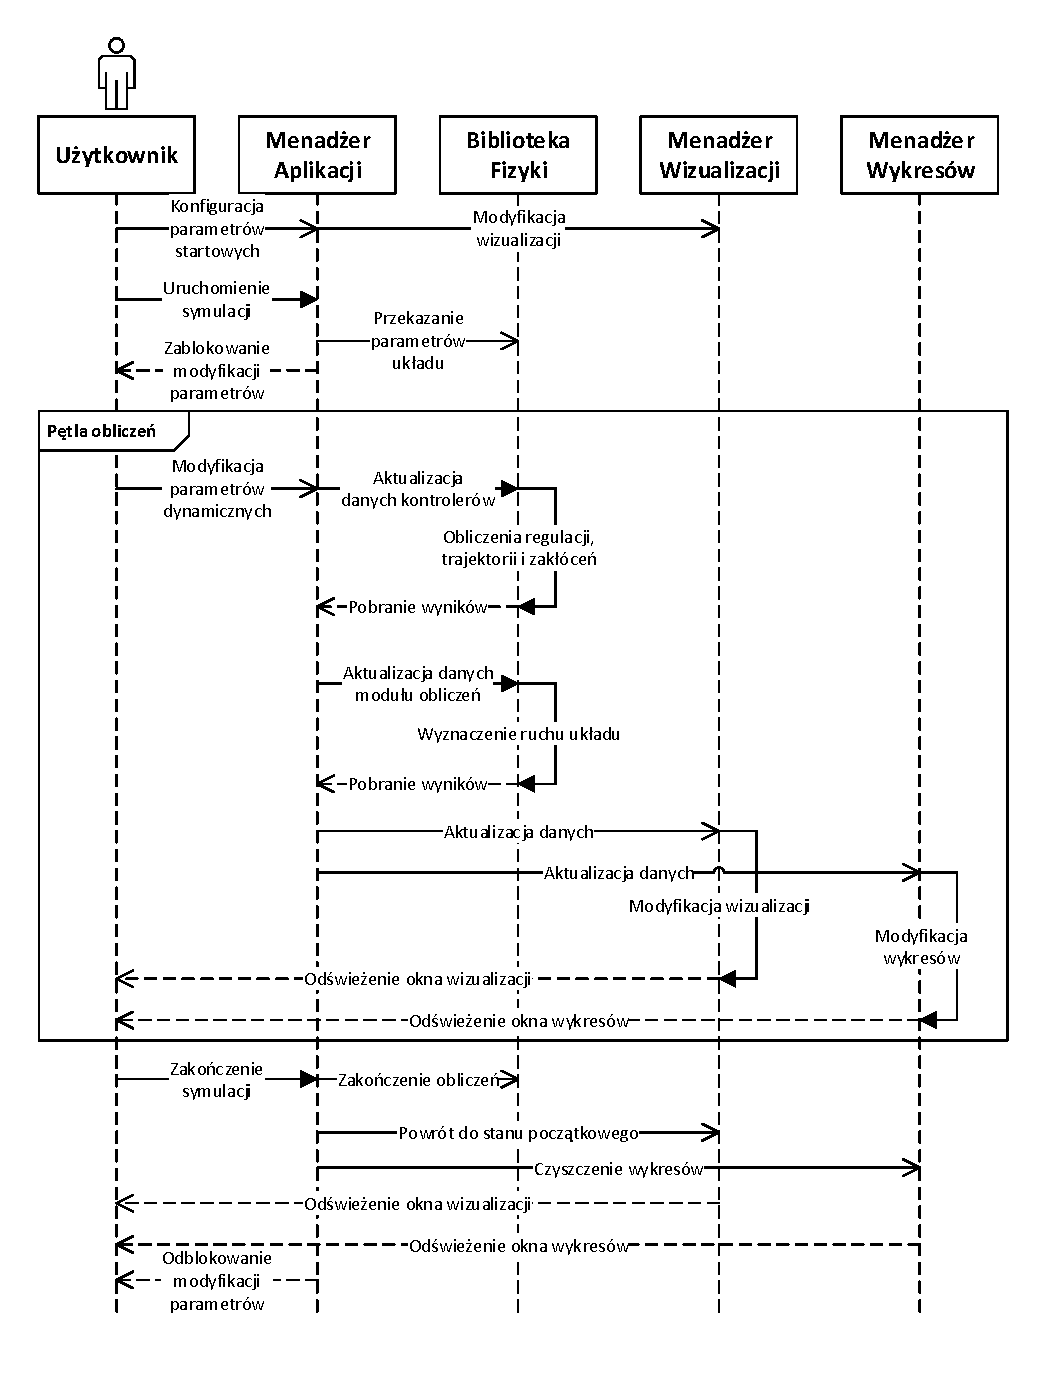
\includegraphics[width = 400pt]{Interaction} 
		\caption{\textit{Diagram interakcji między modułami}}
		\label{Interaction}
\end{figure}

Model zakłada, że system zbudowany jest z czterech podstawowych elementów obejmujących bibliotekę fizyki oraz wizualizację opartą na trzech komponentach reprezentowanych przez menadżerów: aplikacji, wizualizacji i wykresów. Dodatkowo diagram uzupełniony jest poprzez aktora będącego użytkownikiem systemu. 

Komunikacja użytkownika z symulatorem odbywa się wyłącznie poprzez menadżera aplikacji. Użytkownik ma możliwość modyfikacji parametrów systemu i sterowania przebiegiem symulacji. W sytuacji dowolnej zmiany menadżer aplikacji ma obowiązek poinformować o zdarzeniu odpowiednie moduły powiązane z danym parametrem. W przypadku gdy użytkownik przystępuje do rozpoczęcia symulacji, menadżer aplikacji wysyła ustalone parametry układu do biblioteki fizyki, równocześnie blokując użytkownikowi ich modyfikację w trakcie trwania symulacji. Następnie w pętli menadżer aplikacji na bieżąco powiadamia bibliotekę fizyki o aktualnym stanie wszystkich elementów dynamicznych systemu. Biblioteka dokonuje wstępnych obliczeń poprzez narzędzia kontrolerów i przesyła wyniki do głównego menadżera, które trafiają później do modułu obliczeniowego. Biblioteka fizyki wyznacza ruch układu i przekazuje rezultaty do menadżera aplikacji. W kolejnym kroku odpowiednie dane zostają wysyłane do menadżerów wizualizacji i wykresów. Komponenty dokonują aktualizacji danych i modyfikacji stanu odpowiednich elementów. Po wykonaniu wszystkich czynności wyniki pracy prezentowane są użytkownikowi. W przypadku, gdy użytkownik zechce zakończyć symulacje, menadżer aplikacji rozsyła wszystkim pozostałym komponentom informację o zakończeniu obliczeń i konieczności powrotu do stanu początkowego. Wynik akcji prezentowany jest użytkownikowi. Ponadto menadżer aplikacji odblokowuje użytkownikowi możliwość modyfikacji parametrów.

\section{Wykorzystane narzędzia}
\label{Tools}
Niniejsza sekcja poświęcona jest opisowi narzędzi wykorzystanych do realizacji projektu. Autor pracy dołożył starań, by wybrane technologie umożliwiły sprawną implementację systemu, gwarantując uniwersalność i łatwą przenośność rozwiązania. Istotnym  celem było stworzenie biblioteki fizyki, której użycie nie wymagałoby instalacji dodatkowego oprogramowania matematycznego. Głównym wymaganiem wobec wizualizacji było wybranie narzędzi pozwalających na wykonanie rozwiązania prostego w obsłudze, przejrzystego oraz możliwego do uruchomienia przez wielu użytkowników.

\subsubsection{Windows Presentation Foundation}

Windows Presentation Foundation (WPF) jest to platforma służąca do wytwarzania aplikacji przeznaczonych na systemy okienkowe. Technologia wchodzi w skład pakietu oprogramowania .NET Framework dostarczanego przez firmę Microsoft. Narzędzie pozwala na budowanie zaawansowanych programów wykorzystujących interfejs użytkownika, multimedia oraz grafikę trójwymiarową. WPF korzysta z języka XAML, będącego implementacją języka XML. Język ten umożliwia realizację deklaratywnego modelu programowania. Technologia wykorzystuje zaawansowany sprzęt graficzny poprzez odpowiedni silnik wyświetlania, który cechuje się niezależnością od rozdzielczości ekranu oraz wykorzystaniem techniki wektorowej i akceleracji grafiki 3D. Dodatkowe informacje oraz poradniki użytkowania można znaleźć pod adresem \cite{WPF}.

Technologia umożliwia łatwą separację graficznego interfejsu użytkownika od logiki biznesowej poprzez implementację wzorca architektonicznego MVVM. Powala to na definiowanie modelu danych za pomocą kodu w języku C\# oraz wyświetlanie graficznej reprezentacji danych przy użyciu języka znaczników. Niezbędny w tym procesie jest konwerter danych zwany widokiem dla danego modelu. WPF upraszcza wykonanie wzorca poprzez wbudowane narzędzie dowiązań.

Autor pracy chcąc uzyskać separację modelu układu od jego graficznego wyglądu wykorzystał przedstawione wyżej funkcjonalności. Ponadto użycie technologii WPF pozwoliło na stworzenie symulatora prostego w obsłudze, intuicyjnego i wyposażonego w zaawansowany moduł wizualizacji.

\subsubsection{HelixToolkit}
Helix Toolkit to otwarta biblioteka grafiki 3D przeznaczona na platformę Windows Presentation Foundation. Narzędzie pozwala na zaawansowaną pracę z grafiką trójwymiarową, w tym: generowanie i wyświetlanie podstawowych modeli, intuicyjna manipulacja kamerą, dynamiczne wyświetlanie animacji. Dokładny opis technologii wraz z dokumentacją techniczną dostępne są na stronie \cite{HelixToolkit}.

Decyzja o wyborze wspomnianego narzędzia została oparta o doświadczenie w pracy z biblioteką oraz wykorzystanie jej w projekcie obejmującym zbliżoną tematykę.

\subsubsection{OxyPlot}
OxyPlot jest to otwarta biblioteka przeznaczona na platformę .NET służąca do generowania wykresów. Technologia umożliwia dynamiczne tworzenie zaawansowanych wykresów, modyfikację sposobu wyświetlania danych oraz eksport rezultatów do pliku. OxyPlot współpracuje z platformą WPF i umożliwia tworzenie dowiązań danych do konkretnego graficznego okna wykresu. Wszystkie niezbędne informację na temat biblioteki dostępne są pod adresem \cite{OxyPlot}.

Podobnie jak w przypadku poprzedniej technologii wybór rozwiązania podyktowany był dobrą znajomością narzędzia oraz użyciem go w wielu projektach poświęconych symulacji. 


\subsubsection{Pozostałe}
W projekcie wykorzystano dodatkowe narzędzia realizujące pojedyncze funkcjonalności. Część rozwiązań mogłaby być zrealizowana samodzielnie przez autora pracy, jednakże na etapie analizy wstępnej przyjęto, że zadania te nie są głównym celem pracy i do zrealizowania ich należy użyć gotowych narzędzi. Są to:
\begin{itemize}
\item ALGLIB - wieloplatformowa, otwarta biblioteka obliczeń numerycznych. Narzędzie pozwala na analizę danych, optymalizację oraz rozwiązywanie problemów z zakresu algebry liniowej. Autor pracy skorzystał z pakietu obliczeń układów równań różniczkowych metodami Rungego-Kutty z adaptacyjnym krokiem całkowania (algorytm opisany w sekcji \ref{Runge}). 
\item FParsec - otwarta biblioteka przeznaczona na platformę .NET, służąca do analizy tekstów pod kątem konkretnych gramatyk formalnych. Pakiet umożliwia rozpoznawanie matematycznych wyrażeń symbolicznych. Narzędzie to było pomocne przy analizie parametryzacji krzywej w module tworzenia nowych trajektorii.
\item Math.NET Symbolics - otwarta biblioteka obliczeń symbolicznych dedykowana dla platformy .NET. Narzędzie pozwala na rozwiązywanie równań symbolicznych. Autor pracy użył pakietu do wyznaczania punktów kontrolnych krzywych nowo generowanych trajektorii.
\end{itemize}

\section{Wzorce projektowe}
Implementacja systemu realizowana była w zgodzie ze standardami inżynierii oprogramowania. Jednym z kluczowym elementów analizy konstrukcji programu jest zapewnienie łatwej rozszerzalności poszczególnych komponentów. Aby osiągnąć postawiony cel należy dokładnie odseparować poszczególne funkcjonalności oraz zbudować narzędzie zarządzające pracą całej aplikacji. Podział programu na moduły upraszcza kontrolę działania systemu oraz pozwala na dowolne modyfikacje konkretnych elementów bez utraty ogólnej funkcjonalności. Użytecznym rozwiązaniem pomagającym uschematyzować budowę systemu są wzorce projektowe czyli uniwersalne i sprawdzone techniki rozwiązywania określonych problemów projektowych. 

Ze względu na ograniczoną objętość systemu jak również zgromadzenie całej funkcjonalności układu dynamiki w jednej bibliotece, autor pracy nie był zmuszony do rozwiązywania skomplikowanych problemów projektowych wymagających użycia rozbudowanych wzorców. Budowa aplikacji okienkowej realizowana była w zgodzie ze standardami wzorca architektonicznego MVVM. Projekt systemu zakładał łatwy dostęp do wszystkich modeli i ich kontroli, wobec czego nie było potrzeby wprowadzania dodatkowych schematów. W przypadku samej biblioteki fizyki skupiono się na stworzeniu modelu z możliwością modyfikacji dynamiki układu. W celu zapewnienia wymienności definicji i sposobu rozwiązywania równania stanu skorzystano z czynnościowego wzorca projektowego strategii.

Strategia jest to wzorzec definiujący grupę wymiennych algorytmów zebranych w postaci klas. Technika pozwala na łatwą zamianę realizacji problemu w zależności od zaistniałych potrzeb. Diagram opisujący strukturę wzorca przedstawia schemat \ref{StrategyPattern}.

\begin{figure}[H]
	\centering
		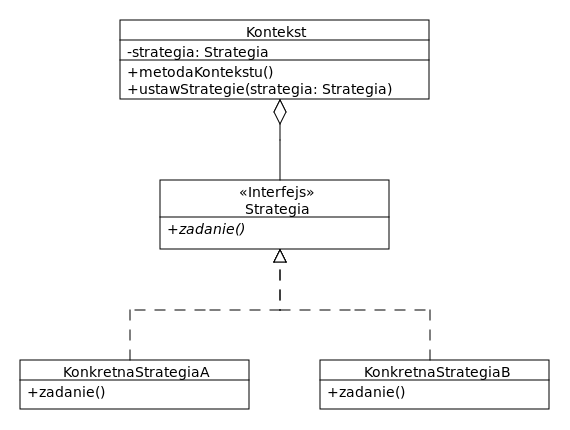
\includegraphics[width = 275pt]{StrategyPattern} 
		\caption{\textit{Diagram klas UML wzorca projektowego Strategia}}
		\label{StrategyPattern}
\end{figure}

Strategia deklaruje interfejs wspólny dla wszystkich sposobów rozwiązania problemu, który gromadzi niezbędne operacje. Każdy z konkretnych algorytmów implementowany jest w postaci klasy realizującej wspomniany interfejs. Dodatkowo definiowany jest klient, którego zadaniem jest wybór i przechowywanie konkretnej strategii. 

Wzorzec pozwala na definiowanie dowolnej grupy algorytmów i swobodną wymianę ich, w zależności od potrzeb. Ponadto technika ta pozwala na ograniczenie ilości instrukcji warunkowych i łatwe porównanie wyników poszczególnych metod. Wadą rozwiązania jest zwiększenie narzutu na komunikację i zwiększenie ilości obiektów w systemie.

W stworzonym projekcie rolę klienta pełni moduł obliczeniowy, który ustala strategię kształtu i sposobu rozwiązywania równań stanu układu. Konkretnymi strategiami są: układ dynamiki w wersji podstawowej oraz zmodyfikowanej o wpływ zakłóceń. 

\section{Komponenty aplikacji}
W celu uporządkowania struktury systemu oraz zapewnienia stabilnego zarządzania komponentami opracowano uniwersalne własności zrealizowane w postaci interfejsów. Rozszerzenie systemu o kolejne elementy osiągalne jest poprzez realizację poszczególnych interfejsów oraz stworzenie konkretnej implementacji funkcjonalności. Podejście to zapewnia dodatkowo kontrolę nad cyklem wykonywania operacji oraz pomaga ustalić w jakich sytuacjach powinny być wywoływane określone metody.

\subsection{Modele}
Hierarchia klas dla modeli pokazana została na diagramie \ref{IModel}.  

\begin{figure}[H]
	\centering
		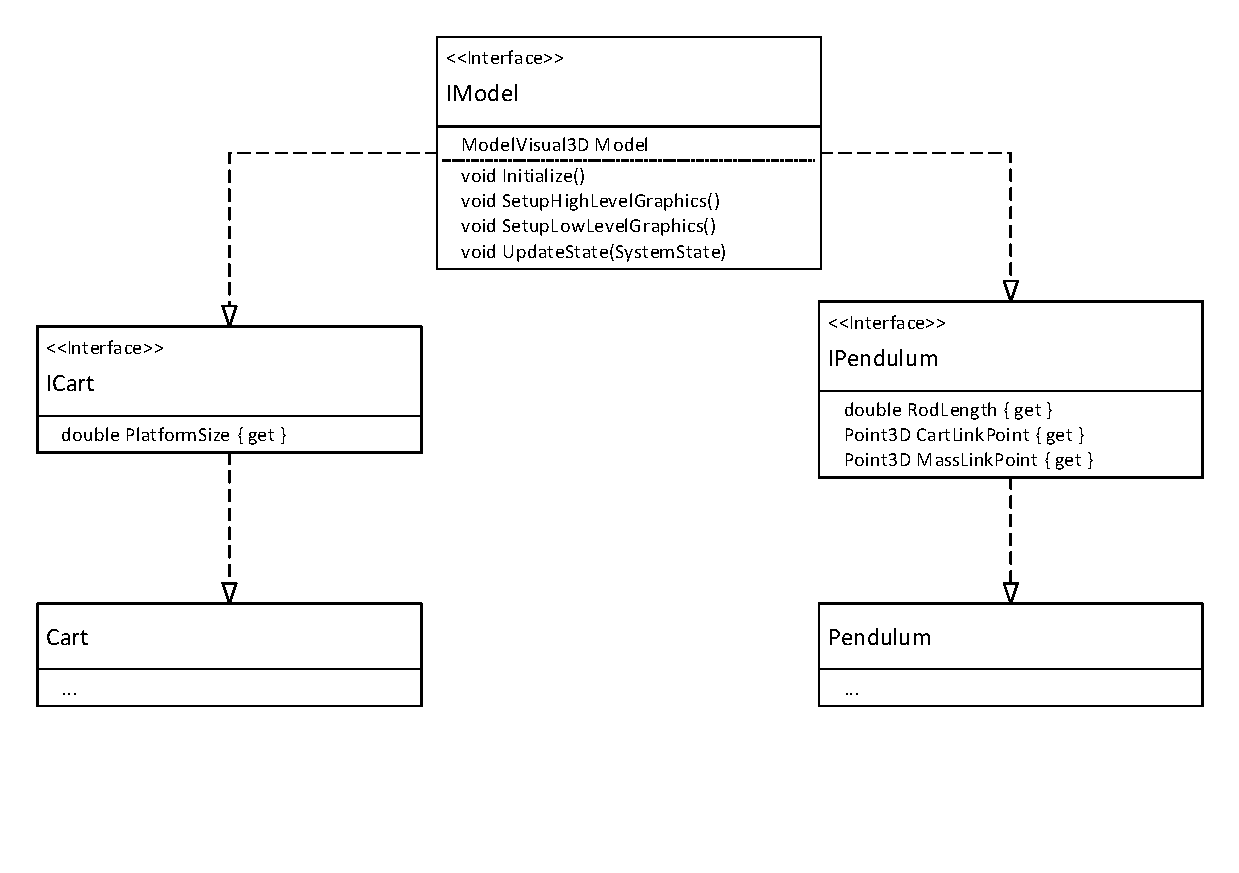
\includegraphics[width = 400pt]{IModel} 
		\caption{\textit{Diagram klas UML dla zarządzania modelami}}
		\label{IModel}
\end{figure}

Wszystkie elementy wizualizacji spełniają wymagania określone poprzez interfejs \texttt{IModel}. Interfejs ten gromadzi podstawowe funkcjonalności niezależne od specyfiki konkretnego modelu, przede wszystkim referencję do całego modelu oraz ustalanie sposobu wyświetlania i aktualizacji. 

Poszczególne obiekty w scenie zaimplementowane zostały jako klasy udostępniające metody poprzez dedykowane interfejsy. Dodatkowo każdy z interfejsów realizuje bazowy interfejs wspólny. 

Zaproponowany schemat pozwala na równoczesną kontrolę nad wszystkimi elementami w scenie oraz daje możliwość łatwego rozszerzania wizualizacji o kolejne elementy.

\subsection{Kontrolery}
Hierarchia klas dla kontrolerów pokazana została na diagramie \ref{IController}.  

\begin{figure}[H]
	\centering
		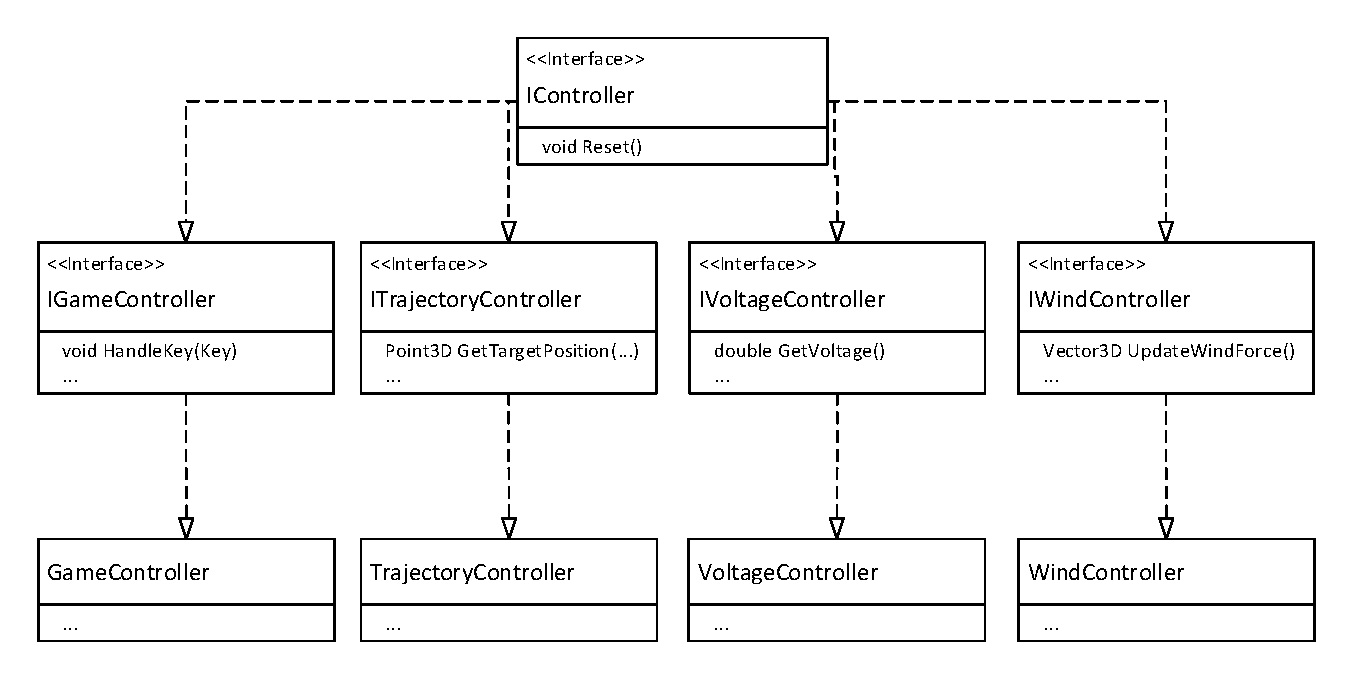
\includegraphics[width = 400pt]{IController} 
		\caption{\textit{Diagram klas UML dla zarządzania kontrolerami}}
		\label{IController}
\end{figure}

Kontrolery są integralną częścią biblioteki fizyki odpowiedzialną za rozszerzanie funkcjonalności układu. Każdy z kontrolerów podlega tym samym regułom budowy. Interfejs \texttt{IController} zbiera wspólne funkcjonalności, natomiast poszczególne dedykowane interfejsy rozszerzają bazę metod do grupy adekwatnej danemu kontrolerowi. 

Przyjęte rozwiązanie, podobnie jak w przypadku modeli, wprowadza porządek i ułatwia zarządzanie wszystkimi narzędziami. Dodatkowo struktura jednoznacznie definiuje w jaki sposób należy dodawać kolejne kontrolery.

%% -------- chapter VI --------
\chapter{Instrukcja użytkownika}
\section{Ogólny wygląd aplikacji}
Symulator został wykonany jako aplikacja okienkowa na urządzenia z systemem Windows. Warunkiem uruchomienia programu jest posiadanie platformy .NET w wersji 4.5. 

Okno programu podzielone zostało na trzy sekcje:
\begin{itemize}
\item Panel kontrolny - służący do konfiguracji ustawień programu i modyfikacji parametrów układu.
\item Okno wizualizacji - obejmuje trójwymiarową scenę z umieszczonym w niej modelem układu. Wyświetla zachowanie układu w zadanych warunkach.
\item Panel wykresów i informacja o stanie układu - umożliwia śledzenie aktualnych parametrów układu oraz przyłożonego sterowania.
\end{itemize}

Przykładowe podglądy aplikacji w trakcie wykonywania poszczególnych symulacji zaprezentowano na ilustracjach \ref{Application} i \ref{Simulation}.

\begin{figure}[H]
	\centering
		\includegraphics[width = 400pt]{Application} 
		\caption{\textit{Podgląd aplikacji w trakcie wykonywania symulacji z manualnym sterowaniem}}
		\label{Application}
\end{figure}

\begin{figure}[H]
	\centering
		\includegraphics[width = 400pt]{Simulation} 
		\caption{\textit{Podgląd aplikacji w trakcie wykonywania symulacji śledzenia trajektorii}}
		\label{Simulation}
\end{figure}

Wszystkie najistotniejsze informacje odnośnie systemu, wraz z wygodnym trybem pomocy znajdują się w zakładce \texttt{About} w panelu górnym aplikacji. Dokładny opis poszczególnych funkcjonalności przedstawiony zostanie w kolejnych sekcjach dokumentu.

\section{Konfiguracja}
\subsection{Moduły}
W panelu górnym w zakładce \texttt{Mode} zebrane zostały wszystkie tryby pracy aplikacji:
\begin{itemize}
\item Stabilizacja wychylenia wahadła. Jest to tryb domyślny. Umożliwia podgląd pracy układu w warunkach określonego sterowania z możliwością uwzględnienia zakłóceń. W przypadku wyboru innego trybu i chęci powrotu do domyślnego należy wybrać opcję \texttt{Clear Trajectory} lub \texttt{Clear Game} w zależności od wybranego trybu.
\item Śledzenie trajektorii. Tryb dostępny po wybraniu opcji \texttt{Load Trajectory}. Pozwala na wczytanie dowolnego pliku w formacie \texttt{".trj"} zawierającego kolejne punkty kontrolne docelowej trajektorii. Po uruchomieniu symulacji układ rozpoczyna śledzenie zadanej drogi. Autor pracy przygotował kilka gotowych trajektorii dostępnych w folderze \texttt{Trajectories}. Dodatkowo użytkownik ma możliwość stworzenia nowej trajektorii poprzez wybór opcji \texttt{Create Trajectory}. W nowo otwartym oknie (pokazanym na ilustracji \ref{CreateTrajectory}) pojawia się możliwość podania parametrycznego opisu krzywej (zależnego od parametru \texttt{"t"}), wartości brzegowych oraz ilości punktów kontrolnych. Po wypełnieniu wszystkich pól, kliknięcie przycisku \texttt{Create Trajectory} stworzy nową trajektorię z możliwością zapisania jej na stałe. Nowo utworzona trajektoria zostanie automatycznie wczytana do programu.
\item Sterowanie manualne. Tryb dostępny po wybraniu opcji \texttt{Load Game}. Podobnie jak w przypadku trybu trajektorii na początku należy wybrać plik z gotową trajektorią. Po uruchomieniu symulacji użytkownik zyskuje możliwość ręcznego sterowania układem. Kontrola odbywa się poprzez klikanie odpowiednich przycisków umieszczonych w dolnej części ekranu wizualizacji lub bezpośrednio z klawiatury za pomocą klawiszy wskazanych na poszczególnych przyciskach.
\end{itemize}

\begin{figure}[H]
	\centering
		\includegraphics[width = 175pt]{CreateTrajectory} 
		\caption{\textit{Okno tworzenia nowej trajektorii}}
		\label{CreateTrajectory}
\end{figure}
\subsection{Opcje}
Symulator umożliwia dostosowywanie ustawień do potrzeb użytkownika. Wszystkie najważniejsze opcje zostały zgromadzone w zakładce \texttt{Options} w panelu górnym aplikacji:
\begin{itemize}
\item Kontroler napięcia na silniku. W zależności od wybranego trybu pracy aplikacja umożliwia ustawienie dowolnego regulatora dla układu:
\begin{itemize}
\item Dla trybu śledzenia trajektorii: regulatory podwójne: równoległe i kaskadowy.
\item Dla trybu stabilizacji: regulator PID oraz regulatory niezależne od uchybu: losowy i sinusoidalny.
\item Dla trybu gry: dowolny regulator.
\end{itemize}
\item Generator siły wiatru. Aplikacja umożliwia wybór jednej z metod losowych wytwarzania zakłócenia dla układu: skokowe lub gładkie.
\item Wyświetlanie trajektorii. Użytkownik ma możliwość włączania i wyłączania wyświetlania w wizualizacji poszczególnych trajektorii: ruchu wózka, ruchu wahadła oraz docelowej trajektorii z pliku.
\item Dokładność śledzenia trajektorii. W zależności od potrzeb algorytm poruszania wzdłuż zadanej drogi będzie pracował z wybraną dokładnością: \texttt{Ultra}, \texttt{High}, \texttt{Medium} lub \texttt{Low}. Domyślną wartością jest: \texttt{Medium}.
\item Jakość wizualizacji. W trakcie trwania symulacji można przełączać tryb wyświetlania między: \texttt{Solid Colors} (dedykowany do obserwacji zachowania układu) a \texttt{Textures} (bardziej atrakcyjny wizualnie, do prezentacji symulatora).
\end{itemize}

\subsection{Sterowanie parametrami}
Symulacja wyróżnia dwa typy parametrów systemu:
\begin{itemize}
\item Parametry startowe. Są to wartości określające stan początkowy układu, takie jak: masy i długości komponentów, początkowe wychylenia oraz krok czasowy animacji. Aplikacja umożliwia sterowanie wartościami parametrów poprzez odpowiednie suwaki. Aktualna wartość wyświetlana jest obok poszczególnego parametru. Po rozpoczęciu symulacji zmiana parametrów jest zablokowana, aż do czasu jej zakończenia. W każdej chwili można przywrócić parametry domyślne poprzez przycisk \texttt{Reset} umieszczony obok zakładki \texttt{System Parameters}.
\item Parametry dynamiczne. Wartości odpowiedzialne za kontrolę zakłóceniami dla układu. Użytkownik ma możliwość zmiany parametrów w trakcie trwania symulacji, w szczególności pojawia się opcja włączenia i wyłączenia siły wiatru poprzez przesunięcie suwaka \texttt{Wind Power} z pozycji 0 na inną wybraną dowolnie. Włączenie zakłócenia sygnalizowane jest pojawieniem się na ekranie wizualizacji strzałki oznaczającej aktualny kierunek wiatru. Dodatkowo regulacja suwaka \texttt{Wind Change Speed} wpływa na szybkość zmiany kierunku, z którego wieje wiatr.
\end{itemize}

\section{Wizualizacja}
\subsection{Kontrola animacji}
Kontrola przebiegu symulacji odbywa się poprzez specjalnie przygotowany panel zarządzania animacją. Panel ten znajduje się w górnej lewej części okna programu. Użytkownik może kontrolować postęp wizualizacji poprzez trzy przyciski:
\begin{itemize}
\item Przycisk \texttt{Play}. Pozwala na uruchomienie symulacji i wznowienie jej po zatrzymaniu.
\item Przycisk \texttt{Pause}. Umożliwia zatrzymanie animacji w dowolnym momencie.
\item Przycisk \texttt{Reset}. Przywraca symulację do stanu początkowego, czyści wykresy i stan układu.
\end{itemize}
\subsection{Scena}
Okno sceny odpowiedzialne jest za prezentację wizualną zachowania układu dynamicznego. Transporter został zbudowany z platformy posiadającej cztery koła (w postaci kul) oraz odwróconego wahadła zaczepionego w środku platformy. Obszar symulacji został ograniczony do odpowiednio dużej powierzchni. W przypadku osiągnięcia brzegu przez układ, transporter zatrzymuje się na krawędzi, aby nie spaść z zadanego podłoża. W celu ułatwienia oceny ruchu układu podłoże zostało pokryte gęstą siatką.

Dodatkowymi elementami na ekranie symulacji są osie układu współrzędnych znajdujące się w lewym dolnym rogu okna, kostka rotacji umieszczona w prawym dolnym rogu oraz licznik klatek na sekundę w górnym prawym rogu.

Użytkownik może dowolnie manipulować umieszczoną w symulacji kamerą. Podstawowe funkcjonalności obejmują:
\begin{itemize}
\item \texttt{Prawy przycisk myszy + przesunięcie} - obrót kamery wokół transportera.
\item \texttt{Środkowy przycisk myszy + przesunięcie} - zmiana kierunku widoku kamery (w czasie przebiegu animacji cel kamery zablokowany jest na pozycji transportera).
\item \texttt{Obrót rolką myszy} - przybliżenie lub oddalenie widoku.
\item \texttt{Kliknięcie kostki rotacji} - obrót kamery do osi głównych związanych z wybraną ścianą kostki.
\end{itemize}

\subsection{Wykresy}
W trakcie trwania symulacji niektóre istotne dane związane z mechanizmem sterowania prezentowane są w formie wykresów. Równocześnie na dwóch wykresach wyrysowywane są informacje na temat napięcia na silniku oraz uchybu kąta dla dwóch podukładów sterujących modelem. Użytkownik w każdej chwili ma możliwość zapisania aktualnie wygenerowanego wykresu poprzez kliknięcie prawym przyciskiem myszy obok tytułu wykresu. Dodatkowo pojawia się możliwość zapisania charakterystyki uchybu pozycji, szczególnie przydatnej przy ocenie jakości ruchu układu do zadanego punktu docelowego.

%% -------- chapter VII --------
\newpage
\chapter{Podsumowanie pracy}
\section{Ocena rozwiązania}
Niniejszy rozdział stanowi podsumowanie całości pracy włożonej w przygotowanie omawianego rozwiązania. Głównym celem projektu było stworzenie symulacji pewnego modelu fizycznego wraz z narzędziem umożliwiającym jego stabilizację i swobodę ruchu. Realizowanie zadania było doskonałą okazją do zapoznania się z metodyką tworzenia oprogramowania symulacyjnego, jak również pozwalało na pogłębienie wiedzy z zakresu rzeczywistości wirtualnej, modelowania układów dynamicznych oraz teorii sterowania. Autor pracy uważa, że czas poświęcony na wykonanie projektu był dobrą inwestycją w rozwój wiedzy i doświadczenia. Istotnym atutem pracy była zbieżność tematyki z zainteresowaniami autora pracy, dzięki czemu ukończenie jej przyniosło dużą satysfakcję. 

Podsumowanie jakościowe pracy rozpatrzono pod kątem stopnia realizacji oraz poprawności wykonania. Każde z kryteriów zostało omówione w poszczególnych sekcjach.

\subsection{Stopień realizacji projektu}
Symulacja spełnia wszystkie kluczowe wygania wypracowane w trakcie analizy wstępnej. Użytkownik końcowy otrzymuje oprogramowanie umożliwiające wnikliwy podgląd pracy układu, wraz z możliwością dowolnego konfigurowania parametrów. Przygotowane narzędzia dają możliwość wprowadzenia różnych trajektorii ruchu, które układ będzie w stanie odwzorować. Dodatkowym atutem jest możliwość nawiązania bezpośredniej interakcji z modelem poprzez moduł ręcznego sterowania. Program pozwala również na badanie zachowania układu w obecności zewnętrznego zakłócenia. Całość pracy, wraz z bazą matematyczno-fizyczną, opisem rozwiązań i testów oraz kwestiami programistycznymi została zebrana w niniejszym dokumencie.

\subsection{Poprawność rozwiązania}
W celu weryfikacji poprawności rozwiązania przeprowadzono gruntowne testy obejmujące zarówno zachowanie układu, jak i pracę całego narzędzia symulacyjnego. W obydwu przypadkach rezultaty były pozytywne, jednoznacznie wskazujące na poprawne zrealizowanie przyjętych zadań.

Opracowane narzędzia pozwoliły dodatkowo na przeprowadzenie dokładnych testów rozpatrywanych koncepcji stabilizacji układu. Wyniki badań jednoznacznie wskazały poziomy użyteczności poszczególnych pomysłów i pozwoliły na wybór najlepszych.

Istotnym sukcesem projektu jest spełnienie przyjętych wymagań niefikcjonalnych. Aplikacja została przetestowana przez grupę użytkowników końcowych. Opinie na temat programu podkreślały jego stabilność, łatwość w obsłudze i interesującą formę prezentacji danych.

\section{Krytyczna refleksja}
W poniższej sekcji autor pracy pragnie podzielić się spostrzeżeniami na temat ewentualnych zmian koncepcji realizacji projektu w sytuacji, gdyby praca miała zostać wykonana ponownie. Charakterystyka ta pozwoli na określenie jak bardzo zdobyta w trakcie wykonywania projektu wiedza przyczyniłaby się do poprawy finalnego kształtu pracy. 

Analiza wstępna projektu skupiła się głównie na pełnej analizie modułu fizyki układu i sterowaniu nim. Pozwoliło to na wypracowanie kompletnej biblioteki fizyki, która może być użyta w dowolnym projekcie. Niestety, w przypadku aplikacji symulatora, dopiero w trakcie realizacji programu autor pracy zdał sobie sprawę, iż narzędzie to powinno być uniwersalnym środowiskiem, umożliwiającym prezentacje zachowania dowolnego modelu dynamiki. W dalszej części projektu postarano się o wypracowanie możliwie uniwersalnego rozwiązania, jednakże dużo łatwiej byłoby osiągnąć pełen efekt, gdyby koncepcja została rozpatrzona na początku prac. 

Kolejną kwestią jest jakość stabilizacji układu dla problemu śledzenia trajektorii. W początkowej fazie projektu autor pracy nie dysponował wystarczającą wiedzą pozwalającą na trafny dobór rozwiązań. Gdyby była możliwość ponownego stworzenia projektu, w pierwszej kolejności dokonano by porównania różnych technik regulacji układu za pomocą narzędzi oferowanych przez pakiety symulacyjne. Prawdopodobnie przyczyniłoby się to do wyboru dodatkowych kontrolerów, m.in. regulatora LQR. Ponadto zwrócono by większą uwagę na optymalizację parametrów użytych metod. Modyfikacja obejmowałaby również samą ideę algorytmu realizowania trajektorii przez układ. Testy wykazały, że niektóre rozwiązania wymagają nieco innego podejścia, by móc uzyskać zmaksymalizowany efekt. 

Ostatnia sprawa dotyczy jakości zrealizowanej wizualizacji. Autor pracy uznał, że nadmiar efektów graficznych przyczyni się do zakrycia istoty realizowanego problemu. Jednakże w trakcie implementacji programu pojawiła się koncepcja podwójnego trybu wyświetlania. Jeden z nich pozwalałby na wnikliwą obserwację dynamiki układu. Drugi natomiast prezentowałby symulację w sposób atrakcyjny dla oka użytkownika końcowego. Brak rozpatrzenia drugiego pomysłu na etapie analizy projektu spowodował, że funkcjonalność ta została zrealizowana jedynie w niewielkim stopniu.

\section{Możliwości rozszerzania projektu}
Zrealizowany projekt obejmuje kilka zagadnień z zakresu modelowania dynamiki, sterowania układem oraz tworzenia symulacji. Dodatkowo zawiera niestandardową koncepcję łączenia prostych dwuwymiarowych układów w jeden duży trójwymiarowy model. Mnogość poruszanych tematów pozwala na szeroką gamę rozszerzeń w zakresie zarówno matematyczno-fizycznym, jak i programistycznym.

Najciekawsze pomysły na wzbogacenie symulatora opracowane przez autora pracy przedstawiono poniżej:
\begin{itemize}
\item Modyfikacja modelu układu - wprowadzenie możliwości definiowania dowolnego obiektu trójwymiarowego, który zastąpiłby model wahadła. Zabieg ten pozwoliłby na zbadanie jakości sterowania dla nietrywialnego modelu. Istotnym zagadnieniem związanym z przedstawionym pomysłem jest konieczność wyznaczania tensora bezwładności dla wybranej bryły. Autor pracy sugeruje wykorzystanie szeroko stosowanej metody Monte-Carlo.
\item Analiza większej ilości regulatorów - autor pracy skupił się na różnych odmianach regulatora PID. Literatura wskazuje na użyteczność innych narzędzi, szczególnie optymalnego regulatora LQR. Porównanie skuteczności wspomnianych kontrolerów dostarczyłoby cennej wiedzy z zakresu teorii sterowania.
\item Rozbudowa modułu zakłóceń - obecna wersja modułu obejmuje gładkie ruchy wiatru w losowych kierunkach. Model ten można zastąpić przez inny bardziej wierny rzeczywistemu. Warto również zwrócić uwagę na zagadnienie prądów powietrznych, których wpływ na układ byłby okazją do zbadania jakości stabilizacji. Ponadto moduł można wzbogacić o inne rodzaje zakłóceń, np. wywołane oddziaływaniami magnetycznymi.
\item Wprowadzanie powierzchni ruchu - symulator prezentuje ruch układu po płaszczyźnie. Interesującym zadaniem byłoby stworzenie nieregularnej powierzchni, z którą układ musiałby się zmierzyć w trakcie wykonywania zadanej trajektorii.
\item Wzbogacenie wizualizacji - rozszerzenie wizualizacji w trybie teksturowym o dodatkowe efekty graficzne. Pomysł nie wnosi istotnego pożytku dla analizy zachowania układu, natomiast stanowi atrakcyjny dodatek dla użytkownika.
\end{itemize} 

Przytoczone koncepcje znajdują uzasadnienie w technice i inżynierii oprogramowania. Jeśli temat miałby być kontynuowany prawdopodobnie wymienione pomysły zostałyby wprowadzone do systemu.
	
%% -------- bibliography --------
\pagestyle{plain}
\begin{thebibliography}{11}

\bibitem{BipedWalking} 
Kajita S., 
\emph{The 3D Linear Inverted Pendulum Mode: A simple modeling for a biped walking pattern generation}, 
2001.

\bibitem{MarciniakControlSystems} 
Marciniak K., 
\emph{Control systems}, 
w: \emph{Modelling in state space}, 
Warszawa, 2003.

\bibitem{MarciniakClosedLoop} 
Marciniak K., 
\emph{Design of closed loop control}, 
w: \emph{Modelling in state space}, 
Warszawa, 2003.

\bibitem{MarciniakDynamicSystems} 
Marciniak K., 
\emph{Dynamic systems}, 
w: \emph{Modelling in state space}, 
Warszawa, 2003.

\bibitem{RungeKutta} 
Neumann E., 
\emph{Runge-Kutta Algorithm}, 
2016,
\\*
http://www.myphysicslab.com/explain/runge-kutta-en.html.

\bibitem{OptimalControl} 
Prasad L., 
\emph{Optimal Control of Non linear Inverted Pendulum Dynamical System with Disturbance Input using PID Controller \& LQR}, 
IEEE, 2011,
\\*
http://ieeexplore.ieee.org/document/6190585/.

\bibitem{LMIP} 
Robles R., Shardt Y., 
\emph{Linear motion inverted pendulum, derivation of the state-space model},
\\*
http://www.jtjt.pl/www/pages/odwrocone-wahadlo/LMIP.pdf.

\bibitem{JTJT} Tyma J., 
\emph{Odwrócone wahadło},
2016,
\\*
http://www.jtjt.pl/odwrocone-wahadlo.

\bibitem{HelixToolkit} 
\emph{Helix Toolkit Documentation}, 
2015,
\\*
http://docs.helix-toolkit.org/.

\bibitem{OxyPlot} 
\emph{OxyPlot Documentation}, 
2016,
\\*
http://docs.oxyplot.org/.

\bibitem{PWNSymulacja} 
\emph{Słownik Języka Polskiego}, 
PWN, 2016,
\\*
http://sjp.pwn.pl.

\bibitem{WPF} 
\emph{Windows Presentation Foundation Documentation}, 
Microsoft, 2016,
\\*
https://msdn.microsoft.com/en-us/library/ms754130(v=vs.110).aspx.

\bibitem{Strategy}  
\emph{Diagram klas UML wzorca projektowego Strategia},
2011,
\\*
https://pl.wikipedia.org/wiki/Plik:Strategy\_classes\_pl.svg.

\bibitem{3DimModel}  
\emph{Gait Pattern Generation: 3D-LIP Model},
2013,
\\*
http://www.wrighteagle.org/en/research/projgait.php.

\bibitem{PID} 
\emph{Schemat blokowy idealnego regulatora PID}, 
2010,
\\*
https://pl.wikipedia.org/wiki/Plik:Schemat\_blokowy\_regulatora\_pid\_ideal-\\nego.svg.

\bibitem{StateSpace} \emph{State space model integral}, 2011,
\\*
https://pl.wikipedia.org/wiki/Plik:State\_space\_model\_integral.png.

\bibitem{EngineeringSimulation} 
\emph{The Importance of Material Properties in Analysis with SolidWorks Simulation}, 
2012,
\\*
http://blogs.solidworks.com/solidworksblog/2012/05/material-properties-in-an-\\alysis.html.

\bibitem{MeteorologySimulation}
\emph{Two tropical Atlantic hurricanes in a high-resolution atmospheric simulation with the HadGEM3 global climate model at a resolution of N512}, 
2012,
\\*
http://www.nature.com/nclimate/journal/v2/n8/fig\_tab/nclimate1639\_F1.htm.

\bibitem{SystemModel} \emph{Wireless Inverted Pendulum Cart},
\\*
http://www.mne.k-state.edu/static/nlc/tiki-index.php?page=S\_H\_Wireless-\\InvertedPendulumCart.

\end{thebibliography}

\appendix
\begin{appendices}
  \chapter{Wykresy parametrów sterowania dla ruchu po złożonej trajektorii}
\label{appenix:A}
  
\section{Podwójny regulator kaskadowy}
\begin{figure}[H]
	\centering
		\includegraphics[width = 400pt]{TrefoilKnotCascadeEV} 
		\caption{\textit{Śledzenie trajektorii węzła koniczynowego poprzez podwójny regulator kaskadowy: wykres zależności napięcia na silniku od czasu}}
		\label{plot:TrefoilKnotCascadeEV}
\end{figure}

\begin{figure}[H]
	\centering
		\includegraphics[width = 400pt]{TrefoilKnotCascadeCE} 
		\caption{\textit{Śledzenie trajektorii węzła koniczynowego poprzez podwójny regulator kaskadowy: wykres zależności uchybu kąta od czasu}}
		\label{plot:TrefoilKnotCascadeCE}
\end{figure}

\section{Podwójny regulator równoległy}
\begin{figure}[H]
	\centering
		\includegraphics[width = 400pt]{TrefoilKnotParallelEV} 
		\caption{\textit{Śledzenie trajektorii węzła koniczynowego poprzez podwójny regulator równoległy: wykres zależności napięcia na silniku od czasu}}
		\label{plot:TrefoilKnotParallelEV}
\end{figure}

\begin{figure}[H]
	\centering
		\includegraphics[width = 400pt]{TrefoilKnotParallelCE} 
		\caption{\textit{Śledzenie trajektorii węzła koniczynowego poprzez podwójny regulator równoległy: wykres zależności uchybu kąta od czasu}}
		\label{plot:TrefoilKnotParallelCE}
\end{figure}

\section{Zmodyfikowany podwójny regulator równoległy}
\begin{figure}[H]
	\centering
		\includegraphics[width = 400pt]{TrefoilKnotPDEV} 
		\caption{\textit{Śledzenie trajektorii węzła koniczynowego poprzez zmodyfikowany podwójny regulator równoległy: wykres zależności napięcia na silniku od czasu}}
		\label{plot:TrefoilKnotPDEV}
\end{figure}

\begin{figure}[H]
	\centering
		\includegraphics[width = 400pt]{TrefoilKnotPDCE} 
		\caption{\textit{Śledzenie trajektorii węzła koniczynowego poprzez zmodyfikowany podwójny regulator równoległy: wykres zależności uchybu kąta od czasu}}
		\label{plot:TrefoilKnotPDCE}
\end{figure}

  \chapter{Wykresy parametrów sterowania dla układu z zakłóceniami}
\label{appendix:B}
\begin{figure}[H]
	\centering
		\includegraphics[width = 400pt]{WindPIDEV} 
		\caption{\textit{Wpływ siły wiatru na układ sterowany regulatorem PID: wykres zależności napięcia na silniku od czasu}}
		\label{plot:WindPIDEV}
\end{figure}

\begin{figure}[H]
	\centering
		\includegraphics[width = 400pt]{WindPIDCEP} 
		\caption{\textit{Wpływ siły wiatru na układ sterowany regulatorem PID: wykres zależności uchybu pozycji od czasu}}
		\label{plot:WindPIDCEP}
\end{figure}

\begin{figure}[H]
	\centering
		\includegraphics[width = 400pt]{WindPIDCEA} 
		\caption{\textit{Wpływ siły wiatru na układ sterowany regulatorem PID: wykres zależności uchybu kąta od czasu}}
		\label{plot:WindPIDCEA}
\end{figure}

  
\end{appendices}


%% -------- statement --------
\selectlanguage{polish}
\clearpage
\pagestyle{empty}
\noindent Warszawa, dnia \today
\vspace{5cm}
\begin{center}
	\LARGE{Oświadczenie}
\end{center}
Oświadczam, że pracę magisterską pod tytułem: ,,Opracowanie symulatora transportera wahadła odwróconego na wózku'', której promotorem jest prof. dr hab. Krzysztof Marciniak, wykonałem samodzielnie, co poświadczam własnoręcznym podpisem.
\vspace{2cm}
\begin{flushright}
...........................................
\end{flushright}

\end{document}

